\documentclass{tufte-book}

\hypersetup{colorlinks}% uncomment this line if you prefer colored hyperlinks (e.g., for onscreen viewing)

% Book metadata
\title{Introduction to Experimental Physics}
\author[Physics 229]{Phys 229}
\publisher{Andrew MacRae}

%%
% If they're installed, use Bergamo and Chantilly from www.fontsite.com.
% They're clones of Bembo and Gill Sans, respectively.
\IfFileExists{bergamo.sty}{\usepackage[osf]{bergamo}}{}% Bembo
\IfFileExists{chantill.sty}{\usepackage{chantill}}{}% Gill Sans

%\usepackage{microtype}

\usepackage{amsmath}

\usepackage{empheq}
% Just some sample text
\usepackage{lipsum}

% Probably don't need thius
\newcommand{\doccls}[1]{\texttt{#1}}% document class name

%%
% For nicely typeset tabular material
\usepackage{booktabs}


% For graphics / images
\usepackage{graphicx}
\setkeys{Gin}{width=\linewidth,totalheight=\textheight,keepaspectratio}
\graphicspath{{Images/}}

% The fancyvrb package lets us customize the formatting of verbatim
% environments.  We use a slightly smaller font.
\usepackage{fancyvrb}
\fvset{fontsize=\normalsize}

%%
% Prints argument within hanging parentheses (i.e., parentheses that take
% up no horizontal space).  Useful in tabular environments.
\newcommand{\hangp}[1]{\makebox[0pt][r]{(}#1\makebox[0pt][l]{)}}

%%
% Prints an asterisk that takes up no horizontal space.
% Useful in tabular environments.
\newcommand{\hangstar}{\makebox[0pt][l]{*}}

%%
% Prints a trailing space in a smart way.
\usepackage{xspace}
% To give mad credit
\newcommand{\TL}{Tufte-\LaTeX\xspace}


% Prints the month name (e.g., January) and the year (e.g., 2008)
\newcommand{\monthyear}{%
  \ifcase\month\or January\or February\or March\or April\or May\or June\or
  July\or August\or September\or October\or November\or
  December\fi\space\number\year
}

% Prints an epigraph and speaker in sans serif, all-caps type.
\newcommand{\openepigraph}[2]{%
  %\sffamily\fontsize{14}{16}\selectfont
  \begin{fullwidth}
  \sffamily\large
  \begin{doublespace}
  \noindent\allcaps{#1}\\% epigraph
  \noindent\allcaps{#2}% author
  \end{doublespace}
  \end{fullwidth}
}

% Custom Colors
\definecolor{greenExample}{RGB}{61,170,61}
\definecolor{greenExampleBack}{RGB}{216,233,213}


\usepackage[many]{tcolorbox}
% Define example environment
\newtcolorbox[auto counter, number within=chapter]{myexample}[2][]
{%
  breakable,
  enhanced,
  colback=white,
  colbacktitle=white,
  arc=0pt,
  leftrule=1pt,
  left skip = 6pt,
  rightrule=0pt,
  toprule=0pt,
  bottomrule=0pt,
  titlerule=0pt,
  colframe=greenExampleBack,
  fonttitle=\normalcolor,
  overlay = 
  {
    \node
    [
      outer sep=0pt,
      anchor=east,
      text width=2.5cm,
      minimum height=4ex,
      fill=greenExampleBack,
      font=\color{greenExample}\sffamily\scshape
    ] 
    at (title.west) {example~\thetcbcounter};
  },
  title=#2,
  #1
}
\newcommand\Solution{\par\textbf{\textsf{Solution}}\par\medskip}

% Generates the index
\usepackage{makeidx}
\makeindex

\begin{document}
% Front matter
\setcounter{chapter}{1}
\frontmatter

% r.1 blank page
%\blankpage

% v.2 epigraphs
\newpage\thispagestyle{empty}
\openepigraph{%
In theory, there is no difference between theory and practice. But, in practice, there is.
}{Yogi Berra%, {\itshape Design, Form, and Chaos}
}
\vfill
\openepigraph{%
A designer knows that he has achieved perfection 
not when there is nothing left to add, 
but when there is nothing left to take away.
}{Antoine de Saint-Exup\'{e}ry}


% r.3 full title page
\maketitle

% r.9 introduction
\cleardoublepage
\chapter*{Introduction}

Wha?
and the use of the \doccls{tufte-book} and \doccls{tufte-handout} document classes.


%%
% Start the main matter (normal chapters)
\mainmatter


\chapter{Fundamental Quantities of Electronics}
\label{ch:fundamentals}

\section{What is Electronics?}

\newthought{Take an electronic device} which can be as simple (a flashlight) or as complicated (a smartphone) as you like. Fundamentally, these devices function by using electric and magnetic fields to push around charged particles which wiggle and bump into one another in just the right way to work as they do. All of this behaviour can be precisely calculated using Maxwell's equations (which you will see very soon in your physics career if you haven't already). Although that is what is truly what is going on ``behind the scenes'', it is a terribly impractical and unpleasant way of thinking about a flashlight. The goal of electronics is to encapsulate all of this complexity into much simpler abstract models. In other words, we want to simplify the flashlight into a cartoon drawing, the flashlight in the same way that we simplify the motor, suspension, and materials of a car in first year physics (figure \ref{fig:abstraction}).

\begin{figure}
  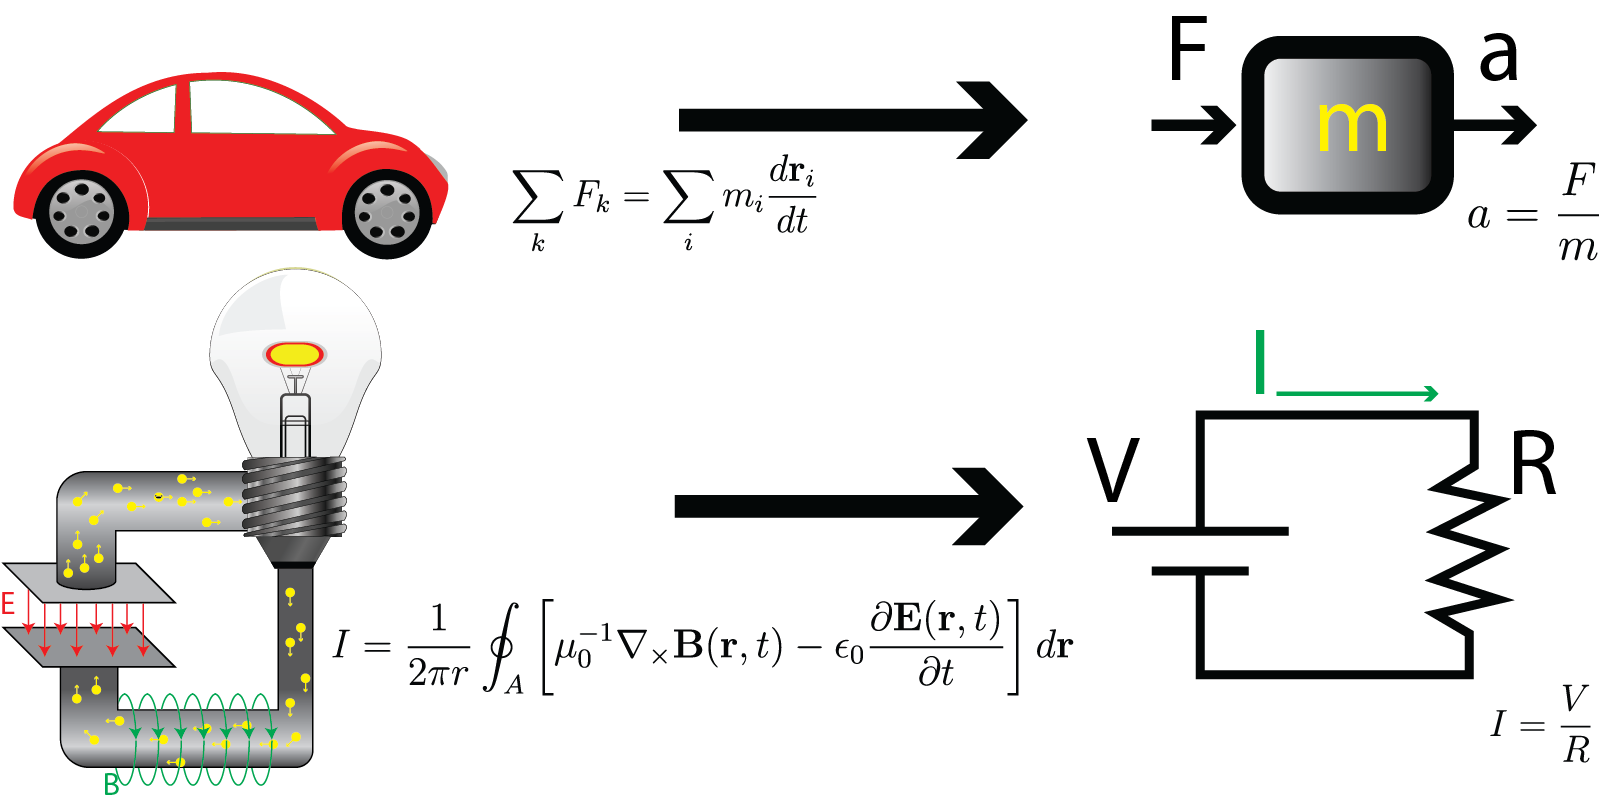
\includegraphics{abstraction}
%  \checkparity This is an \pageparity\ page.%
  \caption{Just as you can calculate the acceleration of a car with mass $m$ and \textit{net} force $F$ without knowing the internal details, the electronics formalism allows you calculate the current through a lightbulb given its resistance and voltage, without bothering about the particular construction or electromagnetic fields.}
  \label{fig:abstraction}
  %\zsavepos{pos:textfig}
  \setfloatalignment{b}
\end{figure}


\section{Fundamental Electronic Quantities: Charge, current, and Voltage}
\subsection{Charge} Charge is a fundamental property of a body and can be negative, positive, or zero (neutral). The S.I. units of charge is the Coulomb [C]. In nature charge is carried by (positive) protons and (negative) electrons\footnote{particle physicists will have a slightly longer list.} having equal magnitude but opposite sign, and the net charge of a body is entirely due to an imbalance between protons and electrons. The charge of an electron is a fundamental constant given approximately by $q_e \approx 1.602\times10^{-19}$ C. 

\subsection{Current} Electronics is concerned with the transport of charge by means of electric and magnetic fields. The force on a charge $q$ due to an electric field $\textbf{E}$ is given by: $\textbf{F} = q\textbf{E}$.\footnote{There is an additional force on a moving charge due to a magnetic field. The more general expression is given by the Lorentz force: $\textbf{F} = q\textbf{E} + q\textbf{v}_\times\textbf{B}$.} The \textit{current} passing through an area $A$ is defined as the amount of charge passing through this area per unit time (see fig. \ref{fig:curr}):

\begin{equation}\label{eq:defn_current_words}
\text{current} = \frac{\text{net charge though surface}}{\text{unit time}}
\end{equation}

\noindent The SI unit of current is the ampere which is a Coulomb per second: 1A = 1C/s.

\begin{marginfigure}%
  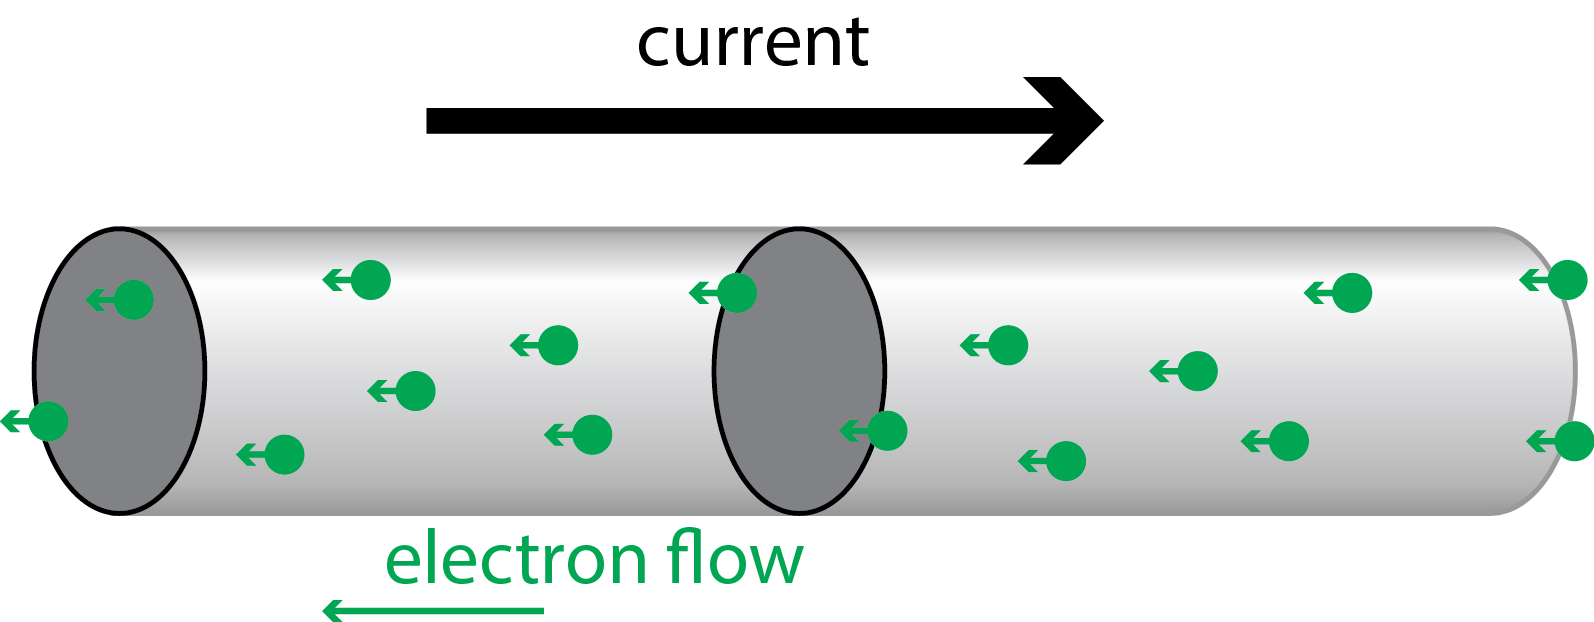
\includegraphics[width=\linewidth]{currentflow}
  \caption{Current in a wire is the amount of charge passing a given cross section of the wire per unit time. Note that due to the negative charge of the electron, the direction of the current is opposite that of the electrons' velocity.}
  \label{fig:curr}
\end{marginfigure}

In electronics we deal with current sufficiently large that we can safely ignore the discrete nature of electrons and treat charge as continuous ``electric fluid'' that can flow (see example \ref{ex:current_is_cts}). This allows us to define the current more rigorously as:
\begin{equation}\label{eq:defn_current}
I \equiv \frac{dq}{dt}
\end{equation}


\begin{myexample}[label = ex:current_is_cts]{The smallest values of current in practice are on the nA ($10^{-9}$A) level. How many electrons pass through a wire per second for 1~nA of Current?}
\Solution
1 nA corresponds to $1\times10^{-9}~\frac{C}{s}$. An electron on the other hand carries approximately $\vert q_e\vert = 1.6\times10^{-19}$~C of charge. A wire conducting 1~nA of current thus sees:
$$
\left(1\times10^{-9}~\frac{C}{s}\right)\times\left(\frac{1~e}{1.6\times10^{-19}C}\right) = 6.25\times10^9\frac{e}{s} 
$$
pass through. Thus, even then, this corresponds to a flow of about 6 billion electrons per second.
\end{myexample}

Note that current is defined to be in the direction of positive charge - the in a typical situation where negatively charged electrons carry the charge, the current is opposite the direction of the charges! 

Typical values for current in electronic devices are on the order of milliamps (1mA = $10^{-3}$A) tens of mA is already dangerous to humans and 1A can easily start fires. We will discuss the heat generated by current shortly. 

\subsection{Voltage/Potential Difference}: You may recall from earlier courses that there is a quantity known as an electric potential $\phi$ which has units  of volts, or equivalently, Newtons per Coulomb (1V = 1N/C). The potential due to a point charge $q$ at distance $r$ is given as $\phi = \frac{1}{4\pi\epsilon_0}\frac{q}{r}$ and the potential due to arbitrary charge distributions can be easily stated\footnote{Though not always easily calculated}. The utility of $\phi$ is that once given it allows you to easily determine the electrical potential energy:

\begin{equation}\label{eq:elec_pot}
E = q\phi
\end{equation}

Being an energy, the unit of electrical potential energy is the Joule, but a convenient and commonly equivalent unit is the electron volt (eV). Self-explanatorily, this is the energy acquired by an electron when it's electrical potential has changed by one volt. From the value of the electron charge and equation \ref{eq:elec_pot}, we see that:

\begin{equation}\label{eq:defn_eV}
1 \text{ eV} = 1.602\times10^{-19}\text{ J}
\end{equation}

\begin{myexample}[label = ex:energy_lhc]{The Energy Scale of the LHC}
Upon re-opening in 2015, the Large Hadron Collider (LHC) accelerated a beam of protons, each having an energy of nearly 6 TeV ($6\times10^{12}$ eV).

Let's Compare this to the energy of a grain of sand at a height of 1~m. The gravitational potential energy is given by $E = mgh$ Plugging in numbers, this is about 0.01~J or about $6\times10^{16}$ eV or roughly 10000 times that of the LHC!

While this may not seem terribly efficient, recall that there are roughly $10^{24}$ protons in a grain of sand, so the energy \textit{per particle} in the LHC is higher by a factor of roughly $10^{20}$.

\end{myexample}


Like gravitational potential, there is no absolute scale -- only differences in potential are physically meaningful. This leads us to the definition of \textit{voltage} or, as you may now see why, \textit{potential difference}. Referring to figure \ref{fig:volt_ref}a, the voltage between two points $A$ and $B$ is:

\begin{equation}
  \boxed{V = \phi(B)-\phi(A)}
\end{equation}

\begin{figure}
\caption{(a) The voltage between two points is defined as the difference in electric potential. (b) Circuit symbols for a voltage source and electrical ground. (c) A complete circuit connected through ground.}
\label{fig:volt_ref}
\begin{center}
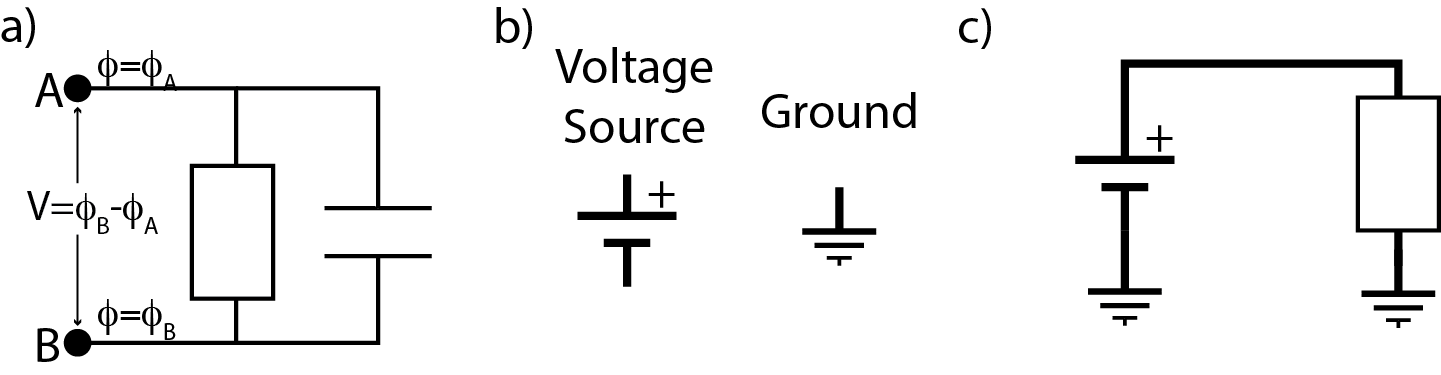
\includegraphics[width=\textwidth]{volt_ref}
\end{center}
\end{figure}

An ideal voltage source is something (anything) which can maintain a fixed electric potential between two points. What is meant by a non-ideal source will be discussed next lecture. Note that we don't care how it is made - it could be a battery, solar generator, or bench-top power supply. We draw an ideal voltage source, regardless of its construction as in figure \ref{fig:volt_ref}b. We thus arrive at our first layer of abstraction, and will continue to replace complicated devices by little cartoon which simplify design significantly throughout the course.

A key concept is that of electrical ground, often called \textit{ground}, or ``earth''. Since voltages are always defined with respect to a reference voltage, a given point in a circuit is often denoted as the 0V point, against which all other measurements are made. Ground in a circuit is so important that it is given a special symbol (figure \ref{fig:volt_ref}c. 

\begin{figure}
\caption{(a) A ground connection outside some house in Australia (Wikipedia CC license) (b) All ground points in a circuit are connected.}
\label{fig:ground_ref}
\begin{center}
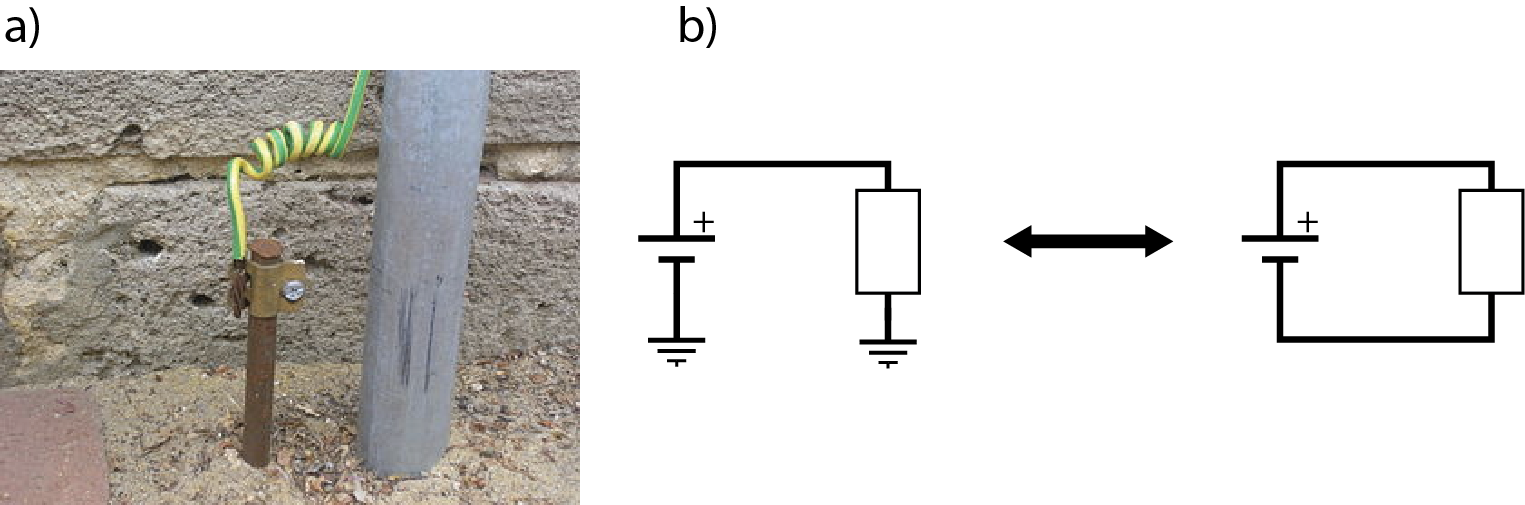
\includegraphics[width=\textwidth]{ground_and_pound}
\end{center}
\end{figure}

The name ground is quite literal -- it is often connected to a large stake driven into the Earth (fig. \ref{fig:ground_ref}a. The reason for this is that the (literal) ground provides a very large neutral body which whose potential will not change even when large amount of current are flowing into it. This would not be the case for a small metal plate which would develop a large charge imbalance and thus acquire a positive voltage. It is important to note that although not explicitly drawn, all ground connections are connected as if by a physical wire. 

The potential of the dirt outside your window need not be the reference voltage for $V=0$. Devices powered by a battery are clearly not connected physically to earth ground. Such devices are said to be \textit{floating} and the ground is often defined as the negative terminal of the battery. The term floating means that while the voltage \textbf{differences} are well defined along the circuit, their \textbf{absolute value} compared to an external reference are not and thus the ground level of two separate devices may float around with respect to one another. This can cause a significant danger when two floating devices are connected: since they do not have a common value for ground, high potential differences between the two devices can exist which will damage the device. 

\section{Wires, conductors, and insulators}
Just as masses in a gravitational potential will tend to accelerate to the lower potential, so to will current flow from a higher to a lower potential. To do so however, they charges need a path. As electrons are typically bound to their atoms via the coulomb force, they are typically sitting in their own potential well. This is why current isn't spontaneously flowing from one terminal of a battery to the other despite having a potential difference. Note however that if a sufficiently strong voltage is applied current will flow - even in vacuum. Certain materials however have electronic structure such that an individual electron is not bound to a particular atom and is free to move along an atomic ensemble, as long as it is replaced by another. These materials, known as conductors form the basis of electronic conductors. As long as one conductor maintains good contact with another, current may flow freely between them. The ease by which current flows is parametrized by the \textit{conductance} $\rho$ and has units of Siemens per meter.

At the opposite end of the spectrum are insulators which have electronic structure such that all electrons are tightly bound, giving them a very low conductivity. Insulators are as important as conductors in electronics as they provide the ``walls'' which keep current from flowing everywhere. It turns out that there is a third class of material we will deal with in this course which is somewhere in between a conductor and an insulator. Such a substance is known as a semiconductor. What makes semiconductors useful is that their conductivity can be easily tuned by introducing impurities and can by manipulated by injecting charges in between two different semiconductors. We will examine semiconductors in detail later in the course. Table \ref{tab:conduct} gives an overview of the conductivity of various materials.

\begin{table}[]
\centering
\caption{Electrical properties of various materials}
\label{tab:conduct}
\begin{tabular}{lll}
\hline
Material    & Classification & Conductivity {[}S/m{]} \\ \hline\hline
Copper      & Conductor      &          $5.96\times10^7$             \\
Aluminum        & Conductor      &             $3.50\times10^7$           \\
Hard Rubber        & Insulator      &             $1.0\times10^{-14}$      \\
Quartz        & Insulator      &             $1.30\times10^{-18}$           \\
 Silicon & SemiConductor      &          0.01 -- 1000 [depending on doping]            \\ \hline
\end{tabular}
\end{table}

Wires form the basis of our next idealization/abstraction. Although wire contain a complex lattice of various atomic structure we treat them in our circuit as perfect conductors of electricity which allow us to instant transfer an electric potential from one place in a circuit to another (i.e. lines of equipotential). In a circuit diagram we draw them as lines and in our conceptualization, we think of them as ``electricity pipes'' which current flows though without resistance. 


\section{Resistors and Resistivity}

The conceptualization of current carrying wires as pipes leads to an oft-used and useful analogy in electronics: we can visualize the flow of charge as we would the flow of water through a pipe as sketched in figure \ref{fig:water_analogy}. In this analogy voltage sources are replaced with hydraulic pumps and potential differences are pressure differences and current is fluid flow. The conductivity is given by the pump width. 

\begin{figure}[h]
\caption{In the Hydraulic analogy, voltage sources are pumps, voltage is pressure, and resistance is pipe constriction.}
\label{fig:water_analogy}
\begin{center}
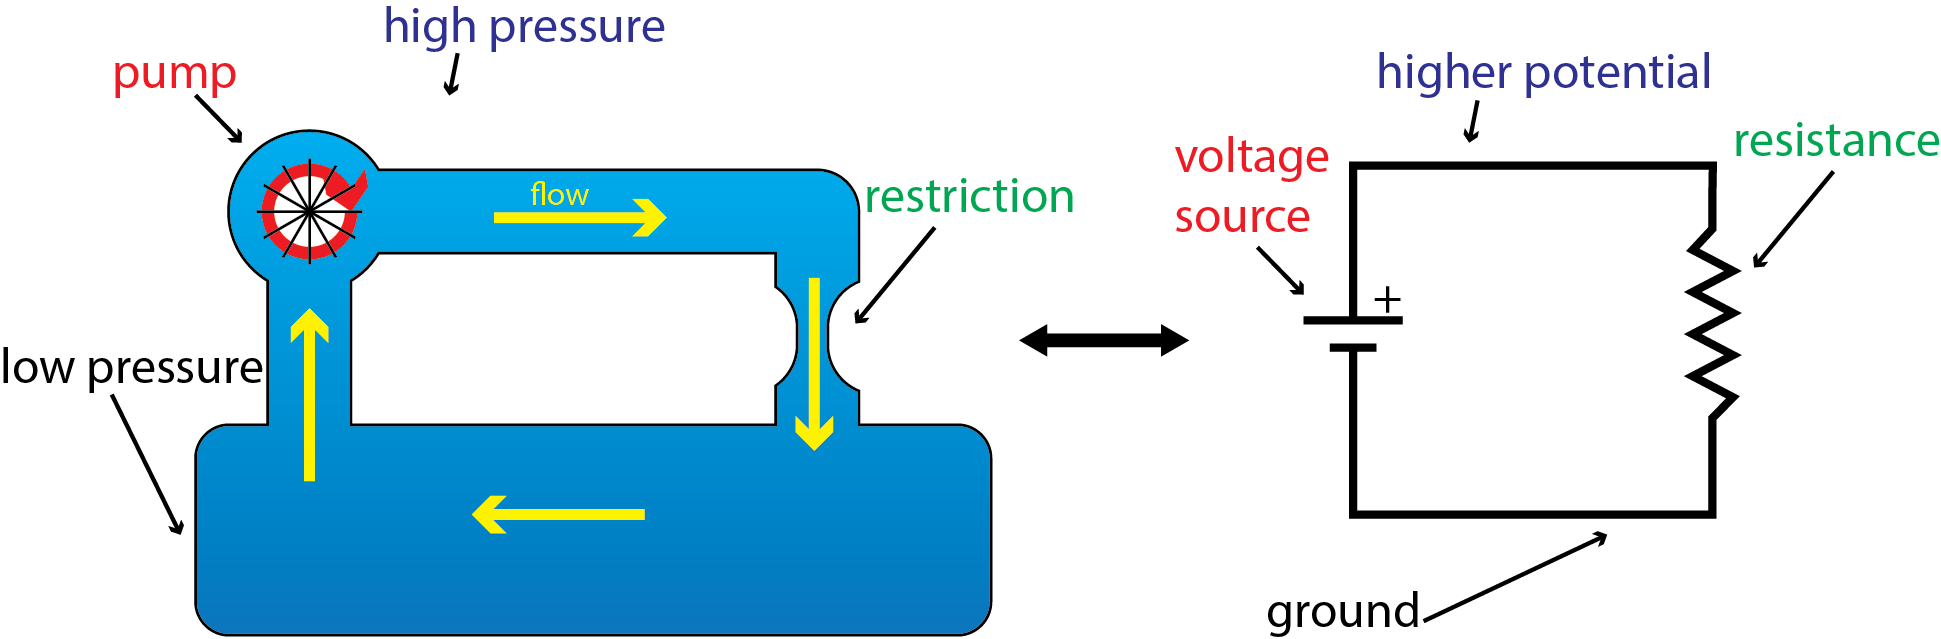
\includegraphics[width=\textwidth]{waterpumpanalogy.png}
\end{center}
\end{figure}

As you may imagine from the above analogy a wide, short wire will have an easier time passing current than  long thin one, which indeed turns out to be the case. The ease with which a given circuit element passes current for a given voltage is known as the resistance, defined as:

\begin{equation}\label{eq:def_res_op}
R \equiv \frac{V}{I}
\end{equation}

It turns out that for a conductor, the resistance can be determined from its geometry and conductivity, or as is most often used, its inverse -- the resistivity:

\begin{equation}\label{eq:def_resistivity}
\rho \equiv \sigma^{-1}
\end{equation}

Specifically, for a wire with resistivity $\rho$, cross sectional area $A$ and length $L$, the resistance is given by:

\begin{equation}\label{eq:def_resistance}
R = \rho\frac{L}{A}
\end{equation}

Consistent with the water analogy the longer the wire, the higher the resistance, but this can be compensated by increasing its area (think of blowing through a long stir stick vs. a giant bubble tea straw -- which is harder?).

For certain circuit elements the ratio in equation \ref{eq:def_res_op} is constant for all voltages. These devices are said to be ``Ohmic'' and obey \textit{Ohm's Law}.

\begin{equation}\label{eq:ohmslaw}
  \boxed{V = IR}
\end{equation}

\noindent  \textcolor{red}{\textbf{WARNING}}: many circuit devices are non-ohmic and do not satisfy Ohm's law. In some texts, Ohmic just means a resistor, and non-Ohmic means anything else. To go further, \textbf{nothing} in nature is truly Ohmic since nothing is truly linear, but for Ohmic materials, the nonlinearity is so small that the point is moot. Whether or not a device is Ohmic can be determined by plotting voltage as a function of current by means of a so-called ``IV curve''. An IV curve for a resistor and for a non-Ohmic device is shown in figure \ref{fig:ohmic}.

\begin{marginfigure}%
  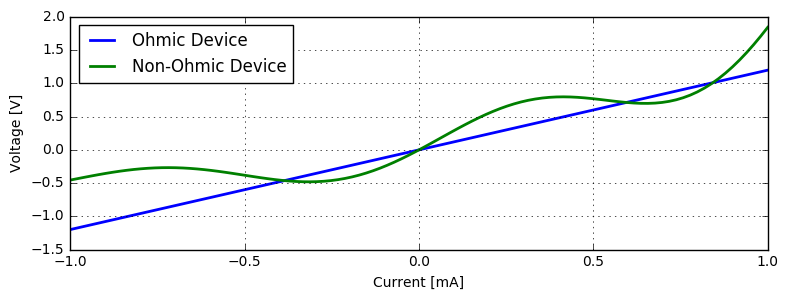
\includegraphics[width=\linewidth]{ohmicnonohmic}
\caption{Many devices are non-ohmic. The ratio of voltage to current is constant for resistors (blue) which obey Ohm's law. Other materials are non-Ohmic and have a non-constant slope (green) }
  \label{fig:ohmic}
\end{marginfigure}


Resistors are constructed by taking a conductor with a given resistivity $\rho$ and very carefully tuning the geometry to create a well defined resistance via equation \ref{eq:def_resistance}. There are several design techniques: wire-wound resistors are made by taking a very thin wire and wrapping it around a coil until a desired length - and thus resistance is achieved. Thin film resistors take an opposite approach and tune the area of a fixed length film via the thickness. In either case the resistors are encases by an insulating material and placed in a compact package. Conducting leads allow the resistor to connect to other circuit elements. Figure \ref{fig:someresistors} displays some of the existing technologies.

\begin{marginfigure}%
  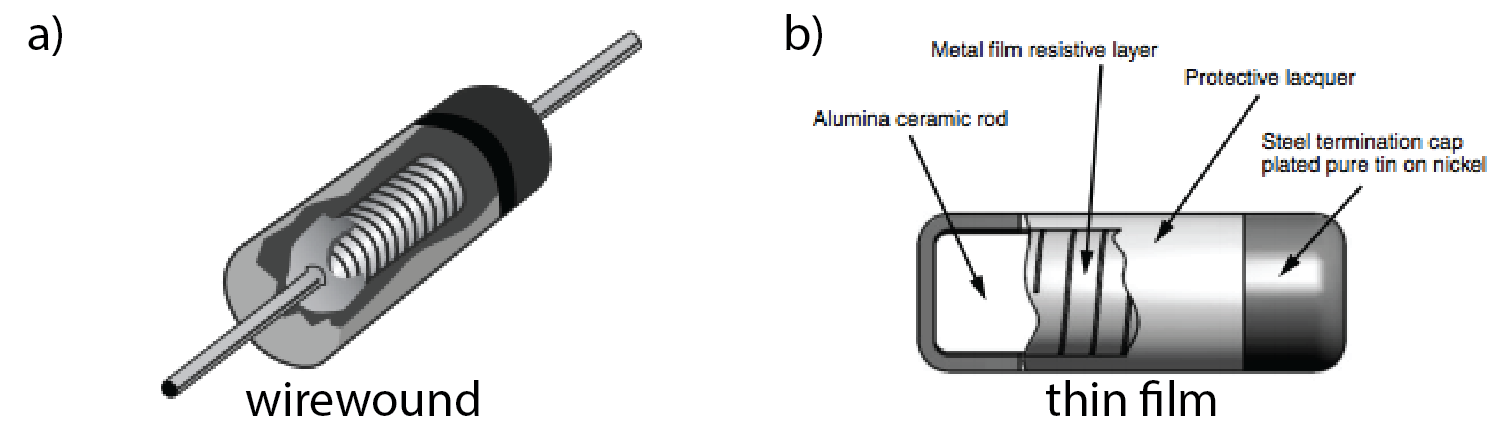
\includegraphics[width=\linewidth]{someresistors}
\caption{Sketch of a wirewound (a) and thin-film (b) resistor. Image from Vishay application note 28771}
  \label{fig:someresistors}
\end{marginfigure}

You may also notice colored rings on the resistors you use in the lab. This is the resistor color code that allows you to determine the resistance by cross-referencing with a look-up table. Such a table is included in the manual of Lab 1.  Some gurus may take pride in memorizing the resistor color code and can tell you that you are holding a 12~k$\Omega$ resistor just by looking at it.

There are also variable resistors known as potentiometers which you will become familiar with in the lab. These work by having a moving conducting terminal which can slide along the resistor, continuously changing the length and therefore via eq. \ref{eq:def_resistance}, the resistance.


\subsection{Resistance of Non-Ohmic Devices}
\newthought{Note the} distinction between equations: \ref{eq:def_res_op} and \ref{eq:ohmslaw}. The latter implies that there is a linear relationship between voltage and current, and the ratio is the resistance. Equivalently, when plotted on an IV curve, the slope of the plot is the resistance.

This leads to two generalizations of resistance as either the ratio or the slope:

\begin{subequations}
\begin{align}
    R_{s} = \frac{V}{I}\label{eq:genres1}\\
   R_d = \frac{dV}{dI} \label{eq:genres2}
\end{align}
\end{subequations}

The quantity $R_s$ is known as the ``static resistance'' and $R_d$ is the differential resistance. Note that unlike static resistance which is necessarily positive, the a device can have negative differential resistance, meaning that $R_s$ decreases with increasing current. The regions $-0.7\text{ mA}  < I < -0.3\text{ mA}$ and $0.4\text{ mA}  < I < 0.7\text{ mA}$ in figure \ref{fig:ohmic} display this.

One common example of negative differential resistance is the fluorescent light bulbs which are installed in most office buildings. As more current flows, the bulb becomes more conductive. To circumvent a runaway process in which more and more current is drawn until a catastrophic failure (i.e. explosion) occurs, fluorescent lights are powered by ``ballasts'' that switch the current at high frequencies. In lab 10, you will construct an optical sensor to measure this switching frequency.


\subsection{Electrical Power and Joule Heating}
Ohms law tells us that when current flows through a resistor there is a drop in voltage and therefore a drop in the energy of each charge in the current. Given that energy is conserved, where does this energy go? It turns out that on the microscopic scale, the electrons comprising the current undergo inelastic collisions with the lattice of the material. It is just the likelihood of these elastic collisions which determine the conductivity/resistivity of the material. 

Recall that in an inelastic collision, the particles lose kinetic energy and it this is just the case here. The electrons are accelerated by being in an electric potential until they collide with an ion in the lattice and bounce off, with less kinetic energy than they had before. Since the lattice ions are fixed, all of their motion goes into vibrations and we know this random atomic-lattice vibration as heat. This effect is known as \textit{Joule Heating}.

As the electrons are dumping a given amount of energy per unit time due to the current, this heating is a power having units of Watts (1W = 1J/s). The general expression for the heating due to a current $I$ across a potential difference $V$ is remarkably simple, and is given by:

\begin{equation}\label{eq:joule_gen}
\boxed{P=IV}
\end{equation}

For Ohmic materials, we can use Ohm's law to re-write this solely in terms of voltage and resistance:

\begin{equation}\label{eq:joule_ohm}
P = I^2R = \frac{V^2}{R}
\end{equation}

This is actually how incandescent light bulbs work. They they are formed by a thin wire having a non-ohmic resistance\footnote{The reason that the wire here is non-ohmic is that it heats up considerably which leads to more collisions and thus higher resistance} and the Joule effect causes them to heat up until they glow white-hot. Older light bulbs are thus simply heaters that get so hot they happen to glow. They are also remarkably inefficient -- only about 2\% of their power is converted into visible light. A modern white-light LED on the other hand can reach nearly 50\%.



\begin{myexample}[label = ex:res_lightbulb]{The resistance of a 60W light bulb}
A 60W light bulb means that at wall-voltage (120V) the filament can safely absorb 60W of heat. What is the current of the light when operating at 60W? What is the static resistance?
\Solution % uncomment for solution style
From equation \ref{eq:joule_gen}, we see that $I = P/V = 60W/120V = 0.5A$. Thus we see that a current of 500 mA is drawn. The (static) resistance is then 
$$
R_s = V/I = 120V/0.5A = 240 \Omega
$$
\end{myexample}



% \noindent\textbf{Pop Quiz}:

% \noindent(a) Does the current increase/remain equal/decrease? 

% \noindent(b) Is the resistance higher/equal/lower? 


\section{Connecting resistors}
A real circuit does not typically contain a single battery pushing current through a single resistor. There is a network of resistors, and other components which we will learn about shortly. When resistors are connected together they simply form a new resistor of a different resistance. Since resistors are two-terminal devices, it turns out that there are only two basic ways that a pair of resistors can be connected:

\begin{figure}[h]
\caption{Sketch of Series and parallel connections}
\label{fig:res_series_parallel}
\begin{center}
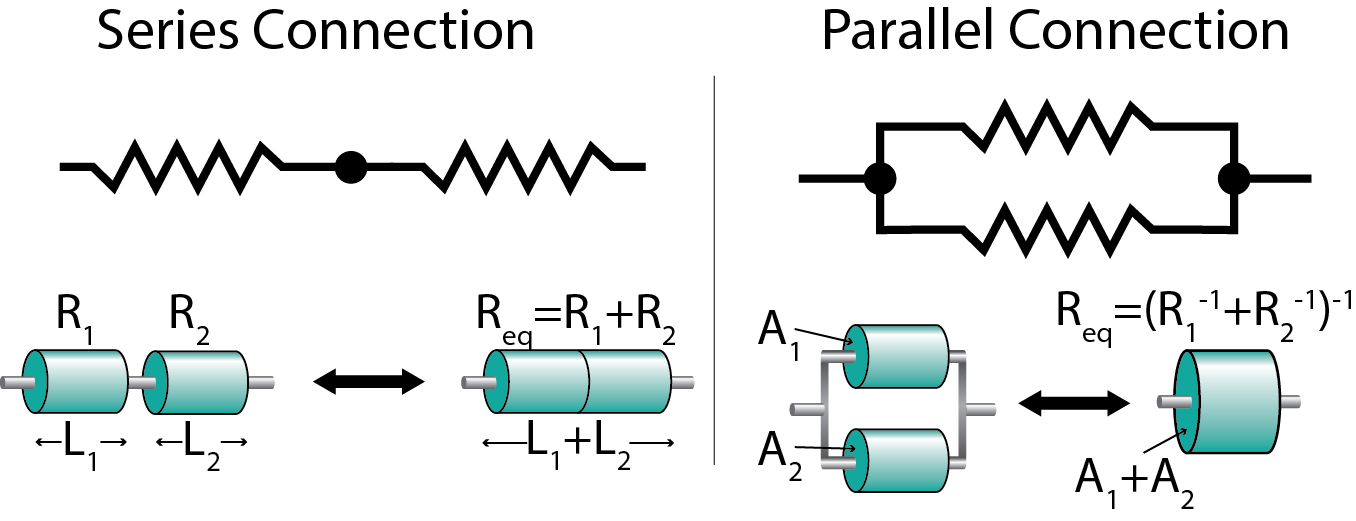
\includegraphics[width=\textwidth]{res_series_parallel.png}
\end{center}
\end{figure}


\subsection{Series connection} In a series connection the resistors are placed end to end and all of the current is forced to flow through both resistors. The voltage drop is split between the two resistors. Referring to figure \ref{fig:res_series_parallel}, we see that this is equivalent to increasing the length of the resistor and thus the resistance increases. To understand this more quantitatively, consider two resistors of equal area $A$ and lengths $L_1$ and $L_2$ such that the resistances are $R_1$ and $R_2$ given equation \ref{eq:def_resistance}. Connecting them in parallel then leads to a new resistor with length $L = L_1 + L_2$ with resistance $R = \rho\frac{L}{A} = \rho\frac{L_1}{A} + \rho\frac{L_2}{A} = R_1 + R_2$.  This is true in general:

\begin{equation}\label{eq:series_res}
\boxed{R_{\text{series}} = R_1+R_2}
\end{equation}

\subsection{Parallel connection} In a parallel connection, the current is split between two resistors but the voltage drop is the same across both since they are connected to a common node. From the figure we see that two resistors in parallel are equivalent to a single resistor with greater area. The resistance of a series connection is thus less than that of its constituent resistors. To get more quantitative again, consider two resistors with equal length $L$ and resistivity $\rho$, but different areas $A_1$ and $A_2$, yielding resistances $R_1$ and $R_2$. The resistance of the parallel connection is given by $R = \rho\frac{L}{A} = \rho\frac{L}{A_1+A_2}$. Therefore we have: $R^{-1} = \frac{A_1+A_2}{\rho L} = \frac{A_1}{\rho L} + \frac{A_2}{\rho L} = R_1^{-1} + R_2^{-1}$. We thus arrive at the equivalent resistance of a parallel resistance:

\begin{equation}\label{eq:series_par}
\boxed{R_{\text{parallel}} = \left(R_1^{-1}+R_2^{-1}\right)^{-1} = \frac{R_1R_2}{R_1+R_2}}
\end{equation}

\textbf{An Important Approximation:} In many cases in practice, a series or parallel combination is completely dominated by one of the two resistors. Consider two resistors: $R_1 = 10\text{ k}\Omega$ and  $R_2 = 50\text{ }\Omega$. The parallel combination of the two gives $R_{\text{series}} = 10$ k$\Omega$ + $50\text{ }\Omega = 10.05\text{ k}\Omega \approx 10\text{ k}\Omega$. On the other hand, the parallel connection gives $ R_{\text{parallel}} = \frac{50\Omega\times10^4\Omega}{10050\Omega} = 49.751\ldots \approx 50\Omega$. 

\noindent Thus if $R_1\gg R_2$, the series combination gives $R = R_1 + \epsilon$ and the parallel combination gives $R = R_2-\epsilon$ where $\epsilon/R\ll1$.

More complicated combinations of resistors can always be reduced to an equivalent resistance. An example is given in figure \ref{fig:ex_resnet}. First, we see that the two 1k\footnote{``In the shop'', you rarely take the time to say ``kilo-ohm'' but say ``kay'' instead. Lazy, I know, but that's how it is.} resistors in the top are just a series combination, equivalent to a single 2k resistor. This gives a parallel combination of two 2k resistors which is equivalent to a single 1k resistor. Finally, we are left with a series connection of 2 1k resistors, so that the entire circuit is equivalent to a single 1k~$\Omega$ resistor.

\begin{figure}[h]
\caption{Example resistor network reduction.}
\label{fig:ex_resnet}
\begin{center}
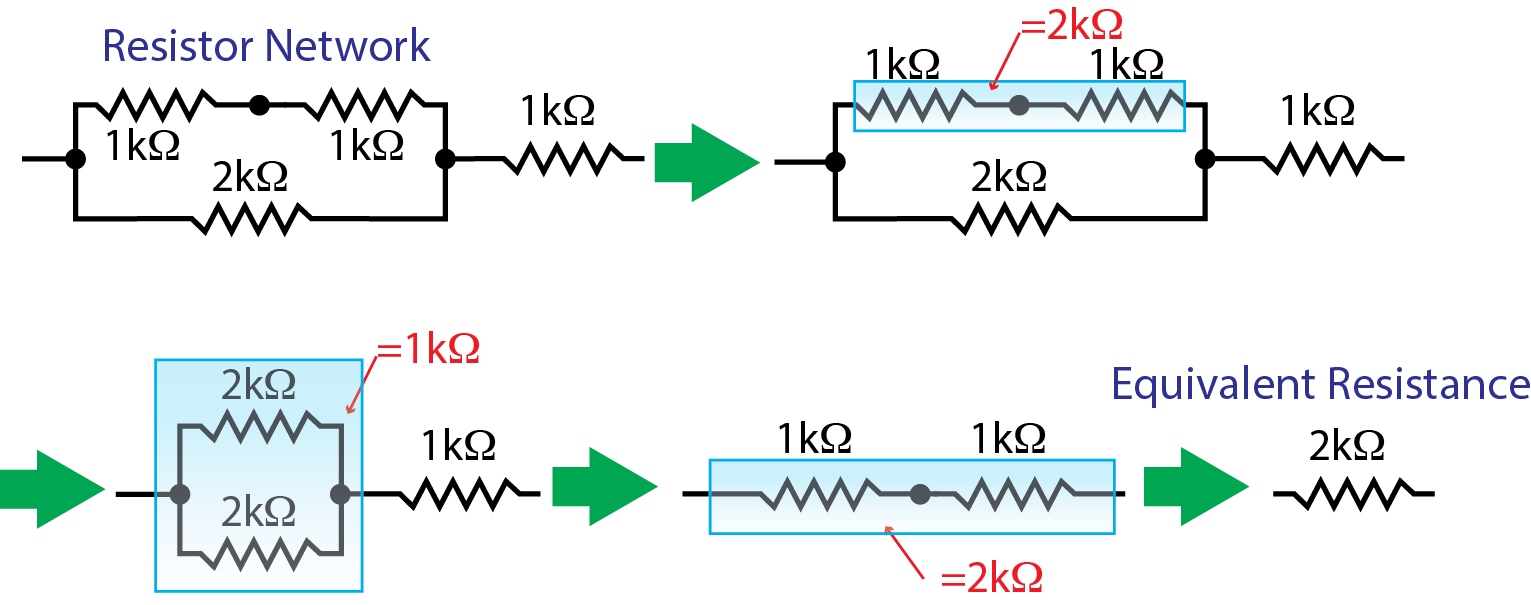
\includegraphics[width=\textwidth]{ex_resnet.png}
\end{center}
\end{figure}



%%% ========================================================================

\chapter{Circuit Analysis Fundamentals}
Now that we have an understanding of the fundamental components that make up a circuit, we can start designing and analyzing electronic circuits. The simplest circuits we'll look at are formed by connecting voltage sources and resistors with wires to form closed loops. This results in current flowing through resistors, and thus, according to equation \ref{eq:joule_ohm}, power is delivered to various elements in the circuits. So what do we mean when we say ``analyze a circuit''? We ``solve'' a circuit by determining the voltage dropped across, current running through, and power dissipated within, any to points in the circuit. The following sections go through the basic techniques.

\section{Elementary Circuit Analysis: An example}
\label{sec:circuitanalysis}
We can now use Ohm's law, along with the equations for parallel and series resistors to completely analyze a circuit. Not all circuits can be analyzed this way and for those, we will need a new method known as Kirchhoff's rules. 

\begin{figure}[h]
\caption{Elementary circuit analysis}
\label{fig:elemcirc}
\begin{center}
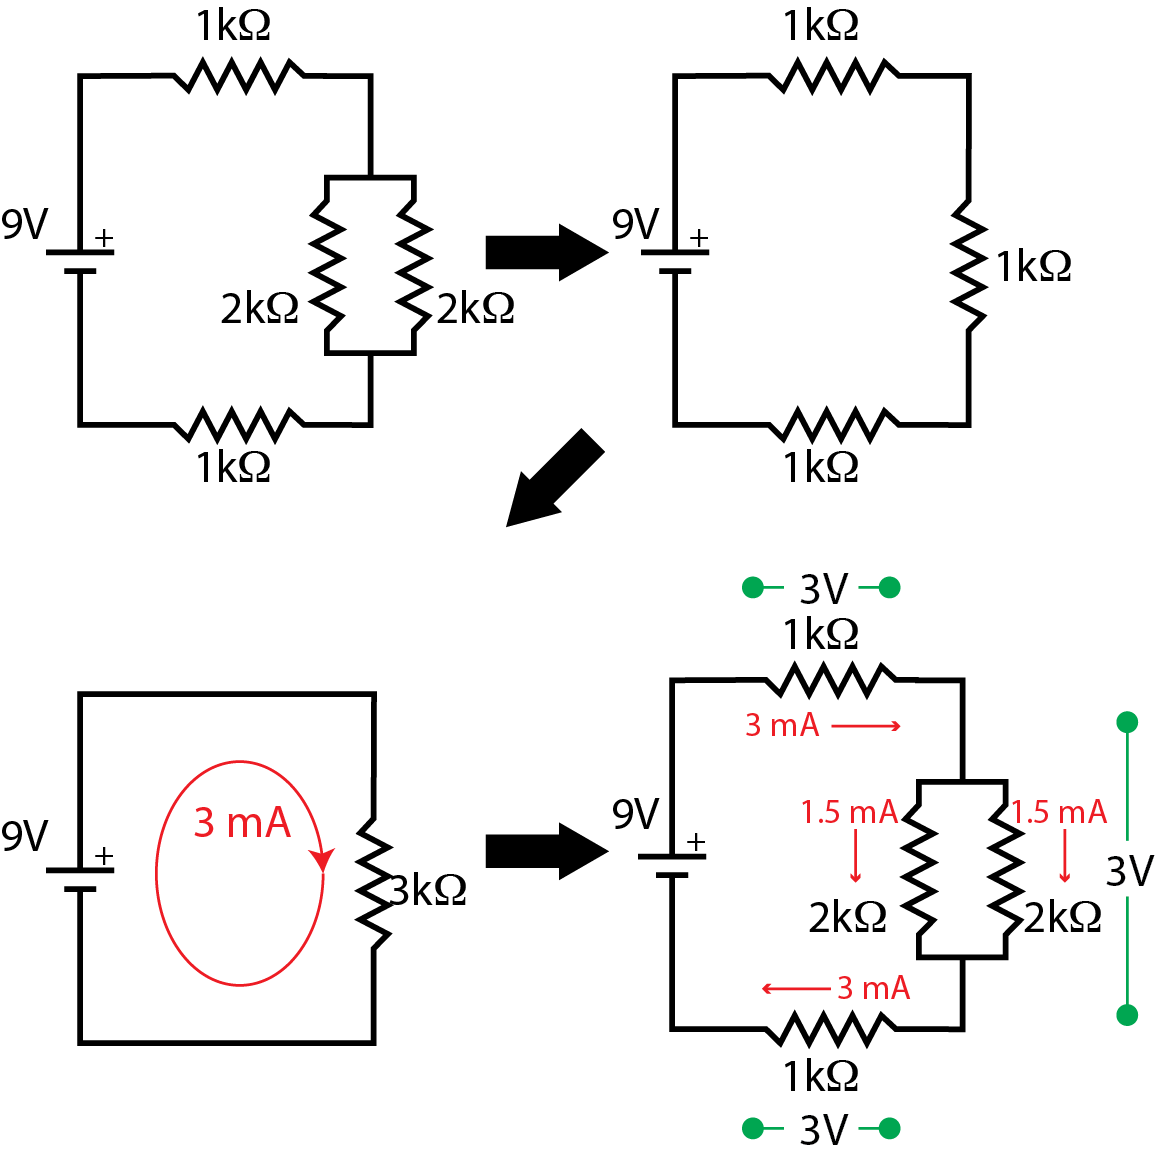
\includegraphics{elemcirc.png}
\end{center}
\end{figure}


Consider the circuit in figure \ref{fig:elemcirc}. Our goal will be to slowly fill in all the voltage drops and currents in this circuit and know all that there is to know about the circuit. 

\begin{myexample}[label = ex:elem_circuit_anal]{Analysis of circuit in figure \ref{fig:elemcirc}}
We can take a forward--backward sweep approach. What I mean is that we first reduce the resistors in the circuit so that we are left with the ultra simple circuit in figure \ref{fig:elemcirc}c. This gives us the current supplied by the battery. Knowing the current we can use Ohms law to find voltage drops across the series resistances, which let's us determine the current through individual parallel combinations. Don't worry -- it's easier done that said:\\
\textbf{Step I} Reduce the parallel combination ($a\rightarrow b$). From the rules for parallel resistors, we see that these two 2~k$\Omega$ resistors are equivalent to a single resistor with $R = \left((2~\text{k}\Omega)^{-1} + (2~\text{k}\Omega)^{-1} \right)^{-1} = 1~\text{k}\Omega$.\\
\textbf{Step II} Reduce the remaining parallel resistors into a single battery, single resistor circuit ($b\rightarrow c$). We have 3 1~k$\Omega$ resistors in series, equivalent to a single 3~k$\Omega$ resistor. When connected to a 9~V battery, this gives a current of 3~mA.\\
\textbf{Step III} Work backwards and determine everything about the circuit ($c\rightarrow d$). We see the voltage drop across the parallel resistors and the two 1~k$\Omega$ resistors is $V = IR = 3~\text{mA}\times1~k\Omega = 3~\text{V}$. The current through the 2~k$\Omega$ resistors is $I=V/R = 1.5~\text{mA}$ and we know all there is to know about this circuit.
\end{myexample}

\section{Measuring DC quantities: The Digital Multimeter}
\subsection*{The Digital Multimeter (DMM)}
A voltmeter is a device that measures the potential difference across two points on a circuit when placed in parallel across the two points. Similarly, an ammeter measures current through a wire by inserting itself in series with the wire. An ohmmeter measures the value of a resistor. 

Thankfully there is a very common device known as a digital multimeter (DMM) which does all three - and more. The ``digital'' part of it means that the continuous (or analog) quantities measured are converted into digital format via an aptly named \textit{analog to digital converter} or ADC which we will study later in the course. You will use make heavy use of a DMM in every one of your labs. The procedure for the 3 basic measurement are described as follows:

\subsection*{Voltage}






\begin{figure}[h]
\caption{Measuring Voltage}
\label{fig:measvolt}
\begin{center}
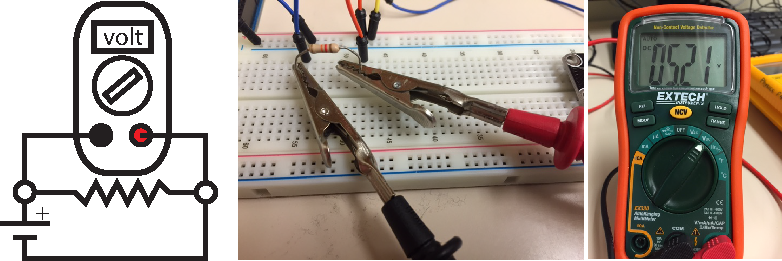
\includegraphics{DMM_voltage_meas.pdf}
\end{center}
\end{figure}

When measuring \textbf{voltage} between two points on a circuit, first ensure your probe ends are connected to the correct inputs of the Digital Multimeter (DMM) for measuring a DC voltage, and that the voltage setting is selected.
Probe tips can then be placed in parallel across the circuit (Fig.~\ref{fig:measvolt}). 
The circuit does not need to be modified for this measurement, making voltage measurements relatively straightforward.
From voltage measurements and known resistances, the current through the circuit can be inferred from Ohm's law, however the DMM can be configured to measure resistance and current directly.

\subsection*{Current}

In contrast to voltage measurements, \textbf{current} measurements are performed in series along the circuit.
First ensure your probe ends are connected to the correct DMM inputs for measuring current.  
When you connect your probe tips, it is essential that the DMM is wired in series with the current being measured.  
If it is properly wired in series, the current will be forced to flow through the DMM (Fig.~\ref{fig:meascurr}) and a measurement can be made.

\textbf{Warning:} The DMM measures current by measuring the voltage dropped across a calibrated resistor of very small resistance. Measuring current in parallel will draw high current through the DMM and blow a fuse. \textbf{Do not measure current in parallel!}

\begin{figure}[h]
\caption{Measuring Current}
\label{fig:meascurr}
\begin{center}
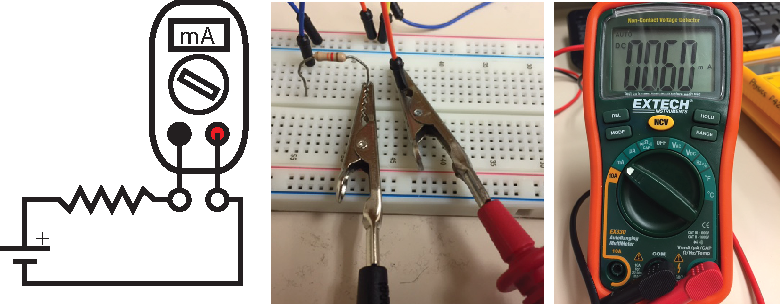
\includegraphics{DMM_current_meas.pdf}
\end{center}
\end{figure}

\subsection*{Resistance}

When measuring \textbf{resistance}, it is important to isolate the resistor in question (i.e. remove it from the circuit) as shown in Fig.~\ref{fig:measres}. 
If left connected, the DMM measures the series connection of the resistor and the rest of the circuit. 
Ensure your probe ends are connected to the correct DMM inputs for measuring resistance. 

\begin{figure}[h]
\caption{Measuring Resistance}
\label{fig:measres}
\begin{center}
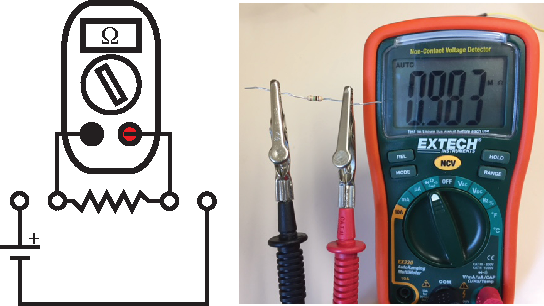
\includegraphics[width=0.7\linewidth]{DMM_resistance_meas.pdf}
\end{center}
\end{figure}

\section{Kirchhoff's Rules}\label{sec:kirchhoff}
Earlier, we saw that often, a nasty network of resistors such as in figure~\ref{fig:kirchhoff_circuits}a can be analyzed by reducing the constituent resistors via the rules of parallel and series combinations of resistors. Surprisingly, some seemingly simple circuits such as those in figure~\ref{fig:kirchhoff_circuits}b can not. Fortunately, there is an alternative approach to analyzing any circuit, using a very important set of relations known as Kirchhoff's laws.

\begin{figure}[h]
\caption{a) Some circuits can be reduced using parallel and series combinations of resistors, b) some can't}
\label{fig:kirchhoff_circuits}
\begin{center}
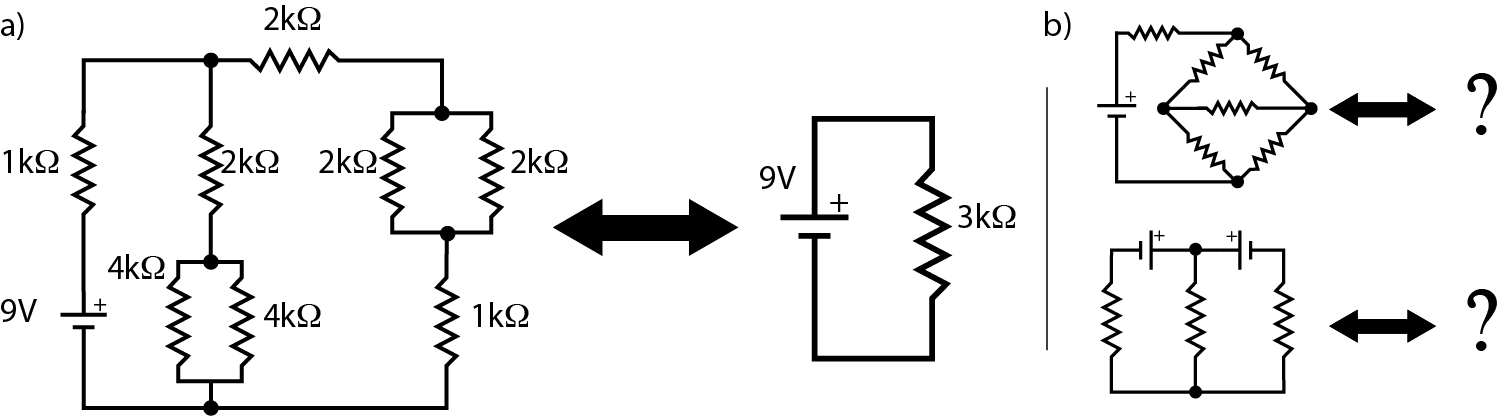
\includegraphics{kirchhoff_circuits.png}
\end{center}
\end{figure}


Kirchhoff's ``Laws'' are sometimes called Kirchhoff's rules because they are not law really \textit{laws} in the sense that Newton's Laws are laws. Rather, they are rules which are highly accurate when applied under a certain set of approximations which are consistant with the ``Good Circuit" Approximation''. I say this only because they seem to stem from fundamental physics such as the conservation of energy and of charge whereas this is not strictly true. \footnote{Specifically, Kirchhoff's laws hold in the so-called ``lumped element'' approximation. In this model, a resistor is like a point object with an nput and an output. In reality, the voltage and current can vary or even change direction withing the element. The element can also affect and be affected by other circuit elements through electric and magnetic fields even if there are no wires connecting them. This considerations typically become important at high frequencies, where electromagnetic readiation can be significant and where the inputs change faster than the time it takes the change to propagate throught the circuit.}

\subsection{Statement of Kirchhoff's rules}
Consider the simple circuit containing a battery, and a few resistors in figure \ref{fig:kirchhoff_deriv1}. 

\begin{marginfigure}%
  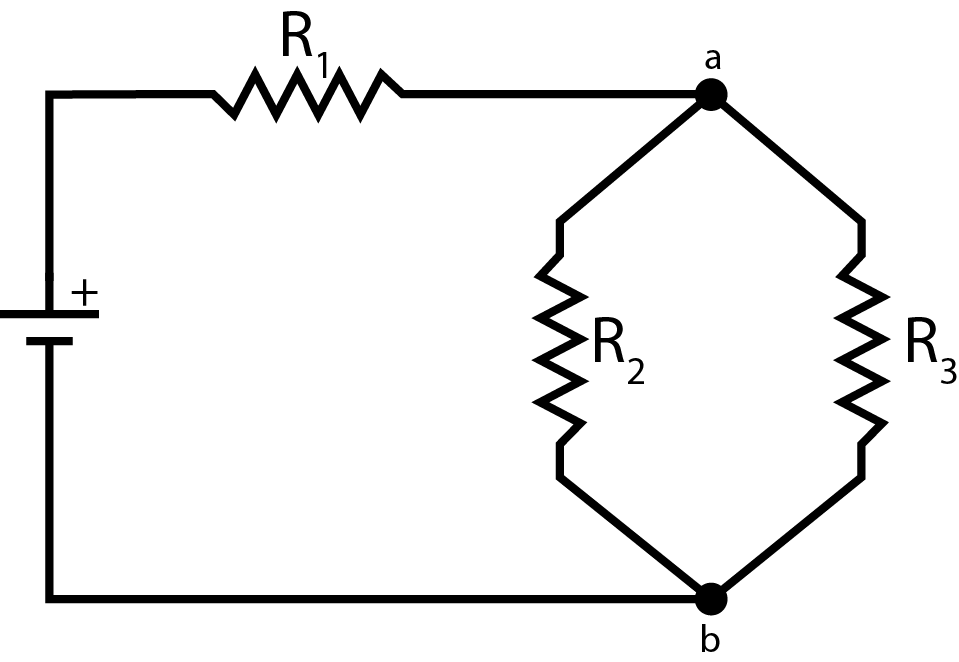
\includegraphics[width=\linewidth]{Kirchoff_I}
  \caption{Circuit with loops and nodes.}
  \label{fig:kirchhoff_deriv1}
\end{marginfigure}



In this particular circuit, we see that current will flow from the positive terminal of the battery, though resistors and into the negative battery terminal (figure \ref{fig:kirchhoff_deriv2}). What can we say about the current through resistors $R_2$ and $R_3$? Since current is due to a flow of individual charged particles, the total charge is conserved. Thus the current flowing into junction $a$ must equal the current flowing out of junction $a$. Denoting  current flowing into the junction as positive and current flowing out as negative, we have $I_1 = -I_2 + I_3$, or $I_1 + I_2 + I_3 = 0$.


\begin{marginfigure}%
  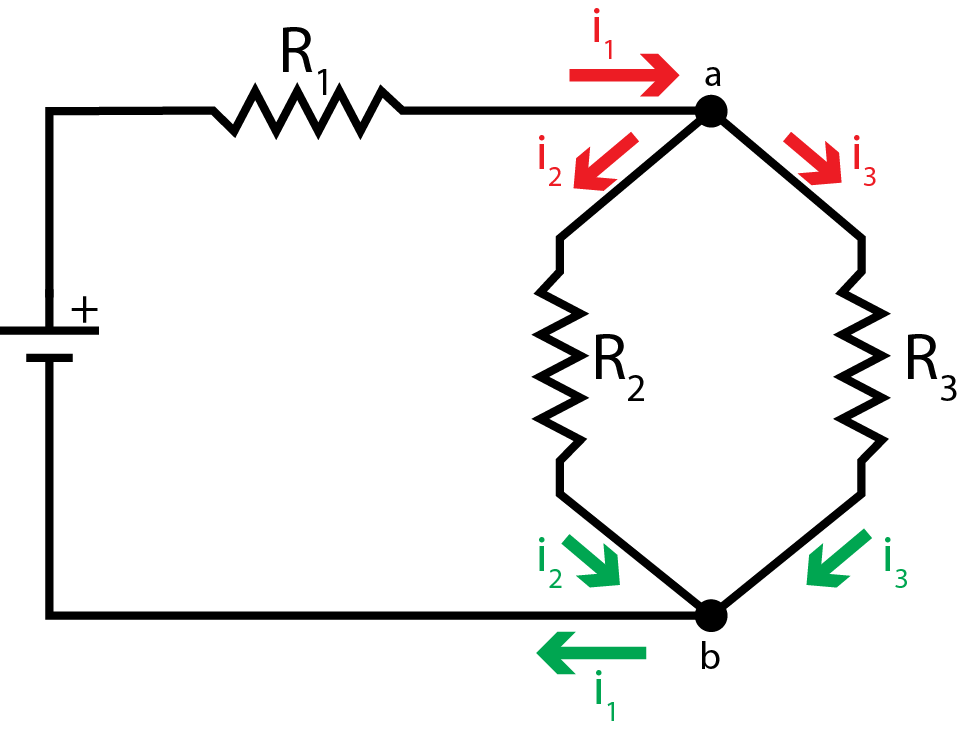
\includegraphics[width=\linewidth]{Kirchoff_III}
  \caption{Kirchhoff's Current Rule.}
  \label{fig:kirchhoff_deriv2}
\end{marginfigure}


This is a particular case of a general principle of conservation of charge, known as:

\noindent\textbf{Kirchhoff's First Rule:} \textit{The net current flowing into and out of any node in a circuit must be precisely zero}:

\begin{equation}\label{eq:Kirchhoff_I}
\boxed{\sum_kI_k=0}
\end{equation}

\noindent Note that since the current out of the battery must equal the current into the battery, analysis of the second node yields an identical result: $I_2 + I_3 = -I_1$.

Next we move on to a second rule. The EMF provided by the battery results in a potential difference $V_0$ which drives charges around the circuit. As the charge moves from the positive to the negative terminal it loses a potential energy $V_k$ at each resistor until it reaches 0~V at the negative terminal of the battery. Notice that we didn't say which path the charge took on its way around the circuit. The fact of the matter is that whether it took the outer or the inner loop (see figure \ref{fig:kirchhoff_deriv3}) the voltage dropped is always equal to the EMF provided by the battery: $V_\text{loop} = -V_0$, or $V_\text{loop}+V_0 = 0$. Moreover, consider a charge moving in a loop from node $a$, through 1 resistor to $b$ and back up through the other resistor to $a$. At each resistor, there is a change in voltage but since it arrives at the same point, the net voltage drop is zero. This is required by conservation of energy, for if the change in voltage is positive we would gain energy in each loop and could build a perpetual motion machine by repeating the loop \textit{ad infinitum}. If the change in voltage were negative, we could just reverse direction of the loop and repeat the same argument. 

Thus again: $V_{R1} + V_{R2} = 0$. These are particular examples of a general rule principle known as:

\noindent\textbf{Kirchhoff's Second Rule:} \textit{The net change of voltage around any closed loop must be precisely zero.}

$$
\boxed{\sum_kV_k=0}
$$

\begin{marginfigure}%
  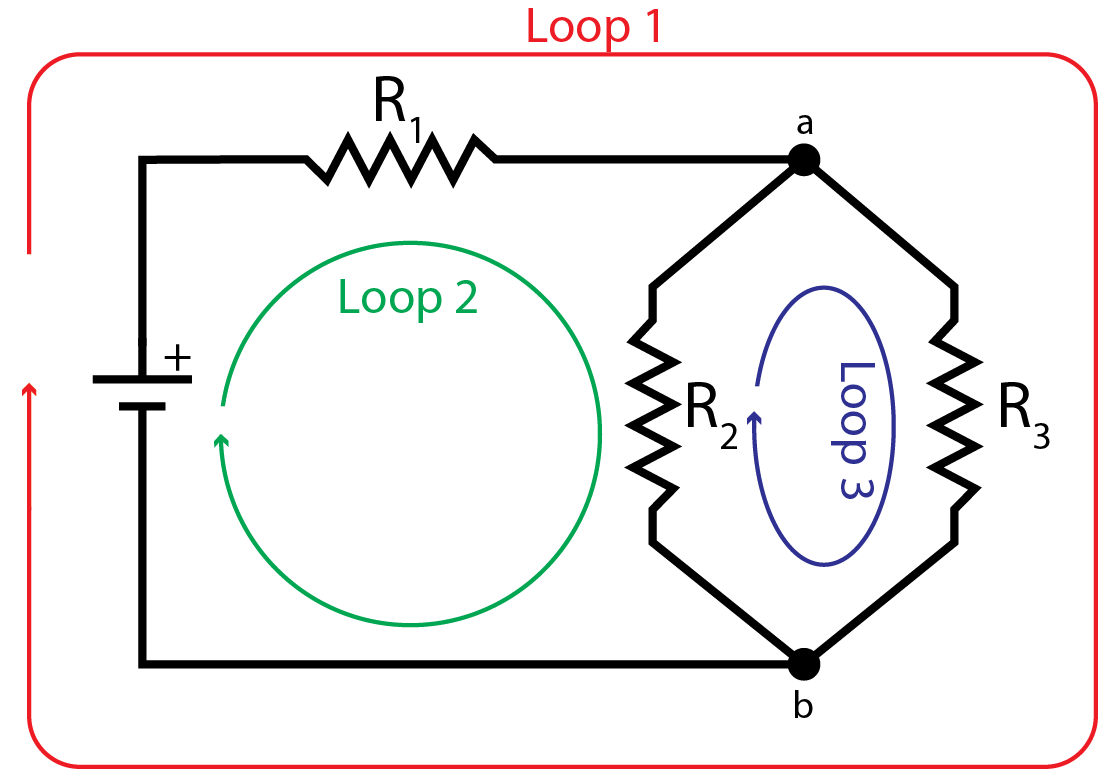
\includegraphics[width=\linewidth]{Kirchoff_II}
  \caption{Kirchhoff's Current Rule.}
  \label{fig:kirchhoff_deriv3}
\end{marginfigure}


\noindent Kirchhoff's rules will always allow you to reduce a circuit to a system of linear equations. When solving by hand, this often leads to much mathematical tedium and should be avoided if the circuit can be analyzed another way. However, it provides a good algorithmic approach which can be programmed into a computer to systematically solve circuits. Circuit simulation packages such as SPICE do just this. Disclaimer aside, we now provide a worked example. 
\\
\begin{figure}[h]
\caption{(a) The circuit we wish to analyze via Kirchhoff's Rules. (b) Setting up a current convention at node $b$. (c) Applying Kirchhoff's current and voltage rules.}
\label{fig:kirchhoff_ex}
\begin{center}
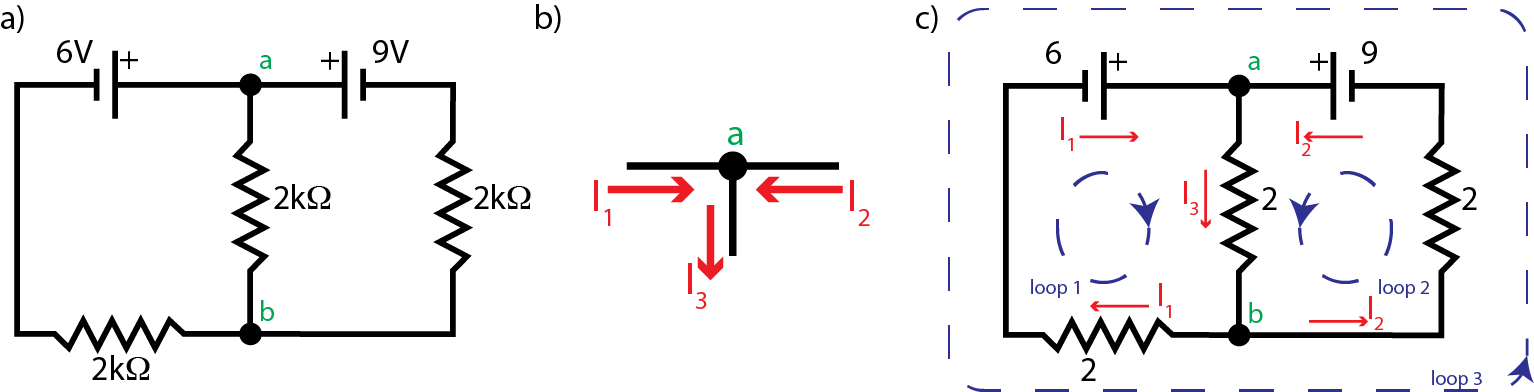
\includegraphics[width=\textwidth]{kirchoff_ex.png}
\end{center}
\end{figure}


\begin{myexample}[label = ex:when_kirchhoff_isvalid]{A high--brow view of the validity of Kirchhoff's Laws}
\textcolor{red}{\textbf{WARNING}}: Advanced material. NSFSY (not safe for second year).

\noindent\textbf{Approximation I: No electromagnetic fields outside the circuit elements (Lumped element approximation)}

In this case, we know from Maxwell's equations that

$$
\oint_\Gamma\textbf{E}\cdot d\textbf{l} = \frac{d}{dt}\iint_\Sigma\textbf{B}\cdot d\textbf{A} = 0
$$

Using the lumped circuit model, we can split the split the closed loop $\Gamma$ into the set of wire segments (see figure \ref{fig:when_kirchhoff_isvalid}), so that

$$
\oint_\Gamma\textbf{E}\cdot d\textbf{l} = \sum_k\int_{\Gamma_k}\textbf{E}\cdot d\textbf{l} \equiv \sum_kV_k = 0
$$

Hence the sum of voltage drops around any closed loop is zero. This can be seen as a conservation of energy, since there is no energy entering or leaving the circuit through electromagnetic fields.

\noindent\textbf{Approximation II: no charge accumulates at the terminals or nodes (low frequency and zero resistance wires)}

In this case since the number of electrons (not to mention holes) is conserved, zero accumulation implies that the charge in must equal the charge out, of any node (see figure). Really, this is a statement that (a) we have well defined nodes that act as infinitessimal points and (b) that have accounted for every possible current path. In this case,

$$
\sum_ki_k=0
$$

\noindent If we don't have ideal nodes with 0 capacitance (see next chapter), charge \textbf{can} of course accumulate for a short amount of time and KCL is not true.

\end{myexample}

\begin{figure}%
  \includegraphics[width=\linewidth]{kirchoff_highbrow}
  \caption{a) KVL is valid when $d\textbf{B}/dt = 0$. b) KCL is valid as long as no charge accumulates in a node and all conduction paths are accounted for.}
  \label{fig:when_kirchhoff_isvalid}
\end{figure}

Kirchhoff's Laws allow us to solve any circuit we might come across, but it can be much more tedious than the reduction technique of example \ref{ex:elem_circuit_anal}. Typically the strategy is split into two steps:

\begin{myexample}[label = ex:kirchhoff_calculation]{Example Circuit Analysis Using Kirchhoffs Laws}

We will analyze the circuit in \ref{fig:kirchhoff_ex}a by applying Kirchoff's rules. 

\noindent We start by assigning a current convention. The directions of current can be completely arbitrary as long as the circuit is self consistent. Referring it \ref{fig:kirchhoff_ex}b, we focus on node $a$ and define the three currents as $I_1$, $I_2$, and $I_3$. This defines the rest of the currents in the circuit as shown if \ref{fig:kirchhoff_ex}c. A non-self-consistent circuit would, for example have $I_2$ running from $b$ toward $a$. 

Having done this we can write Kirchhoff's current rule at node $a$ as:

\begin{equation}\label{eq:Kirch_ex1}
I_1+I_2 = I_3
\end{equation}

\noindent Note that corresponding for node $b$ is redundant and gives no extra information. This is a common feature in Kirchhoff circuit analysis.

We now move on to applying Kirchhoff's voltage law. There are three loops to consider:

\begin{eqnarray}\label{eq:Kirch_ex2}
6~\text{V} - I_3\times2~\text{k}\Omega - I_1\times2~\text{k}\Omega &=& 0 \nonumber\\
9~\text{V} - I_3\times2~\text{k}\Omega - I_2\times2~\text{k}\Omega &=& 0 \nonumber\\
9~\text{V}-6~\text{V} +I_1\times2~\text{k}\Omega - I_1\times2~\text{k}\Omega &=& 0 
\end{eqnarray}


\noindent Note that the sign of the voltage drop is positive for batteries and negative for resistors when going in the direction of the current and vice versa when going against the current. We now have 4 equations in 3 unknowns and again, are stuck with an over constrained system. We use the first and third equations. For brevity, the units are dropped and we work in units of k$\Omega$, so that current is in mA. The dividing the first equation by 2 and inserting equation \ref{eq:Kirch_ex1}, we have:

\begin{eqnarray}\label{eq:Kirch_ex3}
2I_1 + I_2 &=& 3 \\
-2I_1 + 2I_2 &=& 3 
\end{eqnarray}

\noindent Addind these equations yields $I_2 = 2$ mA, and reinserting this value yeilds $I_1 = 0.5$ mA. Finally, Kirchoff's current law gives $I_3 = 2.5$ mA:


\begin{empheq}[box=\fbox]{align}
I_1 &= 0.5~\text{mA}\nonumber\\
I_2 &= 2.0~\text{mA}\nonumber\\
I_3 &= 2.5~\text{mA}\nonumber
\end{empheq}

Note that we can now solve for the any other quantity in the circuit. For example the potential between nodes $a$ and $b$ is seen to be $V_{ab} = I_3R = 2~\text{mA}\times2~\text{k}\Omega = 4~\text{V}$.

\end{myexample}
\begin{figure}[h]
\caption{(a) The circuit we wish to analyze via Kirchhoff's Rules. (b) Setting up a current convention at node $b$. (c) Applying Kirchhoff's current and voltage rules.}
\label{fig:kirchhoff_example}
\begin{center}
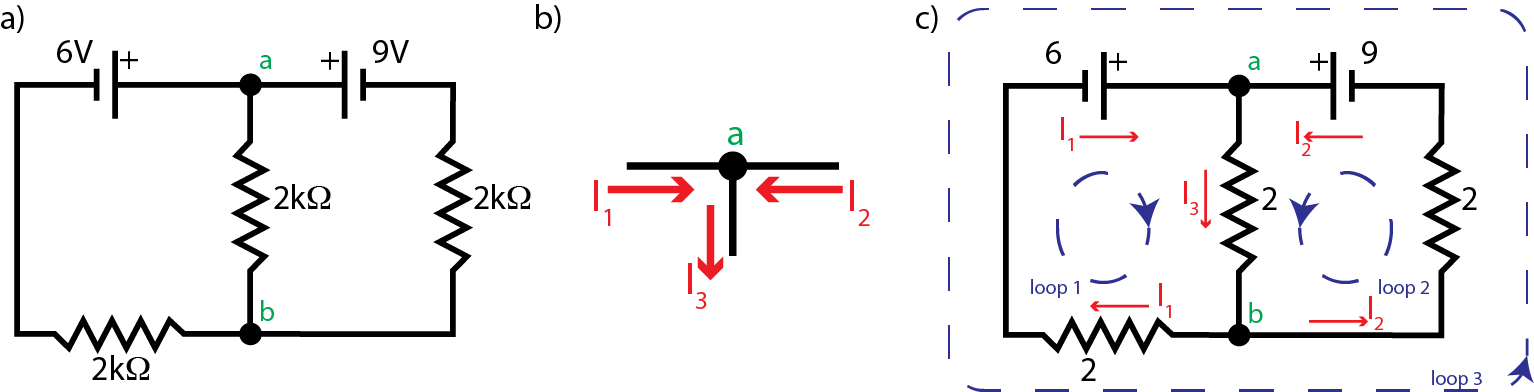
\includegraphics[width=\textwidth]{kirchoff_ex}
\end{center}
\end{figure}


\section{The Superposition Principle in Circuits}

Another way to solve the circtui ion example \ref{ex:kirchhoff_calculation} is to make use of the superposition principle, inherent to linear systems. In terms of electronic circuits, we note that since the electric potential obeys the superposition principle, we can think of the response of the system (i.e. the current resulting from the potentials) as the sum of all of the individual voltage sources acting at once. This is outlined in figure \ref{fig:superposition_circuits}. We look at the circuit when only the 6~V battery is applied and calculated the currents as in \ref{ex:elem_circuit_anal}. We do the same for the circuit when only the 9~V battery is applied. The resultant current is simply the sum of the currents in each case, for which we find a result consistent with example \ref{ex:kirchhoff_calculation}.

\begin{figure}[h]
\caption{Using the superposition principle in place of Kirchhoff's Rules to solve a circuit.}
\label{fig:superposition_circuits}
\begin{center}
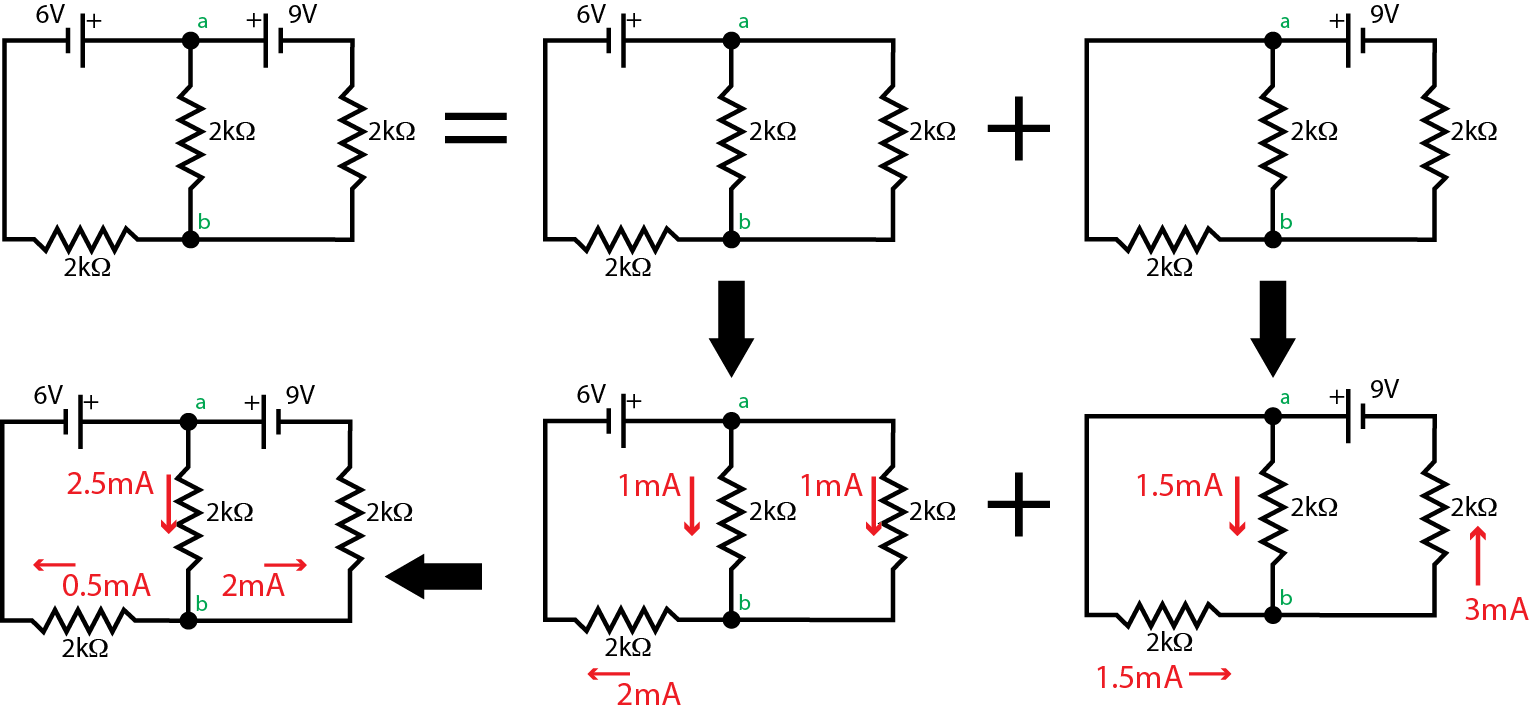
\includegraphics[width=\textwidth]{superposition_circuits}
\end{center}
\end{figure}


\section{The Voltage Divider}
Often, we want a particular voltage at a particular point in a circuit. For example, we may have an LCD screen which requires 3.3V in a circuit that is powered by a 9V battery. How might we accomplish this? The simplest-minded approach may be to just use a resistor to create a voltage drop as in figure~\ref{fig:voltagedivider}a. 


\begin{figure}[h]
\caption{(a) A bad way to make a voltage divider. (b) A good way to make a voltage divider. (c) Drawing too much current will affect performance of voltage divider.}
\label{fig:voltagedivider}
\begin{center}
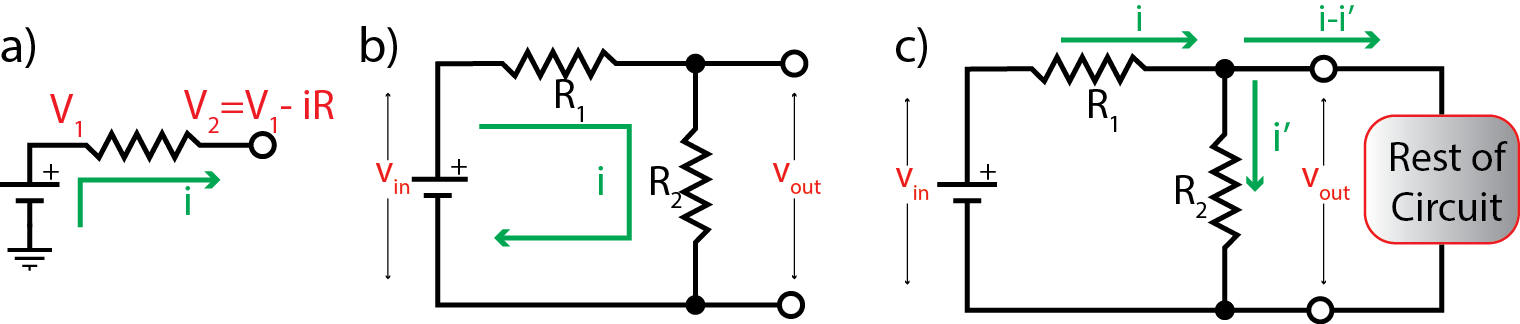
\includegraphics[width=\textwidth]{voltage_divider}
\end{center}
\end{figure}


By knowing the current of the circuit, we could work out what resistance required to drop the voltage to the desired value. However, as soon as the current changes based on fluctuations in temperature, other voltages, or whatever, the voltage will change. This voltage change may cause further fluctuations in current which will amplify the problem leading to a very unstable situation. 

So we can't make a good voltage converter with a single resistor, but surprisingly, we make one with two! Consider the circuit in figure~\ref{fig:voltagedivider}b. The total voltage drop across int the circuit is $V_{in}$ and the total resistance in the circuit is $R_{tot} = R_1 + R_2$. We then know the current going through the resistors from Ohm's law, to be: 

\begin{equation}\label{eq:vd_deriv1}
I = \frac{V_{in}}{R_{tot}} = \frac{V_{in}}{R_1 + R_2}
\end{equation}

Next, note that the output voltage is precisely equal to the voltage drop across $R_2$. Having already worked out the current we can also use Ohm's law again: $V = IR_2$ specifically to find:

\begin{equation}\label{eq:voltagedivider}
\boxed{V_{out} = \frac{R_2}{R_1+R_2}V_{in}}
\end{equation}

\begin{myexample}[label = ex:voltage_divider]{Design a circuit which produces 5V from a 9V battery and draws no more than 10mA of current.}
\Solution
To draw less than 0.01A of current we need $R_1$ and $R_2$ such that $I = 9~\text{V}/R_{tot} < 0.01$. Thus we must have:

\begin{equation}
R_{tot} = R_1 + R_2 > \frac{9\text{ V}}{0.01\text{ A}} = 900~\Omega
\end{equation}


\noindent We also have to have $V_\text{out} = 5\text{ V} = 9\text{ V} \times \frac{R_2}{R_1+R_2}$, or $5R_1 = 4R_2$.

\noindent A possible solution is to have $R_2 = 1$ k$\Omega$ and $R_1 = 800~\Omega$. Then, $V_\text{out} = 5\text{ V}$ and $I = 5$ mA.

\end{myexample}


Although it may not look like it, equation \ref{eq:voltagedivider} is one of the more important equations of the course. The reason why is that it is applicable not only to resistors, but also to inductors and capacitors which we will soon learn about. This simple setup will then allow for the creation of not only voltage sources but also filters which will only let fast or slow components of a time dependant signal through.


\subsection{Circuit Loading} In the derivation of the voltage divider equation \ref{eq:voltagedivider}, we assumed that all current flows through resistor $R_2$. However, this assumption is violated as soon as we plug our voltage divider into anything!. Observe figure \ref{fig:voltagedivider}c -- with the circuit plugged in, the output voltage is now $I^\prime R_2$:

\begin{myexample}[label = ex:popquiz_loading]{Is the voltage affected by plugging in a load?}
\noindent If so, how is it affected (Increased or Decreased)?.
\Solution
The current through $R_2$ must be decreased, i.e. $I^\prime< I$. Therefore $V_\text{out} = I^\prime R$ is also decreased.
\end{myexample}


This effect is known as ``loading of the source'' and in general, leads to a drop in voltage. This effect becomes worse as you the resistance of the source's input becomes smaller, since more current is then drawn.

\begin{myexample}[label = ex:circ_load2]{Explore the Effect of Loading}
Assume that the ``rest of the circuit'' in example \ref{ex:voltage_divider} has a resistance of (a) 100 k$\Omega$ and (b) 1 k$\Omega$. What is the output voltage of the source?
\Solution
\noindent(a) The effect of the rest of the circuit is to form a parallel resistor $R^\prime_2$ along with $R_1$. For 100k, the effective resistance is:


$$
R_2^\prime = \left(\frac{1}{1\text{ k}\Omega} + \frac{1}{100\text{ k}\Omega}\right)^{-1} = 991~\Omega
$$

This then gives:

$$
V_\text{out} = 9V\times\frac{991}{800+991} = 4.98V
$$

\noindent... so hardly any affect.

\noindent(b) Here, $R^\prime_2 = R_2/2 = 500~\Omega$, giving:

$$
V_\text{out} = 9V\times\frac{500}{800+500} = 3.46V
$$

\noindent... which is terrible.
\end{myexample}

Circuit loading is an important concept which you will explore in the labs.

\section{Real Voltage Sources: EMF and Internal Resistance}
Recall that we defined a real voltage source as a device which maintains a fixed potential difference between two terminals under all conditions. In reality however this can not hold - consider short circuiting\footnote{Jargon alert: short circuiting is a term which will come up often - it merely means to connect two points on a circuit with a wire. The rest of the circuit is now in parallel with the wire and since the $R_\text{wire}\approx0$, all current flows through it ands the circuit is effectively ``shortened''. } a battery. Then the current $I=V/R_\text{wire} \rightarrow \infty$ and since $P=IV$, infinite power is produced. Clearly a violation of several laws of physics. 


\begin{marginfigure}
\caption{A real voltage source is modelled as an ideal source in series with an internal resistance.}
\label{fig:real_vs_ideal_voltage}
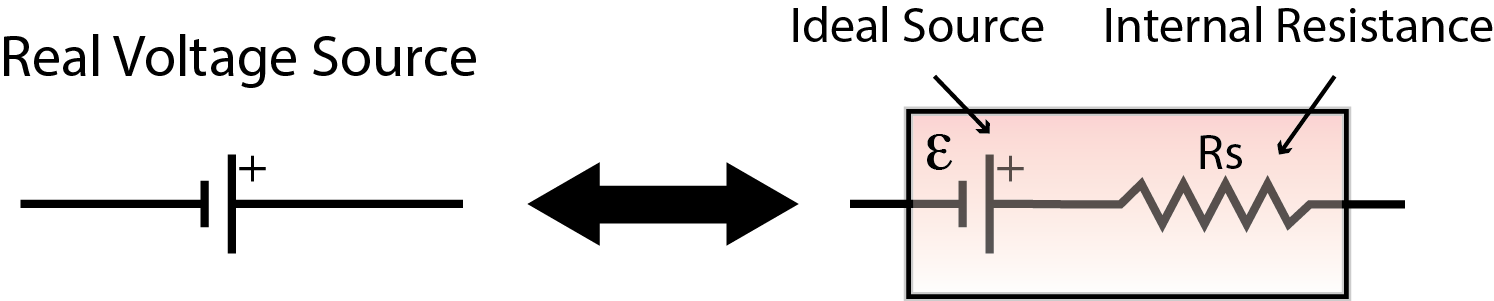
\includegraphics{real_vs_ideal_voltage}
\end{marginfigure}

In reality, the battery itself will have some internal ``source'' resistance $R_s$ which limits the current. We can thus model a real voltage source as a series combination of an ideal voltage source and an internal resistance, held inside a box that we can not open figure \ref{fig:real_vs_ideal_voltage}.



\begin{myexample}[label = ex:popquiz_intresistance]{Internal resistance of a battery}
A $9~V$ battery has an internal resistance of $1.5~\Omega$. What is the maximum current which the battery can provide? What is the power dissipated internally by the battery?

\Solution
From our work with ideal sources, Ohm's law tells us that:

$$
I_{max} = \frac{V_\text{ideal}}{R_s} = \frac{9~\text{V}}{1.5~\Omega} = 6~\text{A}
$$

\noindent This is an absurd amount of current. Before something very bad happens to the battery, it is dissipating an internal Joule heating of

$$
P = I^2_\text{max}R_s = I_\text{max}V\text{ideal} = 6~\text{A}\times9~\text{V} = 54~\text{W}
$$
\end{myexample}

\noindent  \textcolor{red}{\textbf{WARNING}}: This is why you never short-out a battery\footnote{i.e. why you never connect the terminals directly with a wire.}. The very high resultant current is now being dissipated by the internal resistance $R_s$ resulting in a lot of heat. This can cause a battery to explode or catch fire (see youtube for fun videos of this).

\subsection{Electromotive Force (EMF)}
There are an number of terms you will come across in the lab when dealing with sources. Among these is electromotive force (EMF) often written as $\mathcal{E}$. EMF is formally defined as maximum work available per charge when moving from position $\textbf{r}_A$ to $\textbf{r}_B$ along a path $\Gamma$:

\begin{equation}\label{eq:def_emf}
\mathcal{E} \equiv -\int_\Gamma\textbf{E}(\textbf{r})d\textbf{l}
\end{equation}

This can be a confusing term for many reasons.
\begin{enumerate}
\item Despite its name, EMF is not a force! It has units of Volts - its usage as a force is merely historical residue from the development of electricity and magnetism. 
\item Although often the terms voltage and EMF are used interchangeably, there are not the same fundamentally.\footnote{\textbf{Highbrow note on emf:} The real difference between EMF and voltage comes about in electro\textit{dynamics} and only outside the good-circuit model:

\begin{align*}
\mathcal{E} &\equiv -\int_a^b\mathbf{E}\cdot d\mathbf{l} \\ &= -\int_a^b\left(\nabla\phi - \frac{d}{dt}\mathbf{A}\right)\cdot d\mathbf{l} \\
&= -\Delta V + \frac{d}{dt}\int_a^b\mathbf{A}\cdot d\mathbf{l} 
\end{align*}

\noindent where $\phi$ and $\mathbf{A}$ are the electrodynamic scalar and vector potentials respectively. 


\noindent $\mathcal{E}$ and voltage are thus equivalent as long as $\frac{d}{dt}\int_a^b\mathbf{A}\cdot d\mathbf{l}  = 0$.} $\mathcal{E}$ is the work per unit charge and voltage is the difference in electric potential. However, in the regime relevant to electronics, they are practcally the same (see margin note).
\item EMF is sometimes used as a noun (i.e. the voltage) and sometimes used as a verb (the thing that causes the voltage.)
\end{enumerate}

We will use the convention that an EMF is a noun. In a battery $\mathcal{E}$ is equal to the amount of voltage that would be measured if precisely 0~amps of current were flowing. As soon as current begins to flow, the measured voltage drops, due to Ohm's law for the current through the internal resistance. A real source can be thus seen as a pure internal EMF with a resistor connected in series.


\section{Power Delivered to Load: Impedance Matching}
Suppose we want to power a device - a heater, light-bulb, or whatever with a real voltage source. Let our source have an ideal voltage $\mathcal{E}$ and output impedance $R_s$ and suppose we want to transfer as much power as possible to the load. The circuit, drawn in figure \label{fig:loadresistor}, introduces an interesting compromise: If we make the load resistance too large, hardly any current will be drawn in the circuit and the power delivered to the load $P = I^2R$ will be vanishingly small. On the other hand if we make $R_\text{load}$ too small, the current will be limited by $R_s$ and the power will again tend to 0 on account of $R_\text{load}\rightarrow 0$.

\begin{marginfigure}
\caption{Power delivered to a load in an non-ideal circuit.}
\label{fig:loadresistor}
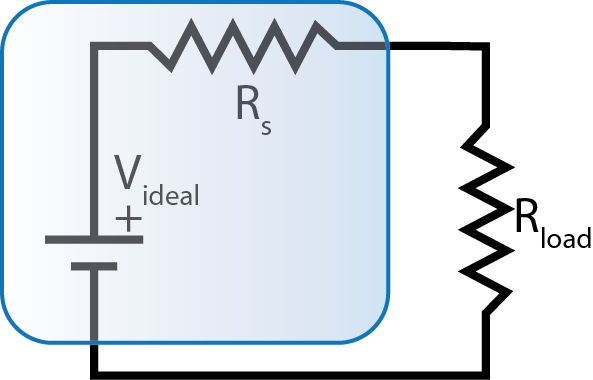
\includegraphics{loadresistor}
\end{marginfigure}

Since the power tends to zero as $R_\text{load}\rightarrow 0$ and $R_\text{load}\rightarrow \infty$, there must be a maximum somewhere. We can obtain this maximum by the standard tools of calculus and by noting that the circuit in figure \label{fig:loadresistor} is just a voltage divider with $V_\text{load} = V_\text{ideal}\times R_\text{load}/(R_s+R_\text{load})$. We then have:

\begin{equation}\label{eq:maxpow1}
P_\text{load} = \frac{V_\text{load}^2}{R_\text{load}} = \frac{R_\text{load}}{\left(R_\text{load}+R_s\right)^2}V_\text{load}^2
\end{equation}

\noindent Denoting $R_\text{load} \equiv r$ for brevity, we can take the derivative and set to 0:

$$
\frac{d P_\text{load}}{dr}  =  \frac{\left(R_s+r\right)^2 - 2r\left(R_s+r\right)}{\left(R_s+r\right)^4}
$$

\noindent or,

$$
\left(R_s+r\right)^2 - 2r\left(R_s+r\right) = 0
$$
\noindent which is satisfied when

\begin{equation}\label{eq:maxpow}
r = R_\text{load} = R_s
\end{equation}

Thus the maximum power is delivered when the input resistance of the load matches the output resistance of the source. This is a case of as important concept known as impedance matching. This is especially relevant for high frequency signals which are patched through various lab instruments for which all devices must be matched or have special impedance matching devices at the input.

% XSSSSSXSXSXSXSXSXSXSXSXXSXS

\section{Th\'evenin's Theorem}
In the above example, consider the situation from the point of view of the load resistor: all it ``knows'' is that there is some electric field produced by any combination of sources and resistors. It has no idea whether there is a single battery, 5 batteries, or a magician with a wand creating the field, it just ``feels'' a potential difference. This philosophy of looking at the circuit in terms of the loads, not the sources leads to a powerful technique for analyzing circuits known as \textit{Th\'evenin's theorem}:

\noindent\textbf{Th\'evenin's Theorem:} \textit{Any network of voltage sources, resistors, and current sources can be replaced by a single equivalent voltage source $V_\text{th}$, in series with a single equivalent resistance $R_\text{th}$.}

\begin{figure}[h]
\caption{Any linear circuit can be viewed as a ideal voltage source in series with a resistor.}
\label{fig:thevenin}
\begin{center}
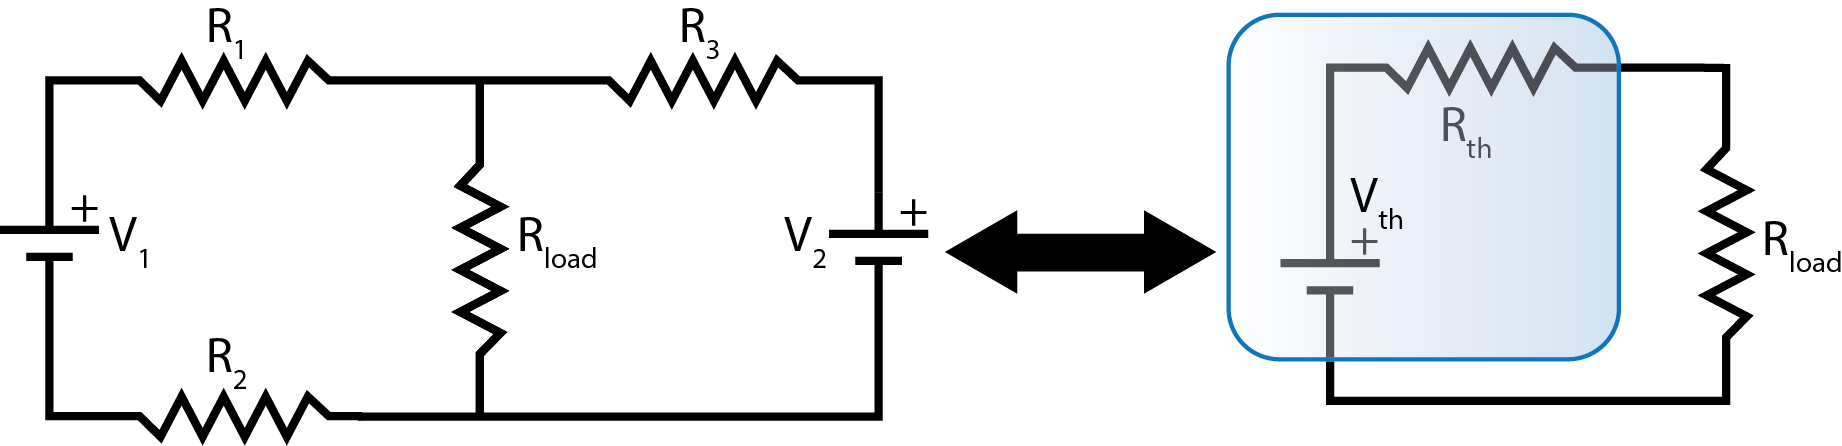
\includegraphics[width=\textwidth]{thevenin.png}
\end{center}
\end{figure}

With reference to figure \ref{fig:thevenin}, Th\'evenin's theorem states that the complicated network shown on the left in figure \ref{fig:thevenin} can be replaced with the simple circuit on the right. Notice that the figure on the right is merely a voltage divider which we have already studied. This provides a convenient method for determining the effect of loading on a circuit: we can simply obtain $V_\text{th}$ and $R_\text{th}$ and apply the standard voltage divider equation: $V_\text{load} = V_\text{th}\times R_\text{load}/(R_\text{th}+R_\text{load})$. We begin to see a recurring theme in this course: most of electronics can be reduced to a voltage divider. But how do we get $V_\text{th}$ and $R_\text{th}$? There are two approaches:

\begin{myexample}[label = ex:det_thev_exp]{Determining $V_\text{th}$ and $R_\text{th}$ Experimentally}

{\centering
     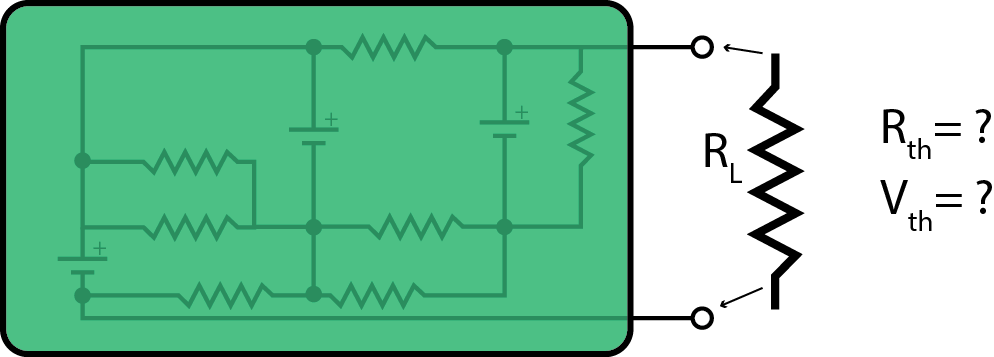
\includegraphics{thvn_ex_1.png}
      \par
}

Suppose that we have a complicated circuit that we want to drive a load with and we want to know the internal voltage and output impedance. How might we do this?

\noindent Note that Thevenin's theroem states that we can always reduce the circuit to a voltage divider driving a load. Suppose that when we plug a 25$~\Omega$ load resistor in the circuit, we measure a 2~V drop and when we use a 400$~\Omega$ load, we find a voltage drop of 8~V. This gives us two equations in 2 unknowns and is sufficient to solve the system completely. Using:
\begin{eqnarray*}
V_L & = &  \frac{R_L}{R_\text{th} + R_L}V_\text{th}\text{             ... or} \\
V_\text{th} R_L &=& \left(R_\text{th} + R_L\right)V_\text{th}
\end{eqnarray*}
\noindent we have:
\begin{eqnarray*}
25V_\text{th} &=& 2R_\text{th} + 50 \\
400V_\text{th} &=& 8R_\text{th} + 3200
\end{eqnarray*}

\noindent Subtracting 4 times the first equation by the second gives $300V_\text{th} = 3000R_\text{th}$, or $V_\text{th} = 10V$. Inserting this into either equation yields $R_\text{th}$:


\begin{eqnarray*}
V_\text{th} & = & 10V \\
R_\text{th} & = & 100\Omega
\end{eqnarray*}

\noindent Note that this result is independent of the load resistance. Having determined the equivalent circuit, we know how it will behave for all loads.
\end{myexample}

We can also determine the Thevenin equivalent circuit theoretically. As it turns out there is a cookbook recipe for doing so:

\textbf{Th\'evenin Algorithm}

\noindent To calculate the equivalent network resistance across two nodes:

\noindent\textbf{Step 1} Remove any load element(s) between the two nodes and calculate the resultant ``open circuit'' voltage. This is $V_\text{th}$.

\noindent\textbf{Step 2} Short circuit all voltage sources (i.e. replace them with a wire) and find the equivalent resistance between the output nodes. This is $R_\text{th}$.



\begin{myexample}[label = ex:thev_theo]{Determining $V_\text{th}$ and $R_\text{th}$}
We mentioned that we can use a voltage divider to provide a voltage source of desired voltage. How does circuit loading affect the voltage divider circuit?

\noindent We can use the Thevenin approach to determine the output resistance and effective voltage of our voltage divider. Figure~\ref{fig:thvn_ex_2}a shows our circuit with an arbitrary load $R_L$ connencted. We proceed to use the Thevenin algorithm:

\noindent \textbf{Step 1}: Remove the load and determine the equivalent voltage (figure ~\ref{fig:thvn_ex_2}b). We see that the voltage is just that of the original, ideal voltage that we already have studied:

$$
V_\text{th} = \frac{R_2}{R_1+R_2}V_0
$$

\noindent \textbf{Step 2}: Short circuit the sources and determine the equivalent resistance (figure ~\ref{fig:thvn_ex_2}c). We see that the equivalent resistance is merely a parallel combination of $R_1$ and $R_2$.

$$
R_\text{th} = \frac{R_1R_2}{R_1+R_2}
$$

\noindent The resultant circuit is just a new voltage divider with:

$$
V_\text{out} = \frac{R_L}{R_\text{th}+R_L}V_\text{th}
$$

Noting that an ideal source in this case satisfies $V_\text{out} = V_\text{th}$. A ``good'' voltage divider will have $R_\text{th} \ll R_L$. One should not make it arbitrarily low however, since in that case a large amount of current will have to flow through $R_2$ as compared to the load and will be inefficient.
\end{myexample}

\begin{figure}[h]
\caption{Using Thevenin's theorem to study a real-world voltage divider.}
\label{fig:thvn_ex_2}
\begin{center}
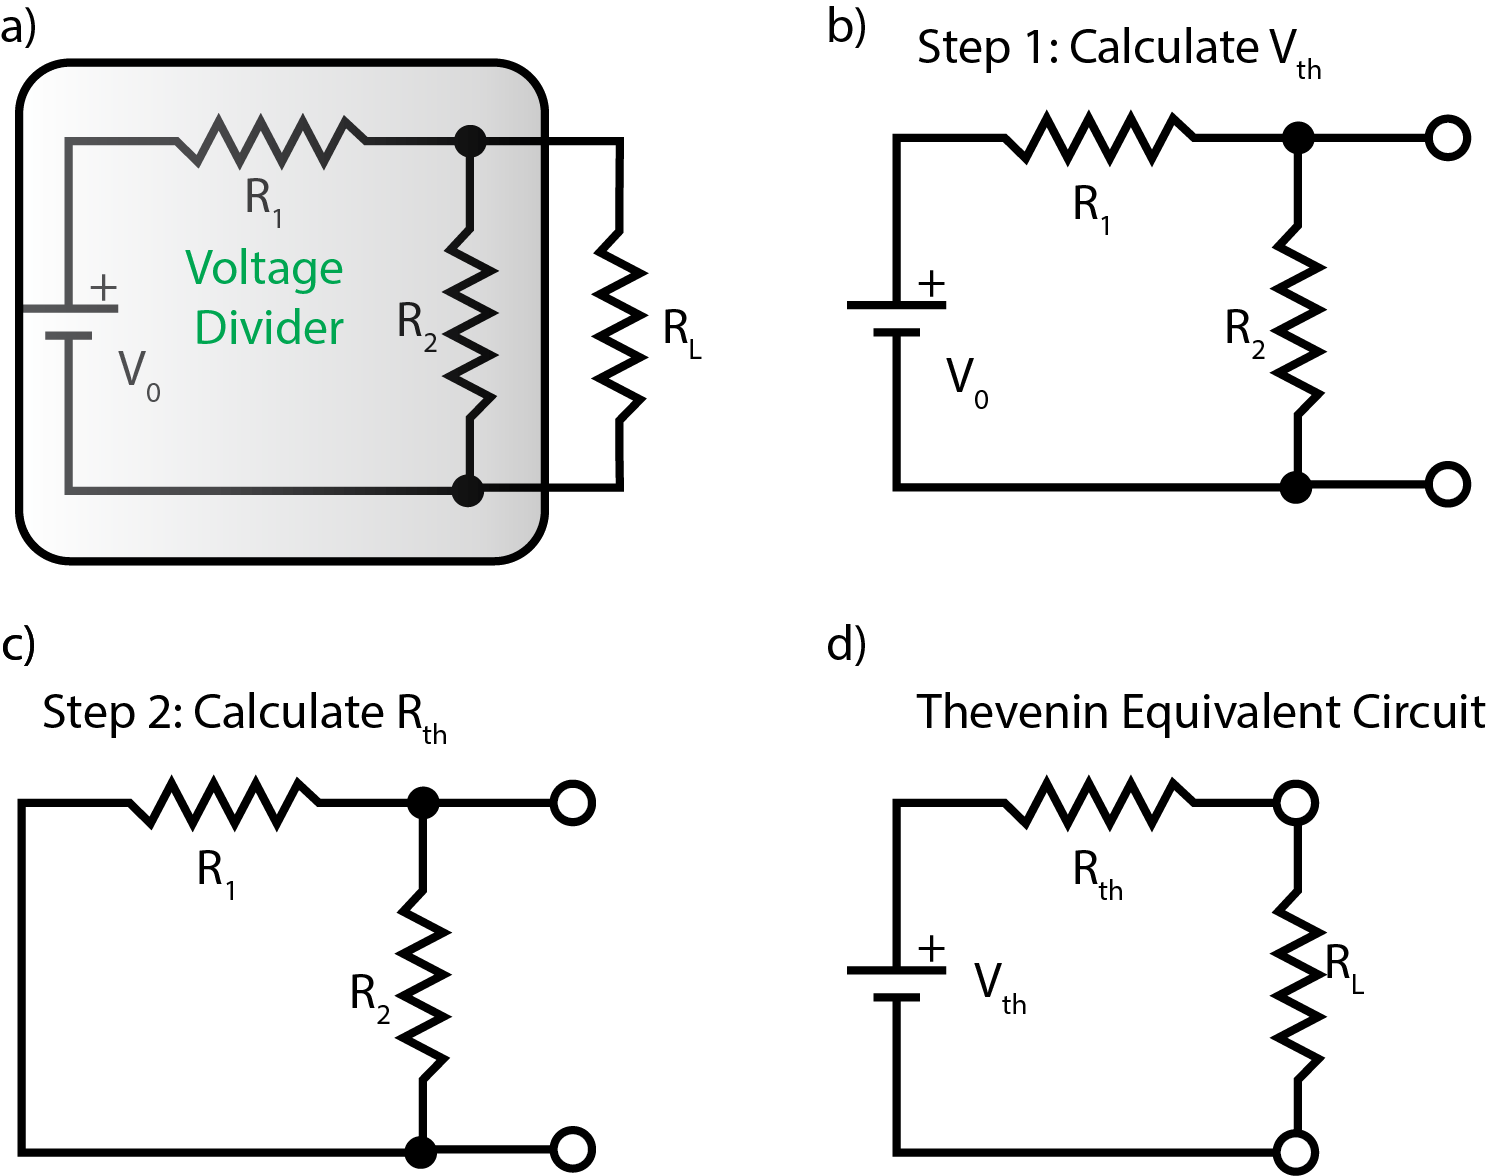
\includegraphics[width=\textwidth]{thvn_ex_2.png}
\end{center}
\end{figure}


\chapter{Introduction to AC Circuits}
\section{AC/DC}

So far, we have dealt with time independent voltages, i.e. when we analyze a circuit with a 9V battery and a 1~k$\Omega$  resistor, we say that the current is 9~mA (forever). Often in experimental settings, this is not the case, for example a particle detector may give a short pulse whenever a photon hits its surface. Even more commonly the voltage coming out of a wall outlet is a periodic (sine) waveform repeating itself 60 times per second\footnote{... in North America.} (figure \ref{fig:ACexamples}).

By convention signals (currents or voltages) which are constant in time are called Direct Current or \textbf{DC}, and signals which vary in time are called Alternating Current \textbf{AC}. AC signals can be divided up into periodic and non-periodic. Periodic signals precisely repeat themselves after some time.

Why is this an issue? As it turns out, voltages and currents have a characteristic settling time leading to time delays which we have neglected in our analysis of DC circuits. The laws of electromagnetism requires an interplay of electric and magnetic fields which arises whenever the constituent fields change over time - a changing voltage or electric field necessitates will create a magnetic field and a change in this magnetic field creates new electric fields. Our goal is to encapsulate the complicated electrodynamics and resultant time delays into a simple formalism where we don't worry about the fundamental fields in the same way we did with DC circuits. Fortunately, a simple formalism exists and is only a small incremental step from what has been developed thus far.

\begin{figure}[h]
\caption{DC Signals are constant in time, AC signals are not. AC signals can be periodic (right), or not (center).}
\label{fig:ACexamples}
\begin{center}
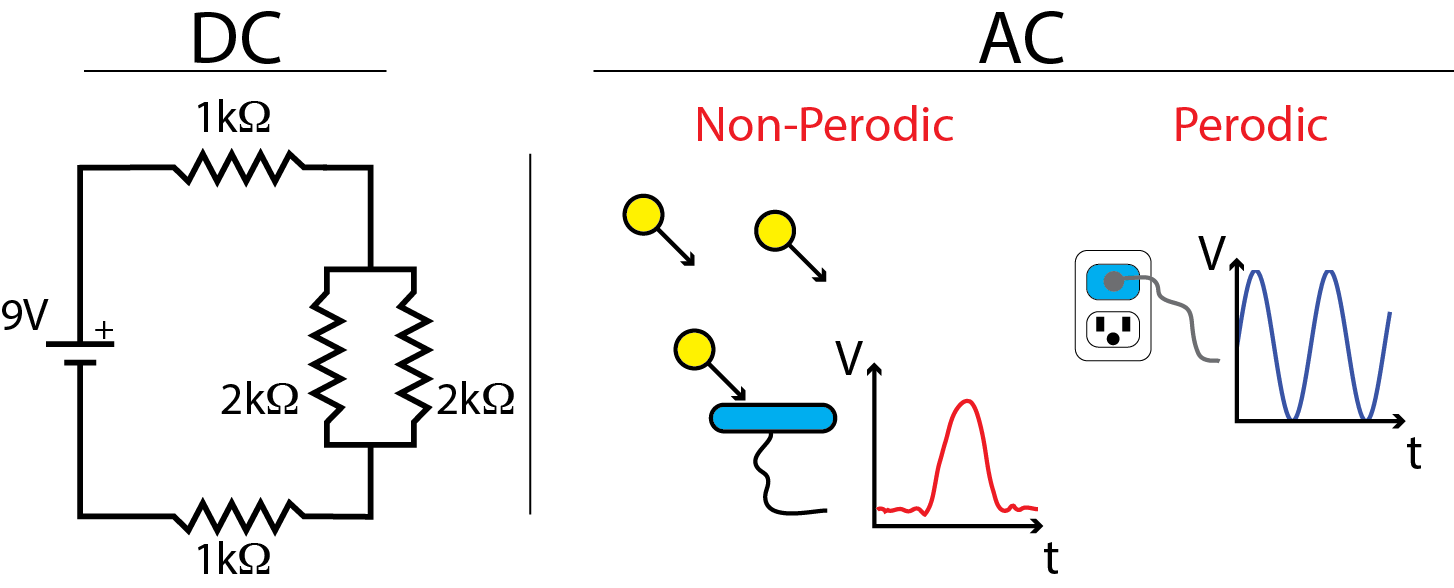
\includegraphics[width=\textwidth]{ACexamples}
\end{center}
\end{figure}

\section{Sinusoidal waveforms}
The workhorse of AC electronics is the sine-wave. For reasons that will become clear soon, when you understand the way a sinusoidal voltage behaves in a circuit, you understand just about everything in the circuit. Fir this reason we will spend some time becoming familiar with different ways of representing sine waves and its related quantities. This will lead us down a rabbit hole of using complex numbers to represent real things such as voltage which will seem crazy at first but will be made worth while. 

\begin{marginfigure}
\caption{Sine waves. The left shows the time-based quantities, the right shows the voltage-based quantities}
\label{fig:sinewaves}
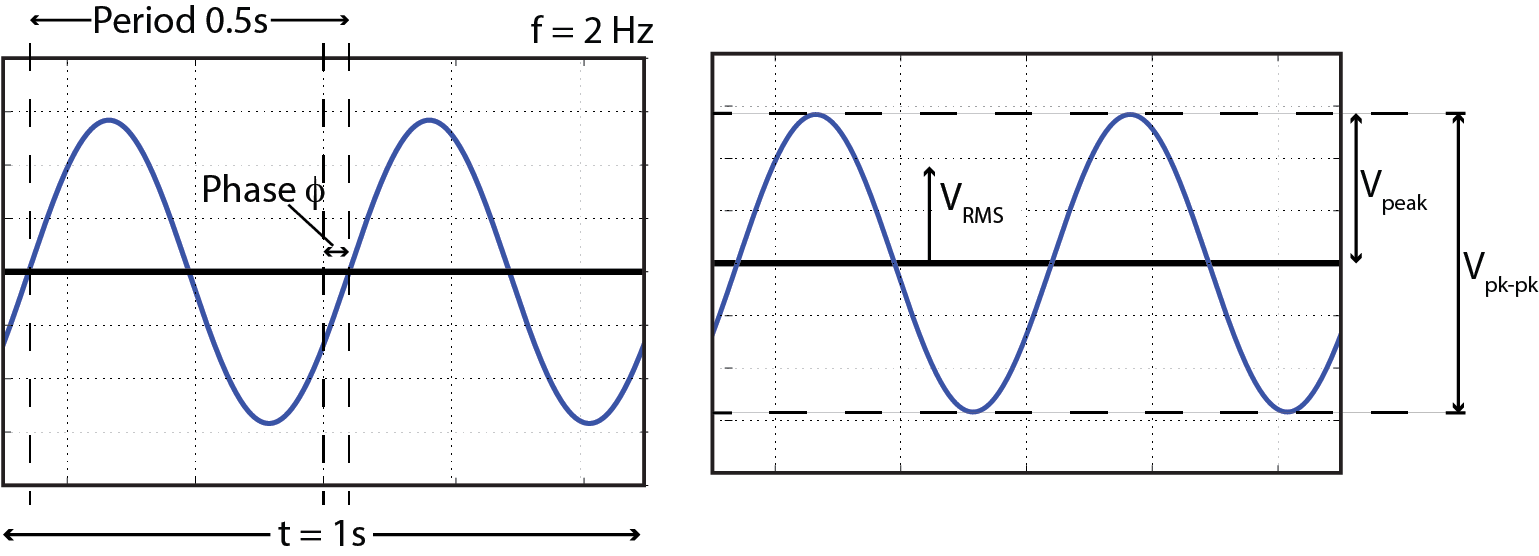
\includegraphics[width=\textwidth]{sinewavez}
\end{marginfigure}


Figure \ref{fig:sinewaves} shows a sinusoidal voltage given by the equation:

\begin{equation}\label{eq:sinus}
v(t) = A\sin(2\pi f t + \phi) = A\sin(\omega t +\phi)
\end{equation}

There are a few fundamental quantities immediately observable from this plot:

\subsection{Period and Frequency}
The recall that any periodic signal is one that precisely repeats after a fixed time $T$. The \textbf{period} is defined as this time. The \textbf{frequency} $f$ is number of times per second that the pattern repeats and is thus the reciprocal of the period:

\begin{equation}\label{def:frequency}
f \equiv\frac{1}{T}
\end{equation}

One often uses the \textbf{angular frequency} $\omega$ in place of $f$ since a sine or cos wave repeats itself at every multiple of $\pi$. Note $\omega$ is merely a scaled $f$ and contains no new information:

\begin{equation}\label{def:angfreq}
\omega \equiv 2\pi f = \frac{2\pi}{T}
\end{equation}

\subsection{Phase}
The quantity $\phi$ is known as the phase shift of the signal. Note that if $\phi=0$ the signal goes through zero at $t=0$. If however $\phi\ne0$ the signal is merely shifted in time. To see this note that:

\begin{equation}\label{eq:phase_shift}
\sin\left[\omega t + \phi\right] = \sin\left[\omega\left(t  + \frac{\phi}{\omega}\right)\right] = \sin\left[\omega\left(t  + \Delta t\right)\right]
\end{equation}

\noindent ... with 

\begin{equation}\label{eq:phase_shift2}
\phi = \omega\Delta t
\end{equation}

We thus see that a phase shift is equivalent to a time delay. This s important since we will now be able to treat temporal delays in our AC circuits as phase shifts of sinusoidal signals.

\subsection{Amplitude and Peak to Peak}
The function in figure \ref{eq:sinus} is bounded between $-A$ and $A$. The quantity $A$ is known as the \textbf{Amplitude} of the signal. Recalling that only differences in potential are meaningful, one often uses the \textit{peak-to-peak} voltage:

\begin{equation}\label{def:Vpp}
V_{pp}\equiv V_\text{max} - V_\text{min}
\end{equation}

\subsection{RMS and Peak to Peak Voltage}
Recall that the power delivered to a resistor by a DC voltage is given by $V^2/R$ (eq. \ref{eq:joule_ohm}). Since the voltage in an AC signal is time dependant, so is the power delivered at a given time. However, given the definition of power as the energy delivered per unit time $P\equiv dE/dt$, one would like to know the average power delivered to a resistor over many cycles. For example, a load plugged into the wall voltage goes through 60 cycles per second - so how much energy is deposited over that second? For this we can use the average power per cycle. 

Note that the average voltage over one (or many) cycles is zero, but owing to the square of the voltage in eq. eq. \ref{eq:joule_ohm}, the power delivered is independent of the sign. Clearly then the power is non-zero and positive. In fact it is given by $\bar{V^2}/R$. Comparing this to $V^2/R$, we see that this is equivalent to a DC voltage of a given voltage known as the RMS or \textit{root-mean-square} voltage defined as the squared voltage, averaged over one complete cycle:

\begin{equation}\label{def:Vrms}
V_\text{RMS}\equiv \sqrt{\langle v^2(t)\rangle_T} = \sqrt{\frac{\int_0^Tv^2(t)dt}{T}}
\end{equation}

\noindent RMS current is defined in precisely the same way.

\begin{myexample}[label = ex:rms_sine]{RMS of a Sine wave.}
For a sine wave $v(t) = A\sin(\omega t)$, compute the rms voltage.
\Solution
By definition, we have:
$$
V_\text{RMS} = \sqrt{\frac{1}{T}\int_0^TA^2\sin^2(\omega t)dt} = A\sqrt{\int_0^T\sin(2\pi\frac{t}{T}) \frac{dt}{T}}
$$

\noindent Letting $\tau\equiv t/T$, we have:
\begin{align*}
V_\text{RMS} &= A\sqrt{\int_{\tau=0}^1\sin^2 (2\pi \tau) d\tau} \\
&=  A\sqrt{\int_{\tau=0}^1\left[\frac{1}{2}-\frac{1}{2}\cos(4\pi\tau)\right]d\tau} \\
&= \frac{A}{\sqrt{2}} \\
&\approx 0.707A
\end{align*}
\end{myexample}

\subsection{AC and DC Components of signals}
So far we have analyzed sine waves with zero-mean but this is generally not the case. Figure \ref{fig:ACcomp} shows a sine wave that has a 1~V offset. We call the mean value the \textit{DC component} of the signal. The \textit{AC component} of the signal is the remaining signal after subtracting the mean. The signal is the sum of its DC and AC components. 

\begin{marginfigure}
\caption{A signal can be split into AC and DC components.}
\label{fig:ACcomp}
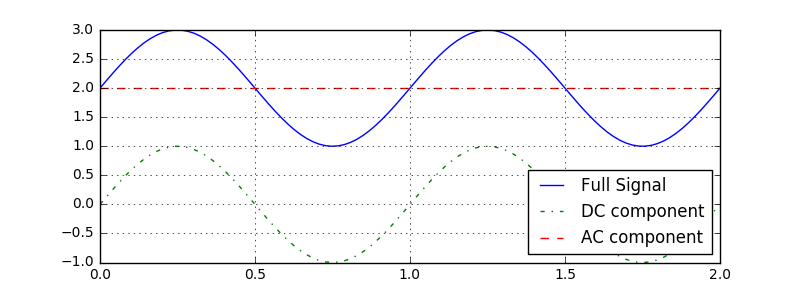
\includegraphics[width=\textwidth]{ACcomp}
\end{marginfigure}

In experimental physics we are interested in a small perturbation of a large net signal. For example we may want to observe a periodic emission of single photons from an atomic vapour or the dip in light due the transient of an exo-planet in front of a star. In these cases we are strictly interested in the AC signal and the DC signal is a nuisance. Later in the course and in the labs, we will construct circuit elements known as ``filters'' which isolate the AC- and DC- components of a given signal.

%%% ========================================================================
\section{Complex Numbers}

As it turns out, the analysis of AC signals is much, much (much) easier using the machinery of complex numbers. You may or may not have come across complex math before in your studies, but fortunately one does not need to be an expert on complex analysis to benefit from its simplifications. This is one instance where you will have to have a little faith that this strange way of representing signals will pay itself back many-fold in simplicity in in the duration of the course. It is not clear \textit{a priori}, why you would do things this way and if you were starting from scratch with no foresight, you probably wouldn't. It has merely been discovered after the fact that using a complex number representation makes understanding circuits much simpler and avoids pages of tedious mathematics. 

In high school, you all learned how to solve the quadratic equation:

$$
ax^2 + bx + c = 0
$$

\noindent having solution:

$$
x = -\frac{b}{2a} \pm \frac{b^2-4ac}{2a}
$$

If the so called ``discriminant'' $b^2 - 4ac$ was negative, we were told that there was no solution since the square root of an imaginary number is nonsense. However to a mathematician named Euler who lived a few centuries ago, this cop-out was unacceptable. He found that if we simply denote the square root of $-1$ a symbol\footnote{Commonly in physics, the symbol is $i$ for ``imaginary'' but since in electronics, $i$ is spoken for by current, engineers tend to find the closest shape to an $i$ - a lower case $j$ in stead.} $j$, a whole new world of possibilities opened up. Now the quadratic equation didn't have 0, 1, or 2 roots, but always 2. Further more - every $n^{\text{th}}$ order polynomial had precisely $n$ roots. A result known as the ``fundamental theorem of algebra''. This all works provided that we agree that $j^2 = -1$. 

\begin{equation}\label{def_imagnum}
j \equiv \sqrt{-1}
\end{equation}

\noindent For example, the equation $x^2 + 4 = 0$ can now be solved via:

\begin{align*}
x^2 &= -4 \\
x &= \pm \sqrt{-4}  \\
&= \pm \sqrt{4}\sqrt{-1} \\
&= \pm2j
\end{align*}

\subsection{Complex arithmetic}
The number in the above example is known as a pure-imaginary number, that is a real number times $j$. In general however, we can have a mix of real and imaginary number, forming what is known as a \textit{complex number}:

\begin{equation}\label{def:cpxnum}
z = a + ib
\end{equation}

\noindent The quantities $a$ and $b$ are called the \textit{real} and \textit{imaginary} parts of $z$.

Complex numbers can be added subtracted, multiplied and divided as you could any other number. The trick, as laid out in the following example, is to treat $j$ as a variable, but replace $j^2$ with $-1$.

\begin{myexample}[label = ex:its_complicated]{Complex Artithmetic.}
Let $z_1 = 2+3j$ and $z_2 = 1-4j$. Compute (a) $z_3 = z_1 + z_2$ and (b) $z4 = z_1\times z_2$.

(a) \begin{align*}
z_3  &= z_1+z_2 \\
& = \left(2+3j\right) + \left(1-4j\right) \\
&=  \left(2+1\right) + (3-4)j \\
&= 3 -1j
\end{align*}

(b)\begin{align*}
z_4  &= z_1\times z_2 \\
& = \left(2+3j\right) \left(1-4j\right) \\
&=  2 - 8j + 3j -12j^2 \\
&= 2 - 5j -(-12) \\
&= 14-5j
\end{align*}
\end{myexample}

\subsection{Graphical Representation of Complex Numbers}
A useful way of representing complex numbers is to place them on a two dimensional graph with the horizontal axis representing the real part and the vertical axis representing the imaginary part of the number (see figure \ref{fig:argand}a). Plotting numbers on this plane, formally known as the ``Argand'' plane provides a useful visualization addition and subtraction akin to vector additions, figure \ref{fig:argand}b displays the addition of $z_1+z_2$ from the previous example, graphically. 

\begin{marginfigure}
\caption{(a) The Argand plane represents the complex number $a+bj$ graphically. (b) The graphical representation provides a useful visual guide for addition. Here $z_3 = z_1 + z_2$ is displayed with $z_1 = 2+3j$ and $z_2 = 1-4j$}
\label{fig:argand}
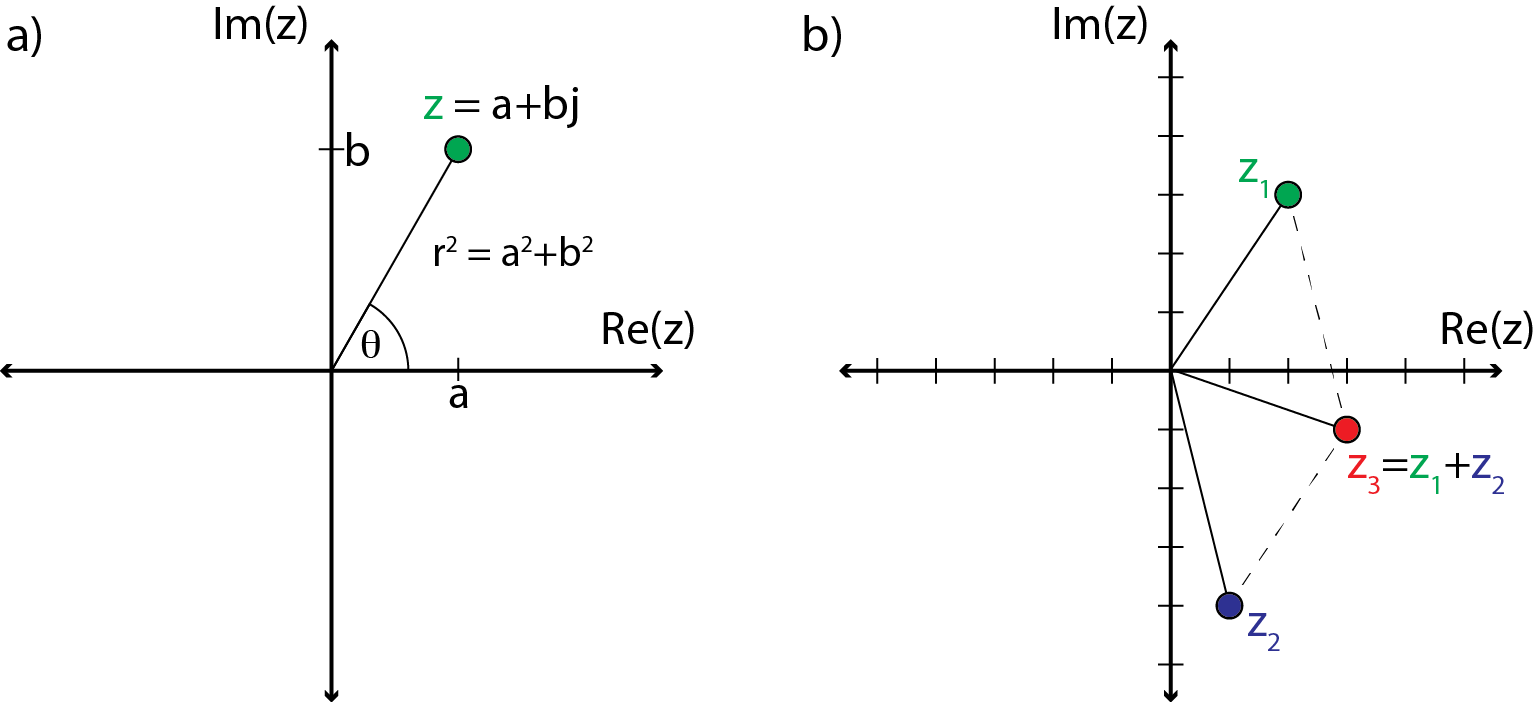
\includegraphics[width=\textwidth]{argand.png}
\end{marginfigure}

The representation of complex numbers in the Argand plane suggests a new representation of the complex number, akin to polar coordinates you are familiar with from ordinary algebra. Specifically we can write $z$ as:

\begin{equation}\label{eq:polar_cpx}
z = a+jb = \cos\theta + j\sin\theta
\end{equation}


\subsection{Euler's magical formula}
Something truly remarkable occurs when you write out the Taylor series expansion of equation \ref{eq:polar_cpx}. We find that the sum of a cosine and $j$ times a cosine s somehow equal to the mathematical constant $e$ raise to an imaginary power:

\begin{equation}\label{eq:eulers}
e^{j\theta} = \cos\theta + j\sin\theta
\end{equation}

This remarkable fact will be worth it's weight in gold both in this class and in much of the physics to come during your education. 


\textbf{Theorem:} For real numbers $r$ and $\theta$

$$
e^{j\theta} = \cos\theta + j\sin\theta
$$

This theorem may be proven by comparing Taylor series\footnote
{
\textbf{Proof:} Recall the following Taylor series:
\begin{align*}
\cos\theta  &= \sum_{k=0}^\infty\frac{\left(-1\right)^k}{\left(2k\right)!}\theta^{2k} = 1 - \frac{\theta^2}{2} + \frac{\theta^4}{4!} + \cdots \\
\sin\theta  &= \sum_{k=0}^\infty\frac{\left(-1\right)^k}{\left(2k+1\right)!}\theta^{2k+1} = \theta + \frac{\theta^3}{3!} - \frac{\theta^5}{5!} + \cdots \\
\exp{\theta} &= \sum_{k=0}^\infty \frac{\theta^k}{k!} = 1 + \theta + \frac{\theta^2}{2} + \frac{\theta^3}{3!} + \cdots
\end{align*}

Thus:
\begin{align*}
\exp^{j\theta} &= 1 + j\theta + \frac{\left(j\theta\right)^2}{2!} +  \frac{\left(j\theta\right)^3}{3!} +  \frac{\left(j\theta\right)^4}{4!} + \cdots \\
&= 1 + j\theta - \frac{\left(\theta\right)^2}{2!} -  j\frac{\left(\theta\right)^3}{3!} + \frac{\left(\theta\right)^4}{4!} + \cdots \\
&= \left[1-\frac{\theta^2}{2!}+\frac{\theta^4}{4!} +\cdots\right] + j\left[\theta -\frac{\theta^3}{3!} + \frac{\theta^6}{6!} + \cdots\right] \\
&= \cos\theta + j\sin\theta 
\end{align*}
}

\noindent Eulers Formula allows us to choose between ``Cartesian'' or ``polar'' representations of complex numbers. You can go from one to the other easily:

\noindent\textbf{polar $\rightarrow$ cartesian}: Starting with $z = re^{j\theta}$, we directly write $z = r\cos\theta + rj\sin\theta$ and so $z = a + jb$ with $a = r\cos\theta$ and $b = r\sin\theta$.

\noindent\textbf{cartesian $\rightarrow$ polar}: Starting with $z = a+ib$, we have the magnitude $r = \sqrt{a^2+b^2}$. The angle we get from the Argand diagram: $b/a = \tan\theta$, or $\theta = \arctan\frac{b}{a}$. We then use these values and write $z = re^{j\theta}$.

\noindent While both representations are equivalent, one may be more convenient that the other for a particular operation. For example, division and multiplication requires some algebra in cartesian coordinates but is trivial in polar:

$$
r_1e^{j\theta_1}\times r_2e^{j\theta_2} = r_1r_2e^{j\left(\theta_1+\theta_2\right)}
$$

\noindent Addition or subtraction on the other hand is handled more directly in Cartesian form.

\subsection{Complex Conjugation, Magnitude and phase}
Recall that the magnitude $r$ of a 2 dimensional vector $(a,b)$ is given geometrically by $r^2 = a^2 + b^2$. We can likewise speak of the magnitude of a complex number. Consider an arbitrary complex number $z = a + jb$. The square of this number is $z^2 = a^2 - b^2 +2jab$ which is clearly not what we are after. Consider however the quantity $\bar{z} \equiv a-jb$. Then:

$$
 z\bar{z} = \left(a+jb\right)\left(a-jb\right) = a^2 -jab +jab -j^2b^2 = a^2 + b^2
$$

The quantity $\bar{z}$ is known as the \textit{complex conjugate} and is of paramount importance when working with complex numbers. In polar coordinates the conjugate of $z=re^{j\theta}$ is $\bar z = re^{-j\theta}$. In general, the conjugate is arrived at by interchanging $j\leftrightarrow-j$.

\noindent The \textit{magnitude} $r$ of a complex number is given by:

\begin{equation}\label{def:cpx_mag}
z = a+jb \rightarrow\bar{z} = a -jb
\end{equation}

\noindent Another common quantity is the phase or \textit{argument} of a complex number. This is simply the angle that the complex number makes in the polar representation:
\begin{equation}\label{def:cpx_phs}
\arg z \equiv \arctan{\frac{\Im m [z]}{\Re e [z]}}
\end{equation}

\subsection{Complex Fractions}

There are a huge assortment of operations one can perform on complex numbers and we will not go over many detailed examples. However, a very common situation relevant to this course material is to take a complex fraction and put it into either Cartesian or polar form:

$$
z = \frac{z_1}{z_2} = \frac{a_1+jb_1}{a_2+jb_2} \rightarrow a_0 +jb_0 \rightarrow re^{j\theta} 
$$

The standard method of doing this is to multiply top and bottom by the complex conjugate of the denominator. Then you have a complex number in the numerator divided by a real number which is trivial. An example is worth a thousand words:

\begin{myexample}[label = ex:its_complicateder]{Complex division.}
Let $z_1 = 1 + 3j$ and $z_2 = 2 + j$. Compute 
$$
\frac{z_1}{z_2} = \frac{1 + 3j}{2 + j}
$$
\noindent... (a) in cartesian form and (b) in polar form

(a) \begin{align*}
\frac{z_1}{z_2}  &= \frac{z_1\bar{z_2}}{z_2\bar{z_2}} \\
& = \frac{\left(1+3j\right)\left(2-j\right)}{\left(2+j\right)\left(2-j\right)} \\
&=  \frac{2+3 + 6j-j}{5} \\
&= \frac{5}{5} + \frac{5}{5}j \\
z &= 1+j
\end{align*}
\\
(b)\begin{align*}
r &= \sqrt{(1+j)(1-j)} = \sqrt{2} \\
\theta &= \arctan{1/1} = \pi/4 \\
z &= \sqrt{2}e^{j\pi/4}
\end{align*}
\end{myexample}

\subsection{Representing Voltages with Complex Numbers}
Now that we have gone through all of the trouble of learning complex numbers it's time et something useful back. Euler's formula suggests that there is a correspondence between a number $re^{j\omega t}$ and $A\sin\omega t$. Indeed there is and there is a trick to do this which is used very often in the physics of oscillating systems:

\begin{enumerate}
\item We represent the oscillating voltage as a complex exponential: $A\cos\omega t \rightarrow Ae^{j\omega t + \phi}$
\item We perform all our mathematical operation on the signal $Ae^{j\omega t + \phi}\rightarrow A'e^{j\omega t +\phi'}$
\item We get the mesaurable signal by \textbf{taking the real part} of the number: $A'e^{j\omega t +\phi'} \rightarrow A'\cos(j\omega t +\phi')$
\end{enumerate}

Note that a complex number has 2 degrees of freedom - that is, a single complex number contains two independent pieces of information. This is crucial to their utility as it allows is to encapsulate both the magnitude and phase of a signal at once. Also note that we used $\cos$ in place of $\sin$. This was merely for convenience and has no bearing in the system - a cosine is just a sine with a particular phase (of $\pi/2$).

\section{The Digital Oscilloscope}
Recall that for our DC measurements of voltage, resistance and current, the DMM was our weapon of choice for measurements and analysis. For AC measurements, the corresponding tool is the Digital Oscilloscope.
The primary advantage of an oscilloscope over a DMM, is its ability of measure time dependent effects with a high degree of accuracy. 
Figure~\ref{fig:TDS2012C} displays the type of oscilloscope used in this lab - the Tektronix Model TDS 2012C Digital Oscilloscope. 
The y-axis displays voltage and the x-axis is time, giving us a dynamic “voltage vs. time” graph of the signal being measured. 
The time and voltage scales can be easily modified using the scale knobs. 

\subsection*{The Oscilloscope}
\begin{figure}[h]
\caption{TDS 2012C Digital Oscilloscope.}
\label{fig:TDS2012C}
\begin{center}
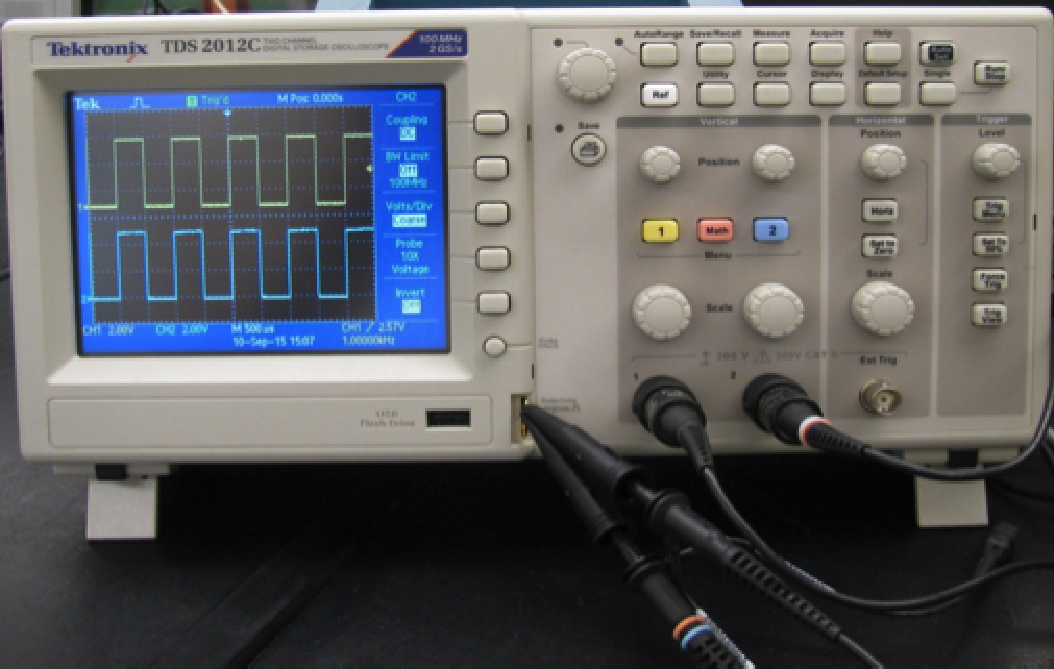
\includegraphics[width=\textwidth]{TDS_scope}
\end{center}
\end{figure}

You will make heavy use of the scope in virtually all remaining labs this course. Refer to the lab manual and the supplementary course information for further details on the operation and utility of the digital oscilloscope.

\section{Time Domain vs Frequency Domain: Fourier Analysis}\label{sec:fourier}
The importance of understanding the behaviour of sine waves in a system stems from a concept known as Fourier analysis. The essential concept behind Fourier analysis is that we can represent any signal as a sum of sine waves of a particular phase. There are really two sides to this coin. 

\textbf{One side}, which is very useful in finding solutions to differential equations is that a given periodic function $f(t)$ with period $T= 2\pi/\omega$ can write this be written as an infinite sum of sine and cosines having integer multiples frequencies of $\omega$:

$$
f(t) = \sum_{k=0}^\infty\left[a_k\cos k\omega t + b_k\sin k\omega t\right]
$$

\noindent Figure \ref{fig:FourierSeries} shows the first few terms in the Fourier series representing a triangle wave.

\begin{figure}[h]
\caption{The first 8 terms in the Fourier series approximation of a ``sawtooth'' wave.}
\label{fig:FourierSeries}
\begin{center}
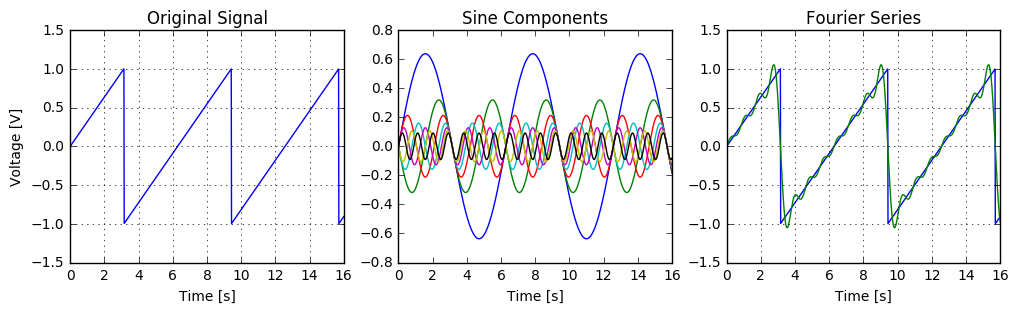
\includegraphics[width=13cm]{FourierSeries.png}
\end{center}
\end{figure}

\textbf{The other side}, which is more directly relevant to this course states that any continuous function in \textit{time} can be mapped on to a corresponding function in \textit{frequency} via a mathematical tool known as the \textit{Fourier Transform}:

\begin{equation}\label{def:fouriertransform}
F(\omega) = \frac{1}{2\pi}\int_{-\infty}^{\infty}e^{j\omega t}f(t)dt
\end{equation}

\noindent This introduces an entirely new way of looking at the world - we can either look at things happening in time, i.e. the \textit{Time Domain}, or by things happening in frequency, i.e. the \textit{Frequency Domain}. The Fourier transform acts as a gate between these two worlds. Figure \ref{fig:FourierExamples} shows a few examples of traces in the time and frequency domains.

Frequency Domain analysis asserts that once we understand how a circuit responds to a sine wave of an arbitrary frequency, we understand how any signal behaves. You will become familiar with Fourier techniques in the lab sections of this course.

\begin{figure}[h]
\caption{Time and frequency domain pictures of a sine wave, a square wave, and a small signal buried in noise.}
\label{fig:FourierExamples}
\begin{center}
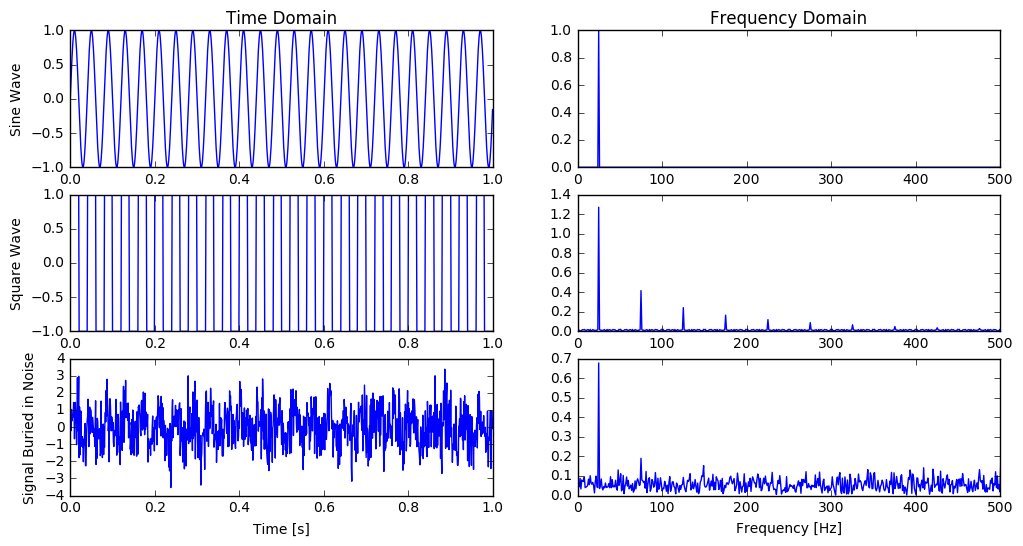
\includegraphics[width=\textwidth]{FourierExamples}
\end{center}
\end{figure}


%%% ========================================================================
\chapter{Reactive Circuits: Capacitors and Inductors}

\section{The Big Picture}

Our circuits thus far have been comprised of batteries and resistors. When we place an AC voltage across a resistor, we found that we could apply the same analysis as in our DC circuits, using the RMS value for the voltage. We did not have to give any information about the frequency of the signal. This is because in our good circuit model, the current in a pure resistance responds instantaneously to the voltage. We now move to circuit elements for which there is a finite time response to a time dependant voltage, causing a frequency dependant response to the signal. The two main devices we will study are the capacitor and the inductor. 

A hand wavy intuition of how these devices function stems from a simple fact about the nature of electromagnetic fields. The laws of electromagnetism are provide by fundamental laws known as Maxwell's equations. One consequence of these equations is that a changing electric field creates a magnetic field, and in turn, a changing magnetic field creates an electric field. Imagine quickly ramping on an electric field giving rise to a voltage. This time dependant voltage accelerates charges in a conductor, and as they begin to move, their motion creates (time-varying) electromagnetic fields. These fields make a new time-dependant voltage, which creates a new acceleration on the charges and so on and so forth until eventually things balance out. This process is called the time response of the field and leads to the frequency dependance of the circuit.

Recalling that current is fundamentally due to the motion of the charges, we can note that the force on a charge, moving with velocity $v$ is known as the Lorenz Force and is given by:

\begin{equation}\label{eq:Lorenz}
\textbf{F} = q\textbf{E} + q\textbf{v}_\times\textbf{B}
\end{equation}

\noindent The contributions of the electric fields and magnetic fields are due primarily\footnote{I'm not sure this is 100\% accurate - might be trying too hard to wrap everything up here.} to the physical phenomena of Capacitance and Inductance respectively. The devices which give rise to these effects are known as capacitors and inductors which will be discussed presently.

\section{Capacitors}
\textit{Capacitance} is a property of any object to store an electric charge and thus electrical energy. Everything has some degree of capacitance. Formally, it is defined as the ratio of the charge $q$ that is stored between two nodes when a potential difference $V$ is placed across them $C\equiv q/V$, or:

\begin{equation}\label{def:capacitance}
q = CV
\end{equation}

\noindent The units of capacitance is the ``Farad'' named after Michael Faraday. 1F~=~1C/V. Typical Values in a circuit range from 1~nF to 1mF. 1~Farad is a very large capacitance and can deliver a dangerously high current.

A capacitor is a device specifically manufactured to have a well defined capacitance. A common geometry for a capacitor is given by two parallel conducting plates of area $A$, separated by a distance $d$ wedged between an insulator (or vacuum). This setup leads to another expression of capacitance in terms of geometric quantities:

\begin{equation}\label{eq:capacitor_geom}
C = \epsilon\frac{A}{d}
\end{equation}

\noindent here $\varepsilon$ is the permittivity of the insulating medium between the two plates. The permittivity determines how hard it is to set up an electric field in a particular medium. Even in an insulator, atoms can align themselves along the potential. The unit of permittivity is F/m. Even a perfect vacuum has a permittivity which is a fundamental constant known as $\varepsilon_0$ with a value of about $8.95\times10^{-12}$~F/m. Equation \ref{eq:capacitor_geom} allows us to speak of the capacitance of an object in the same way that we did with resistance (eq. \ref{eq:def_resistance})

\begin{figure}[h]
\caption{The configuration of internal and external fields in a charged capacitor.}
\label{fig:capcartoon}
\begin{center}
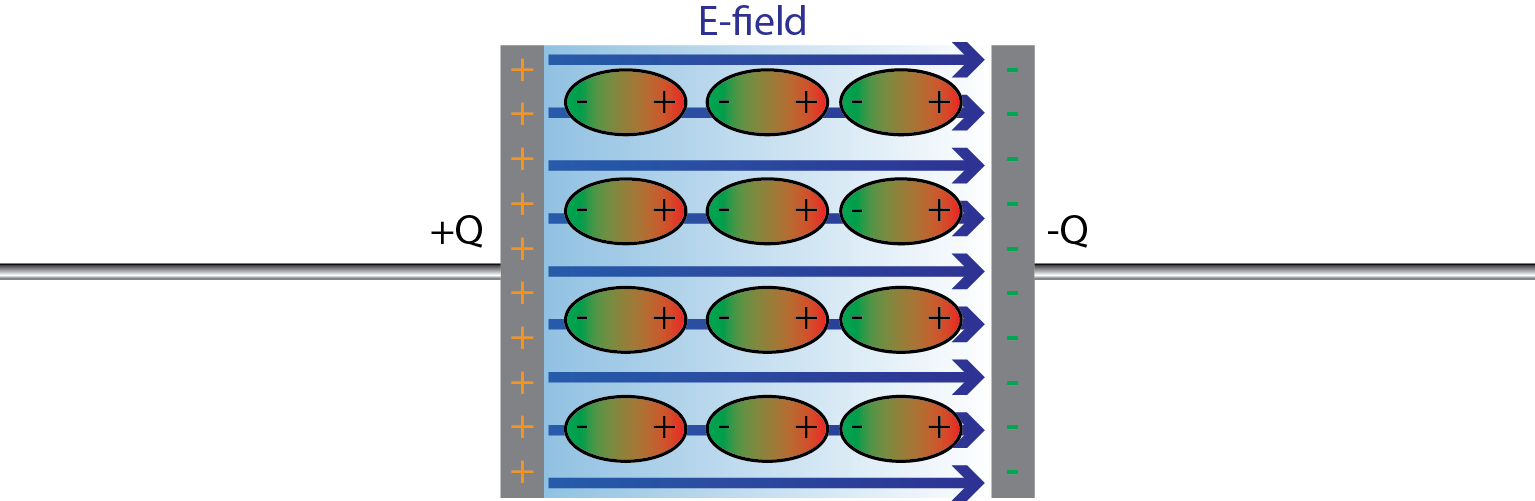
\includegraphics[width=\textwidth]{capcartoon.png}
\end{center}
\end{figure}


It is interesting to consider the physics of the insulating dielectric in an electric field. Although by definition no current can flow, the atoms and molecules in the dielectric will align themselves in such a way that minimizes the energy of the system. This happens even in the simplest case of a Hydrogen atom which one might think of as spherically symmetric, as the electron and proton (wavefunctions) can have a net relative displacement. This polarization allows more charge to be stored for a fixed voltage and thus increases the capacitance of the device. At some point however, the electric field due to a high voltage will be sufficiently strong to rip electrons off of their cores and cause even an insulator to conduct. This effect, known as dielectric breakdown is what happens during a lightning storm for example, for which the dielectric breakdown voltage (of air in this case) is about 3,000,000 V/m. For practical capacitors, the breakdown is much lower. In the lab, note the rating of the capacitor (typically 35V, 200V etc) as exeeding this value can lead to dielectric breakdown (i.e. a loud ``pop'') and a ruined capacitor\footnote{In fact, ``blown'' capacitors are often the cause of fried computers, etc. The tell-tale trace is a capacitor with a puffed out lid where rapid internal heating due to the short caused thermal expansion}.

\section{Capacitors in a Circuit}

The circuit diagram for a capacitor is shown in figure \ref{fig:capz}a. Note that capacitors come in two distinct varieties: polarized and non-polarized. Polarized capacitors have an electrolytic layer which has a preferred direction. These capacitors have a marked ``-'' terminal. Current should always flow \textit{towards} this terminal, as reverse biasing can result in a shorted out capacitor.


\begin{figure}[h]
\caption{(a) Circuit diagrams for capacitors. (b) Hydraulic analogy. (c) Various Capacitors (Wikipedia).}
\label{fig:capz}
\begin{center}
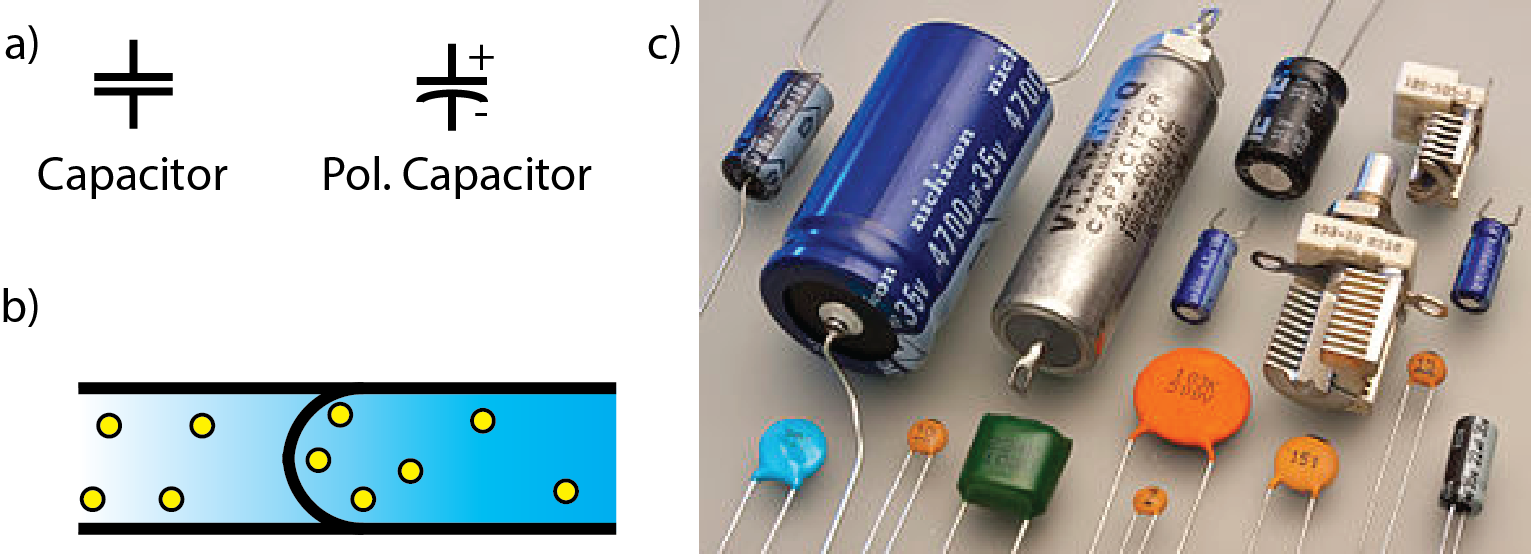
\includegraphics[width=\textwidth]{capz}
\end{center}
\end{figure}

\subsection{Parallel Combinations of capacitors}
In the same way as we did we can derive the effective capacitance of parallel and series combinations of capacitors. In this case, it turns out that parallel combinations are similar. To get a rough idea why, note that fro equation \ref{eq:capacitor_geom}, the capacitance is proportional to the area of the plates. A parallel combination of capacitors with  areas $A_1 $ and $A_2$ simply form a larger area, $A_1+A_2$ so that $C  = C_1+C_2$. More rigorously note that for a parallel combination, the voltages across each capacitor are equal. From the fundamental definition \ref{def:capacitance}, we have (using $i\equiv dq/dt$):

\begin{equation}\label{eq:cap_AC}
i(t) = C\frac{dV}{dt}
\end{equation}


\begin{align*}
i(t) &= i_1(t) + i_2(t) \\
C\frac{dv}{dt} &= C_1\frac{dv_1}{dt} + C_2\frac{dv_2}{dt} \\
C\frac{dv}{dt}&= \left(C_1+C_2\right)\frac{dv}{dt} \\
C &= C_1+C_2
\end{align*}

\begin{equation}\label{eq:parallel_cap}
\boxed{C_{\text{parallel}} = C_1+C_2}
\end{equation}


\begin{marginfigure}
\caption{Parallel and series combinations of capacitors.}
\label{fig:cap_netwerx}
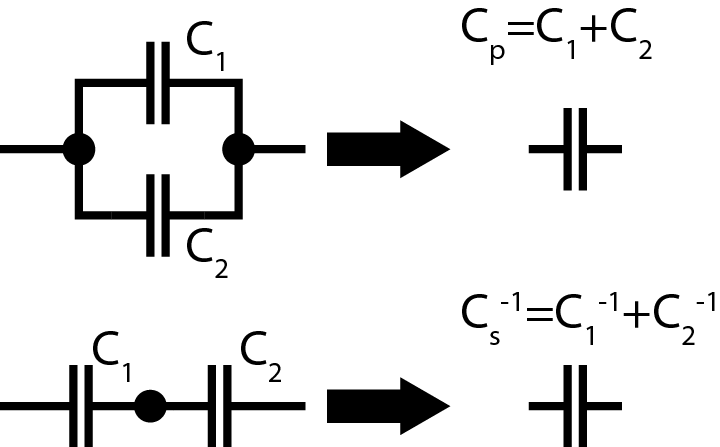
\includegraphics[]{cap_netwerx}
\end{marginfigure}

\subsection{Series Combinations of capacitors}
In a similar vein to the parallel case, we can derive the corresponding capacitance of a series combination. In this case, the current is constant so that:

\begin{eqnarray*}
i(t)  &= i_1(t) &= i_2(t) \\
C\frac{dv}{dt}  &= C_1\frac{dv_1}{dt}             &= C_2\frac{dv_2}{dt} \\
\frac{dv_1}{dt} &= \frac{C}{C_1}\frac{dv}{dt}  & \\
\frac{dv_2}{dt} &= \frac{C}{C_2}\frac{dv}{dt}  &
\end{eqnarray*}

\noindent Then, using $v(t) = v_1(t) + v_2(t)$, we have:


\begin{align*}
\frac{dv}{dt} &= \frac{dv_1}{dt} + \frac{dv_2}{dt} \\
\frac{dv}{dt} &= \left(\frac{C}{C_1}+\frac{C}{C_1}\right)\frac{dv}{dt}\\
\frac{1}{C}&= \frac{1}{C_1} + \frac{1}{C_2}
\end{align*}

\noindent Which is the law for a series combination of capacitors:

\begin{equation}\label{eq:series_cap}
\boxed{C^{-1}_{\text{series}} = C^{-1}_1+C^{-1}_2}
\end{equation}


\section{Energy stored in a Capacitor}
It turn's out that we can get a lot of mileage out of equation \ref{def:capacitance}. The first application is to determine the energy stored in a capacitor. Recall that the potential difference in a circuit is work done per charge $v = \frac{dW}{dq}$. We can calculate the energy stored in the capacitor by keeping track of the work done by charging an initially uncharged circuit from $0$ to $q$. By the work-energy theorem, the energy stored is just this work:

$$
E = \int_{q\prime=0}^{q} dW(q) =\int_{q\prime=0}^{q} v(q)dq = \int_{q\prime=0}^{q} \frac{q\prime}{C}dq\prime=\frac{1}{2}\frac{q^2}{C} 
$$

\noindent ... where we used equation \ref{def:capacitance} for the voltage. Re-using this equation to eliminate charge $q$, we have:

\begin{equation}\label{eq:energy_capacitor}
E_c=\frac{1}{2}CV^2
\end{equation}

\section{Discharging a Capacitor}

Consider the circuit on the lower left side of figure \ref{fig:chargedischarge}. Initially the voltage at all points in the circle is zero and there is no current. At some later time, a switch is closed connecting a battery with voltage $v(t) = V_0 =  \text{const}$. Current will thus immediately begin to flow and charge the capacitor. As the capacitor charges, we have learned that an electric field will build up which creates anEMF opposite that of the battery so the current will decrease as the capacitor charges until there is enough charge on the capacitor to create a voltage which is equal and opposite to the battery. The capacitor is then said to be charged -- we could yank it out of the circuit, stick it in out pocket and carry it across the room and it would still have that charge. Suppose we now close the switch disconnecting the battery but leaving a complete circuit. The voltage difference between the capacitors two terminals will drive current through the capacitor, decreasing the charge, fields and voltages in the process, until eventually, there is no net charge. This is called discharging the capacitor.

We can predict this behaviour more rigorously using by differentiating equation \ref{def:capacitance}:

$$
\frac{dq}{dt} \equiv i = C\frac{dv(t)}{dt}
$$

\noindent We can apply Kirchhoff's voltage rule to the closed circuit to deduce:

$$
v_{\text{batt}} -i(t)R - v_{\text{cap}}(t) = 0
$$

Combining both equations, we arrive at a differential equation for the voltage across the capacitor:


\begin{equation}\label{eq:cap_dif_eq}
v^\prime(t) =v_{\text{batt}} -\frac{1}{RC}v(t)
\end{equation}

Solving this equation tells us just how the voltage across the capacitor decays. For example, with a fully charged capacitor at $v_0$ when the switch is just closed. Equation \ref{eq:cap_dif_eq} now states

$$
v^\prime(t) =\frac{v(t)}{RC}
$$

\noindent The solution of this equation is:

\begin{equation}\label{eq:discharge}
v(t) = v_0e^{-t/RC} = v_0e^{-t/\tau}
\end{equation}

\noindent ... i.e. a simple exponential decay. The time constant 
\begin{equation}\label{eq:rctimeconst}
\tau = RC
\end{equation}
\noindent is known as the $RC$ (``are-see'')  time constant and will come up frequently in the material that follows.

\begin{figure}[h]
\caption{Charging and discharging a capacitor. Initially uncharged, a switch closes the circuit and the capacitor charges. The switch is then opened allowing the capacitor to uncharge.}
\label{fig:chargedischarge}
\begin{center}
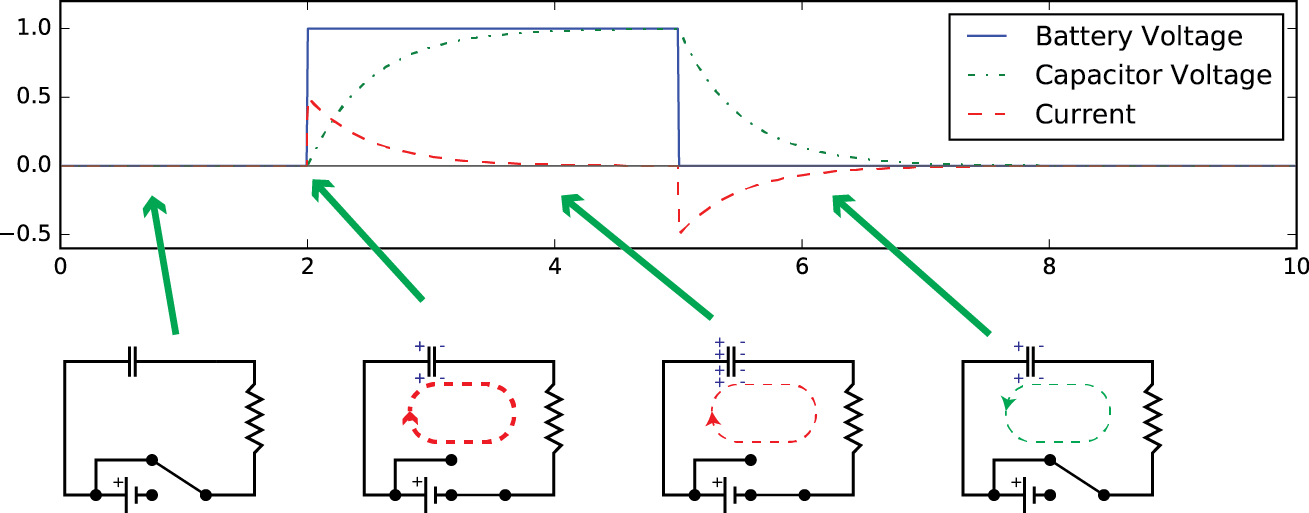
\includegraphics[width=\textwidth]{chargedischarge.png}
\end{center}
\end{figure}

\section{Supercapacitors}
Typical values for capacitance that you will encounter in the lab are pF, nF, $\mu$F, and mF. Even without a resistor connecting the terminals, the capacitor will discharge as current ``leaks through the dielectric''. This can be modelled as an large parallel resistance, forming an internal RC-circuit . A low leakage capacitor might have leakage times of seconds or even minutes, but it will eventually decay. In recent year, so-called supercapacitors or ``supercaps'' have been developed that have leakage times on the order of months and capacitance on the order of 10000F. This allows capacitors to be used in place of batteries.

\noindent Supercaps fall into several categories: From wikipedia:

\noindent\textbf{Electrostatic double-layer capacitors} use carbon electrodes or derivatives with much higher electrostatic double-layer capacitance than electrochemical pseudocapacitance, achieving separation of charge in a Helmholtz double layer at the interface between the surface of a conductive electrode and an electrolyte. The separation of charge is of the order of a few \r{A}ngstr{\"o}ms (0.3--0.8 nm), much smaller than in a conventional capacitor.

\noindent\textbf{Electrochemical pseudocapacitors} use metal oxide or conducting polymer electrodes with a high amount of electrochemical pseudocapacitance additional to the double-layer capacitance. Pseudocapacitance is achieved by Faradaic electron charge-transfer with redox reactions, intercalation or electrosorption.

\noindent\textbf{Hybrid capacitors}, such as the lithium-ion capacitor, use electrodes with differing characteristics: one exhibiting mostly electrostatic capacitance and the other mostly electrochemical capacitance.

The benefit of a supercap over a battery is that while it's energy storage is similar to a battery, it can be charged much, much faster and can survive many more cycles. Supercaps are already being used for energy harvesting, cordless tools, and regenerative braking systems for electric vehicles.

\section{Capacitors in AC Circuits}
We have seen that upon a sudden change in voltage, there is a lagged response of the current through a capacitor. What about the case of a continuously changing current, i.e. a sinusoidal voltage? We can see the effect of a sinusoidal voltage directly from equation \ref{eq:cap_AC}:

\begin{align}\label{eq:ac_cap_deriv}
i(t) &= C\frac{d}{dt}V_0\sin\left(\omega t\right) \nonumber\\
     &= \omega C V_0\cos\left(\omega t\right) \nonumber\\
     &= \omega C V_0\sin\left(\omega t + \frac{\pi}{2}\right)
\end{align}

\noindent Here we see two important properties: First, the current increases with frequency -- that is, there is somehow less effective resistance the higher the frequency. Second, there is a $90^\circ$ phase shift of the current with respect to the voltage.

Fortunately , we have already developed a beautiful formalism for dealing with phase shifts in sinusoidal signals, namely complex numbers. Using the fact that the RMS voltages of $\cos\omega t$ and $\sin\omega t$ are equal, we can rewrite \ref{eq:ac_cap_deriv} in terms of the RMS voltage across the capacitor. Recalling that from Euler's equation, we can write a $\pi/2$ phase shift as $e^{j\pi/2} = j$:

\begin{equation}\label{eq:cap_impedance}
V_C = I\left(\frac{-j}{\omega C}\right) \equiv IZ_C
\end{equation}

Thus we can treat the response of a capacitor in an AC circuit as sort of generalized resistor obeying Ohm's law with complex, frequency-dependant resistance, known as the \textit{impedance}, denoted $z$. Impedance is an important topic to which we will return shortly.

\section{Inductance}
We have just seen that capacitors provide an impedance which decreases with frequency, varying inversely ($\vert Z \vert \propto \omega^{-1}$). In the process, they store energy in the electric field. There exist another class of components known as \textbf{inductors} whose impedance increases linearly with frequency and function by storing energy in the magnetic field.

The physics of an inductor stems from the phenomenon of self-inductance. Recall that Faraday's law of induction states that a change in flux of a magnetic field through a circuit will result in an EMF which is given precisely as the time derivative of a magnetic field. Recall also that the Biot-Savard law states that whenever a current passes through a wire, a rotational magnetic field is formed around the wire. When current is passed through a wire wound coil, a large magnetic field is created (Biot-Savard law), and this in turn creates an EMF which opposes the current (Faradays law). This phenomenon is know as ``self-inductance''.

An inductor is thus merely a wire bend into a geometry which creates a given flux for a given current. Often the coil is wrapped around a ferromagnet to increase the magnetic flux. Since Biot-Savard law gives us a direct relation between magnetic flux and current, we can write characterize the effect of an inductor in terms of currents and voltages, bypassing descriptions of electromagnetic fields, as in equation \ref{def:capacitance}:

\begin{equation}\label{def:inductance}
v(t) = L\frac{di(t)}{dt}
\end{equation}

\noindent The constant $L$ is known as the ``inductance'' and depends entirely on the geometry of the inductor. The units of inductance are the \textit{Henry} H. Typical values are in the range of 1~mH to 1~H. The use of a ferromagnetic substance such iron increases the inductance significantly.

\begin{figure}[h]
\caption{(a) Parallel and series combinations of inductors follow the same rules as resistors. (b) Hydrostatic analogy of an inductor: a heavy turbine with inertia. (c) Various inductors. Lower is an ``RF choke'' use to filter spikes and other high frequeuncy noise.}
\label{fig:inductors}
\begin{center}
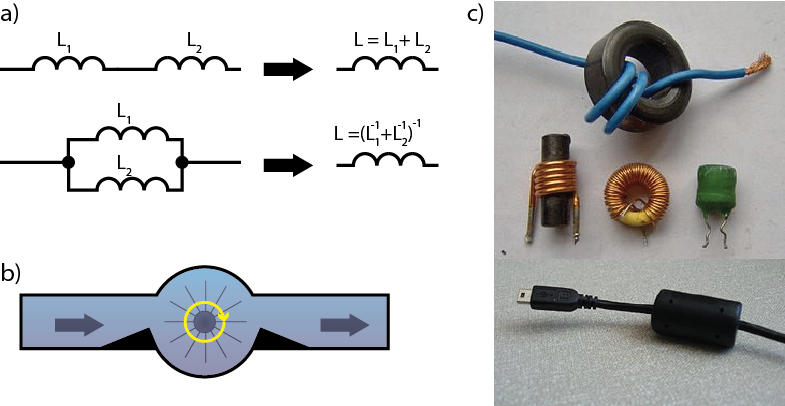
\includegraphics[width=\textwidth]{inductee.png}
\end{center}
\end{figure}

We can ask what the response of an inductor is to a sinusoidal input voltage in the same way as we did with capacitors. With equation \ref{def:inductance} as our guide, we see that when $v(t) = A\sin\omega t$ we have

$$
L\frac{di(t)}{dt} = A\sin\omega t
$$

\noindent which when integrated gives

\begin{equation}\label{eq:ind_deriv}
i(t) = i_0 -\frac{1}{\omega L}\cos\omega t = i_0 +\frac{1}{\omega L}A\sin\left(\omega t  -\frac{\pi}{2}\right)
\end{equation}

\noindent Equation \ref{eq:ind_deriv} tells us two important points. First, the current through an inductor thus \textbf{lags} the voltage by $90^\circ$. Second, in terms of RMS quantities, we have $v_\text{RMS} = \left(\omega L\right)i_\text{RMS}$. Thus, the response of the inductor is:

\begin{equation}\label{eq:impedance_inductor}
V_L = I\left(j\omega L\right) = IZ_L
\end{equation}

\section{Impedance and Reactance}
We have seen that the current across a resistor is in phase with the applied voltage such circuits are known as ``resistive''. On the other hand, current across a capacitor or inductor is $90^\circ$ out of phase with the voltage and are known as ``reactive'' components. The significance of reactive components is that since their current is always perfectly orthogonal (i.e. $\pm90^\circ$ out of phase) with respect to the voltage, they dissipate no power. This stems form a generalized version of power dissipation: $P = \int_T i(t)v(t)dt$. 

Consider an input of $v(t) = A\sin\omega t$. For a resistor, $i(t) = v(t)/R$

$$
P = \int_0^{t=T} i(t)v(t)dt = \frac{A^2}{R}\int_0^{2\pi/\omega} \sin^2\omega t = \frac{A^2}{2R} = \frac{v^2_\text{RMS}}{R}
$$

\noindent On the other hand, for a capacitor or inductor we have $i(t) = \kappa\cos\omega t$ (with $\kappa$ depending on whether we have a capacitor or inductor. In this case:

$$
P = A^2\kappa\int_0^{2\pi/\omega} \sin\omega t\cos\omega t = \frac{1}{2}A^2\kappa\int_0^{2\pi/\omega}\sin2\omega t = 0
$$

The magnitude of the impedance is known as the reactance $X$ -- there is no information with respect to the impedance, but it merely neglects the phase information. The impedance reactance and phase information is summarized in table \ref{tab:impedance}.

\begin{table}[h]
\caption{Impedance and Reactance of various components}
\centering
\label{tab:impedance}
\begin{tabular}{|c|c|c|c|} \hline
Circuit Element & Impedance, Z & Reactance, X & Phase  \\ \hline \hline
Resistor & $R$ & $R$ & $0$ (in-phase) \\ \hline
Capacitor & -$\frac{j}{\omega C}$ & $\frac{1}{\omega C}$ & $-\frac{\pi}{2}$ (lags) \\ \hline
Inductor & $j \omega L$ & $\omega L$ & $\frac{\pi}{2}$ (leads) \\ \hline
\end{tabular}
\end{table}


\section{Leading, Lagging and Transients}
We have seen that resistors exhibit no phase shift, inductors have a positive phase shift and capacitors have a negative phase shift. How do we interpret this in terms of what happens to a sine wave input? Recall that when plotting any function of time $y(t)$, replacing $y(t) \rightarrow y(t+\Delta t)$ merely displaces the whole plot to the left (i.e. to an earlier time) by $\Delta t$. To see why this is note that the new function will always take the same value as the old one $\Delta t$ (seconds) earlier: at $t=-\Delta t$, we get $f(-\Delta t + \Delta t) = f(0)$. If $\Delta t = 5$, at $t=21$ we get $f(26)$ and so forth. Similarly, a negative phase shift is to the right and to a later time.

\begin{figure}[h]
\caption{Leading corresponds to a shift to the left (sooner in time) while lagging shifts a trace to the right (later in time).}
\label{fig:leadlag}
\begin{center}
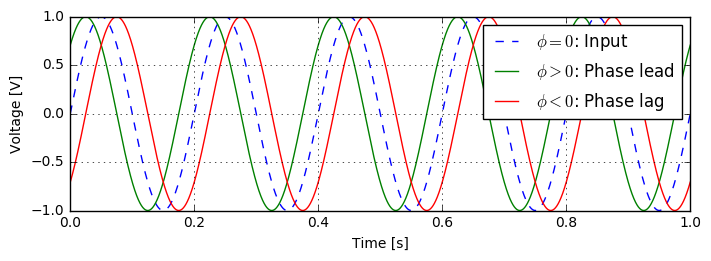
\includegraphics[width=\textwidth]{leadlag.png}
\end{center}
\end{figure}

In electronics, we then speak of time delays and phase shifts synonymously. When a current or voltage experiences a positive phase shift, we say that it ``leads'' the input. When it experiences a negative phase shift, it ``lags'' the input. This is illustrated in figure \ref{fig:leadlag}.

\noindent To relate the phase shift of a sine wave to a time delay, we merely write:

\begin{align}\label{eq:phase_time_sine_1}
v(t) &= \sin\left(\omega t + \phi\right) \nonumber\\
     &= \sin\left(\omega\left(t + \frac{\phi}{\omega}\right)\right) \nonumber\\
     &\equiv \sin\left(\omega\left(t + \Delta t\right)\right) 
\end{align}

\noindent i.e. A phase shift $\phi$ of a sine wave of frequency $\omega$ corresponds to a time shift:

\begin{equation}\label{eq:phase_time_sine_2}
\Delta t_{f,\phi} = \frac{\phi}{\omega}
\end{equation}

One thing you may find unnerving is how the output could ever \textbf{lead} the input - a notion that at first seems to defy causality. The answer to this riddle is that what we have discussed so far is the so-called ``steady state responses'' - that is, the input-output relations after the circuit has been left on for some time. Mathematically, the steady state is only exact after an infinite time but fortunately in practice it is sufficiently accurate after several periods. The response of the system when is it is first switched on is called the ``transient behaviour'' of the system. In fact, when you study differential equations such as those describing the resistor and capacitor circuits you will find that the solution to these equations can be written as a sum of steady state and transient responses. Below, I've plotted the solution to equation \ref{eq:cap_dif_eq} but with a sinusoidal input in place of the constant battery voltage. Note that the leading steady state response of an RC circuit is established during the initial transient response. Causality is safe


\begin{figure}[h]
\caption{Transient response of a leading output circuit.}
\label{fig:RC_transient}
\begin{center}
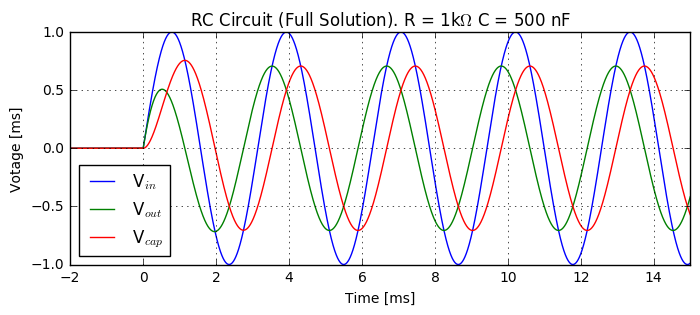
\includegraphics[width=\textwidth]{RC_transient.png}
\end{center}
\end{figure}


\section{Impedance-Based Voltage Dividers: Frequency Filters}
So far, we have studied how individual components, such as resistors, capacitors, and inductors respond to sinusoidal inputs. We have seen that that in terms of the RMS amplitudes, inductors and capacitors form ``frequency dependant resistors''. We will now study circuits with a mix of reactive and resistive circuits which can exhibit much richer behaviour.

Recall that when when we combined resistors in a voltage divider configuration, we could create an arbitrary voltage gain based on the values of these resistors. By combining several component types in a voltage divider configuration, we can now make an voltage dependant on frequency. 

\begin{figure}[h]
\caption{(a) Generalized impedances can be combined to form a voltage divider. (b) RC ``Low-Pass'' filter. (c) RL ``High Pass'' filter.}
\label{fig:cpx_volt_div}
\begin{center}
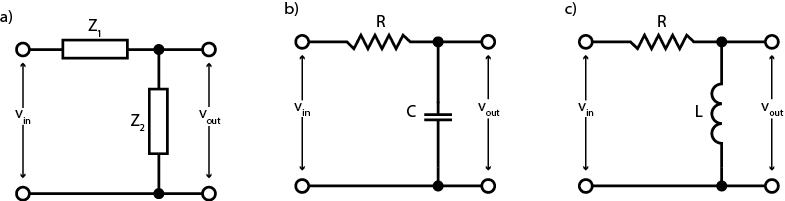
\includegraphics[width=\textwidth]{cpx_volt_div.png}
\end{center}
\end{figure}

Based on our previous analysis, we see that we can immediately replace the ``R's'' with ``Z's'' and we have the equation for the complex voltage divider:


\begin{equation}\label{eq:cpx_volt_div}
\frac{v_\text{out}}{v_\text{in}} \equiv G(\omega) = \frac{Z_2}{Z_1 + Z_2}
\end{equation}

\noindent We will now look at a few specific examples.

\subsection{RC ``Low-Pass'' filter}
Observe the circuit in figure \ref{fig:cpx_volt_div}b. Here, $Z_2 = -j/\omega C$ and $Z_1$ is merely $R$. Simpleminded substitution into equation \ref{eq:cpx_volt_div} gives:

$$
G(\omega) = \frac{-j/\omega C}{R - j/\omega C} 
$$

\noindent Multiplying top and bottom by $j\omega C$:

$$
G(\omega) = \frac{1}{1+j\omega RC}
$$

\noindent We see why this is called a ``low-pass'' filter: For DC signals ($\omega \rightarrow 0$) the gain is unity, i.e. $v_\text{in} =  v_\text{out}$. For very high frequencies ($\omega \rightarrow \infty$) the $\omega^{-1}$ dependance dominates and the gain tends to 0. 

Recall that the gain in our formalism is a complex quantuty and thus the circuit provides both an attenuation and a phase shift, to get a better grip, we often talk of the \textit{magnitude} and \textit{phase} of the filter. Applying our now-expert skills in complex numbers:

$$
\vert G(\omega)\vert = \sqrt{GG^*} = \sqrt{\left(\frac{1}{1+j\omega RC}\right)\left(\frac{1}{1-j\omega RC}\right)}
$$

or

\begin{equation}\label{eq:mag_RCLPfilt}
\vert G(\omega)\vert  = \frac{1}{\sqrt{1+\left(\omega R C\right)^2}}
\end{equation}


\noindent To get the phase, we can split this into real and imaginary parts by multiplying top and bottom by the complex conjugate of the denominator:

$$
G(\omega) = \frac{1-j\omega RC}{1+\left(\omega RC\right)^2} =  \frac{1}{1+\left(\omega RC\right)^2} - j \frac{\omega RC}{1+\left(\omega RC\right)^2}
$$

\noindent The phase of the filter is thus given by $\tan\phi = \Im\text{m}G/\Re\text{e}G$:

\begin{equation}\label{eq:phs_RCLPfilt}
\phi(\omega) = -\tan^{-1}\omega R C
\end{equation}

\noindent Note that for DC signals the phase shift $\phi = 0$ and for high frequencies, $\phi \rightarrow -\pi/2$.

We see that everything is characterized by the quantity $R\omega C$. When $R\omega C \approx 1$ the amplitudes begins to roll off and the phase is halfway between its extrema. We call the frequency at which this happens the \textbf{cut-off frequency} $f_\text{co}$:

\begin{equation}\label{eq:f_cutoff_RC}
f_\text{co} = \frac{1}{2\pi}\frac{1}{RC}
\end{equation}

\noindent Note that at the cutoff frequency, the magnitude of the transfer function is $1/\sqrt{2}$. The inverse of this quantity is sometimes called the ``RC time constant''.

\subsection{RL ``High-Pass'' filter}
Now, consider the circuit in figure \ref{fig:cpx_volt_div}c. Here, $Z_2 = j\omega L$ and $Z_1$ is again $R$. The voltage divider equation gives

$$
G(\omega) = \frac{j\omega L}{R+j\omega L}
$$

In the same way as before we find the magnitude of this filter to be:

\begin{equation}\label{eq:mag_RLHPfilt}
\vert G(\omega)\vert  = \frac{\omega L/R}{\sqrt{1 + \left(\omega L/R\right)^2}}
\end{equation}

\noindent Note that this serves as the counterpart to the previously mentioned low-pass: as $\omega \rightarrow 0$, the gain drops to 0 whereas as $\omega \rightarrow \infty$, $G(\omega) \rightarrow 1$.

\noindent Setting the output to $1/\sqrt{2}$, we find the cutoff frequency to be

\begin{equation}\label{eq:f_cutoff_RL}
f_\text{co} = \frac{1}{2\pi}\frac{R}{L}
\end{equation}

\noindent The phase is:
\begin{equation}\label{eq:phs_RLHPfilt}
\phi(\omega) = \tan^{-1}\frac{R}{\omega L}
\end{equation}

\noindent... which ranges from $\pi/2$ at DC to $0$ for $f\gg f_\text{co}$.

\section{Frequency Response and Bode Plots}
We have just seen that for a particular sine wave of a particular frequency, there is a particular phase shift and attenuation. Recall from section \ref{sec:fourier} that any signal can be broken down into a weighted sum of sine waves of a given amplitude and phase. It then makes sense to look at out frequency filters in the frequency domain. The behaviour of a device for all frequencies is known as the \textit{frequency response} of the system. We have already seen two frequency responses (namely of a RC low-pass and RL high-pass filter.

Since there is typically such a broad range of frequencies and signal levels, it is common (and useful!) to plot the frequency response logarithmically, producing what is called a \textbf{Bode Diagram}. First, it may be useful to recall some common properties of logarithms. 

\subsection{Logarithms}
There are a multitude of such properties  but we will stick here only to what is immediately relevant. First the definition of a logarithm is as the inverse of exponentiation:

\begin{equation}\label{eq:deflog}
b^x = y \Leftrightarrow \log_by = x
\end{equation}

\noindent Here $b$ is called the base of the logarithm. The most common logarithms are base 2 (if you're a computer scientist), base 10, (if you're an engineer,) and base $e$ (if you're a physicist). Recall that $e = 2.718\ldots$ is the natural number. When the base is not explicitly stated it is taken to be base 10. Log base $e$ is called the ``natural logarithm'' and is given a special symbol: $\log_ex\equiv \ln x$. 

Logarithms are useful for at least two reasons. First, they can convert certain mathematical operations to easier ones: Since $\left(y^x\right)^n = y^{nx}$ we have:

\begin{equation}\label{eq:logexp}
\log x^n = n\log x
\end{equation}

\noindent Also, since $ x^ax^b = x^{a+b}$, we have

\begin{equation}\label{eq:logmult}
\log\left(AB\right) = \log A  + \log B
\end{equation}

This leads to the second useful property of logarithms: they allow one to visualize a wide array of frequencies on a single plot. When plotting the x axis logarithmically, we can ``zoom in'' across many different scales where each division is an order of magnitude. Often there is interesting stuff happening in the low frequency range - say from 1~Hz to 100~Hz and also in the high frequency region, from 1~MHz to 1~GHz, say. It would be impossible to visualize this on a linear scale but logarithmically it is a simple task. Such a plot is called a ``semi-log plot''. It also is useful to make so-called ``log-log'' plots where both x and y are plotted logarithmically. As an example, consider an inverse-square law:

$$
f = \frac{1}{r^2}
$$

On a log scale, this reads:

$$
\log f = \log(r^{-2}) = -2\log(r)
$$

\noindent Letting $F\equiv\log f$ and $R\equiv\log{r}$, this reads

$$
F = -2R
$$
\noindent Thus, on a log-log plot, power laws become linear relationships for which the slope is the power.


\begin{figure}[h]
\caption{Log-Log 'Bode' plot of the function $f(x) = 0.1x^{-1}+x^{-2}$. Note that in the log-log plot, the point at which the $x^{-2}$ dependance dominates is clear where in the linear case, it is not.}
\label{ fig:BodePowers}
\begin{center}
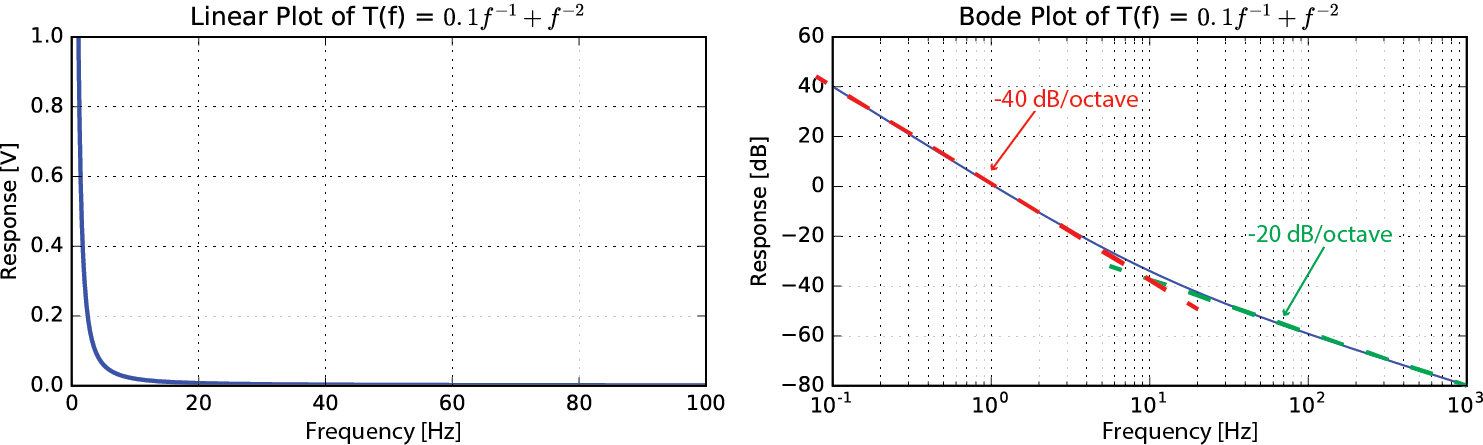
\includegraphics[width=\textwidth]{BodePowers.png}
\end{center}
\end{figure}


\subsection{Decibels}
You are likely already familiar with a logarithmic scale - the so-called decibel scale used for hearing. In electronics decibels are also used frequently. The definition we use is as follows for a number\footnote{Note that like exponents and sines, the argument of a logarithm is necessarily unit-less} N:

$$
N_\text{dB} = 20\log_{10}N
$$

This definition gives rise to the fact that for every power of 10, we add 20 dB. A few sample calculations will be instructive:


\begin{align*}
|v_o/v_i| &= 1 \rightarrow G=0~\text{dB} \\
|v_o/v_i| &= 10  \rightarrow G=+20~\text{dB} \\
|v_o/v_i| &=0.1 \rightarrow G=-20~\text{dB}\\
|v_o/v_i| &= 1/\sqrt{2} \rightarrow G\approx -3~\text{dB}
\end{align*}

The significance of -3~dB is as follows. Recall that from power \ref{eq:joule_ohm} that the power drop across a load is given by $P = V^2/R$. When the power has dropped by 1/2, the voltage drop has decreased by a factor of $1/\sqrt{2}$ and thus by 3~dB. The ``3-dB'' point is common in the nomenclature of filters which fall off at a given point, as you will recall from high- and low-pass filter analysis.

\subsection{Bode Plots}
The frequency response (in dB) and phase (in either degrees or radians) plotted on a semilog scale is known as a Bode plot. The utility of Bode plots are that the cutoff frequency, roll-off and phase shifts are clearly visible. Figure \ref{fig:bode_filts} displays Bode plots for high and low pass filters.


\begin{figure}[h]
\caption{Bode Plots for high and low pass filters discussed above.}
\label{fig:bode_filts}
\begin{center}
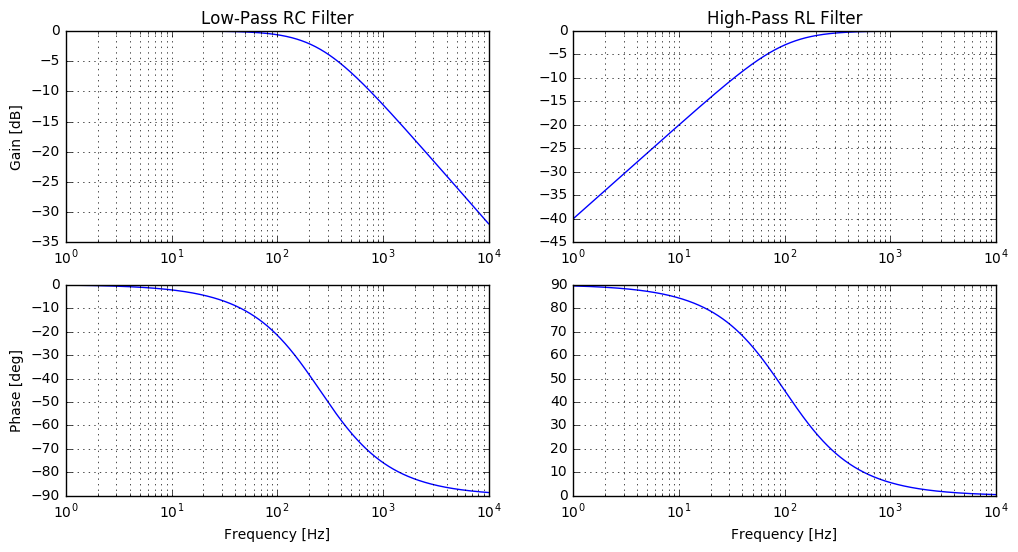
\includegraphics[width=\textwidth]{bode_filts.png}
\end{center}
\end{figure}

%%% ========================================================
\chapter{Semiconductors and Diodes}
The circuit we have studied thus far have all fallen under the regime of ``linear, passive components''. \textit{Linear} means, essentially that if we send in a sine wave, at frequency $\omega$, the output is also a sine wave, but perhaps at a different amplitude and with a different phase\footnote{A more general definition of linearity is as follows: Suppose that, given inputs $v_1^{in}$ and $v_2^{in}$, our device $D$ produces outputs $v_1^{out} = Dv_1^{in}$ and $v_2^{out} = Dv_2^{in}$. We say $D$ is a linear device if, when we send the sum of the inputs $v_3^{in} = v_1^{in} + v_2^{in}$, then the output is the sum of the individual outputs: $v_3^{out} = Dv_3^{in} =  v_1^{out} + v_2^{out}$}. \textit{Passive} means that the device does not require additional power in order to function. We will deal with non-passive devices next chapter. This chapter we will encounter our first non-linear device, namely the diode. We'll start by defining what we want out of a diode, and then move on to how to actually make one. In order to consctruct a diode we will make use of a new class of materials: ``semiconductors'' which under various circumstances behave like a conductor, an insulator, or neither.

\section{The Ideal Diode}
Before we go on to describe how to build a diode, which involves a fairly hefty diversion into solid state physics, let's incentivize ourselves to learn by describing what we could do should we have one. 

\begin{marginfigure}%
  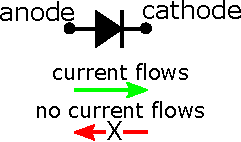
\includegraphics[]{diodecurrentflow}
  \caption{The circuit symbol for a diode. The direction of current flow is the way the ``arrow'' points.}
  \label{fig:diode_sym}
\end{marginfigure}

The basic diode circuit is shown in figure \ref{fig:diode_sym}. A diode is essentially a one-way valve for current. If we pass current from terminals $a$ to $b$, the diode acts as a short circuit (ie. a wire). If we try to pass current the other way the diode acts as an open circuit and no current passes. The resistance is thus assymetric: $R_{ab} = 0~\Omega$, $R_{ba} \rightarrow \infty$

The simplest reason to build use a diode is circuit protection. Many devices\footnote{You've already come across electrolytic capacitors which can be destroyed if reverse biased. Another example is pizoelectric stacks which expand nicely in forward bias but self destruct in reverse bias.} can be damaged if you try to run current through it in the wrong direction. 

Another important used of diodes is signal rectification which you will explore in the lab. Suppose that we want to run current through some load (whatever it is) in one direction only. If we merely place a diode at its input current flows through the positive phase of an ac signal but is blocked for the negative phase (figure \ref{fig:rect_half_full}a). Since no current flow during this phase, no power is wasted. 

A shortcoming of the half-wave rectifier is that we are only using half the signal. Power is \textit{delivered} to the load during the positive half-cycle in between half-cycles of nothing. To make use of the entire signal, a clever topology shown in figure \ref{fig:rect_half_full}b can be employed. During the positive cycle, the current takes enteres the top junction and sees only the path on the right, leading to the load. On the return path, the diode on the bottom left leads back to the source. On the negative half cycle, current flows from the bottom node through the load and up the top.

\begin{myexample}[label = ex:welches_wegen_diode]{Pop Quiz!}
Why doesn't the current go back through the load through the right diodes on the return path?
\end{myexample}

\begin{marginfigure}%
  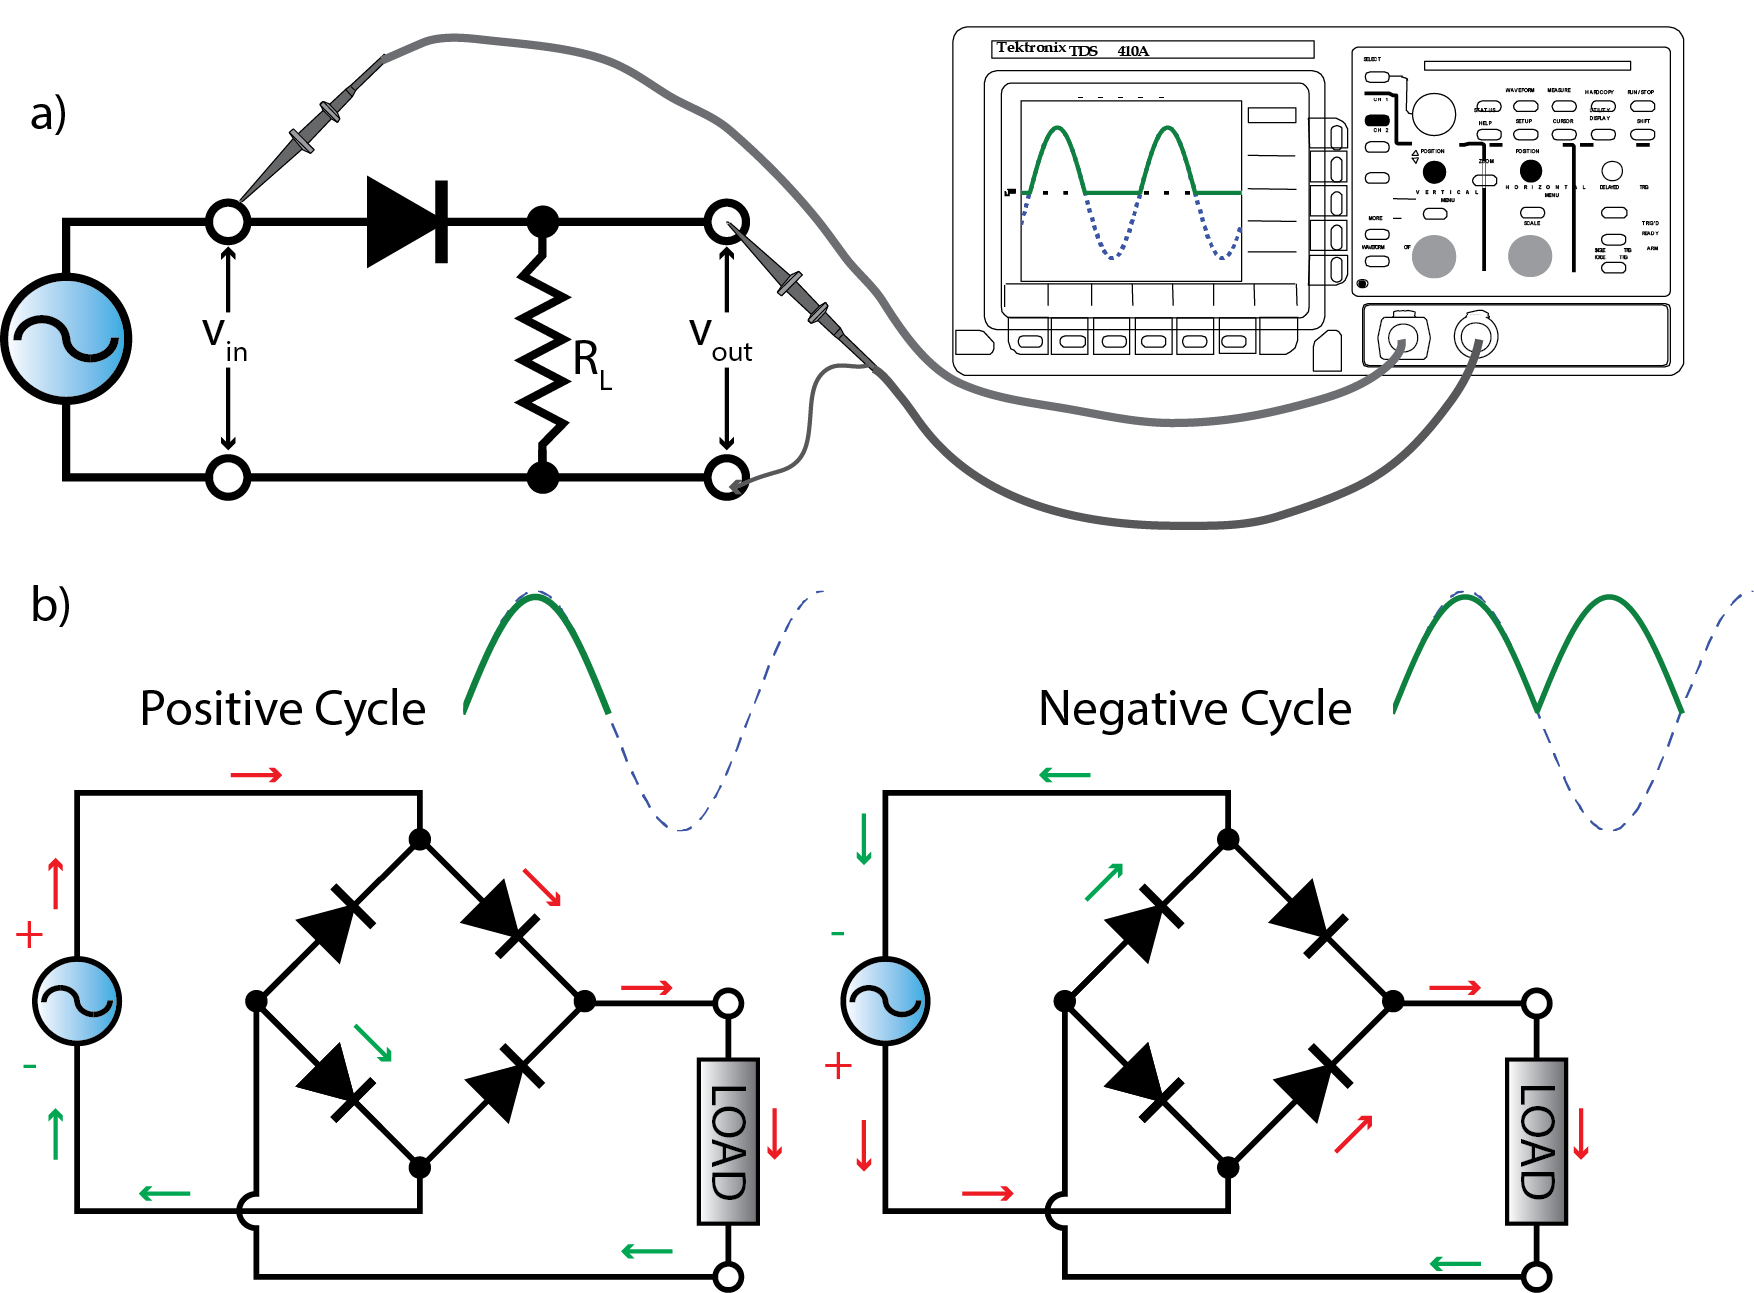
\includegraphics[]{rectification_half_full}
  \caption{a) Half wave rectifier. b) Full wave rectifier. Note that regardless of the polarity of the input, current flow is always in the same direction through the load.}
  \label{fig:rect_half_full}
\end{marginfigure}

By adding a smoothing capacitor across the load, this can be used as a "AC-adapter", converting the 60~Hz line voltage from the wall outlet to a DC signal. In lab 4, you will do just this.

OK now that we know a few of the useful applications of diodes (there are plenty more, some of which we'll mention soon), it's time to figure out how we'll actually build one. 

\section{Semiconductors}
In this course so far we've focused on two classes of materials: insulators (such as glasses or plastics) with very low conductivity and conductors (such as copper or silver) with very high conductivity. There is a third class of materials known as semiconductors whose behaviour can fall between the two extremes. Two common semiconductor materials are Silicon and Germanium. On their own Si and Ge semiconductors form crystals exhibiting somewhat interesting behaviour, but by adding trace amounts of impurity we can engineer fascinating technology allowing not only for the implementation of diodes, but of amplifiers, digital logic gates in computers, specialized detectors, and low power lights. A comprehensive understanding of semiconductor physics is too much of a diversion from our understanding of laboratory electronics (you'll have to wait a year or so for your solid state physics class) but this section will serve as a condensed crash course, outlining the basic idea of their functionality.

\subsection{A Microscopic Model of Conductivity: The Drude Model}

Take a metal such as copper, with a single valence electron in its outer shell, ($4s^1$ in this case.) In crystaline form, copper forms a metallic bond with its neighbors in which the valence electron is weakly bound to its ``original nucleus'' as compared to its nearby neighbors\footnote{ Apologies to any chemists reading this. That goes for this entire section...} and so a given electron can hop over to the atom next door. Of course, this would leave a positive charge and so another electron would quickly rush in to fill the gap. In this way, a metal has a ``sea of electrons'' bound to a lattice itself of positive centers, but not bound to any particular core. 

This picture of a conductor makes complete sense and explains well the phenomenon of conductivity -- until you stop to think about it too much. an immediate problem that arises is that if we connect a voltage across a conductor we should get a quadratically increasing current\footnote{Why? Because a voltage drop corresponds to a electric field: if we have a constantly decreasing voltage $V$ across a distance $d$, the definition of potential gives 
$$\vert E \vert = \vert\frac{dV}{dx}\vert = \frac{V}{d}$$ 
Since the force on a charge is $F = m\ddot{x} = qE$, we predict a constant acceleration of the current:
$$
\ddot{x}_e = \frac{qV}{m_ee}
$$
which is clearly not what is observed!}, whereas from experience (and Ohm's law) we get a steady, constant current.

An early attempt to resolve this conundrum was a model made by Paul Drude in 1900. Not only was Drude's model successful in forming a qualitative and quantitative description of conduction in a metal, it was able to explain why metals are good thermal conductors and insulators, tyically are not\footnote{It also explained a pressing problem of the day: the Hall effect which is seen when a magnetic field is sent parallel to the current. Experimentally a voltage perpendicular to both the current and magnetic field was measured}. Unfortunately, the Drude model is also wrong - it fails to tke in statistical effects on electrons \footnote{Namely the Pauli Exclusion Principle}, the temperature dependance of conctivity, and get the numbers very, very wrong for certain substances. That being said, it is surprisingly accurate for most materials and lets us apply an intuitive picture to the nuts and bolts of electronic quantities that is not too far off the mark. For this reason, it is still taught before more recent theories which are more correct, more sophisticated, and more difficult to understand. 

The drude model makes the following assumptions:

\begin{enumerate}
  \item A conductor consists of heavy, immobile, positively charged centers surrounded by a gas of light electrons.
  \item Electrons do not interact with one another or with the \textbf{fields} of the ionic cores\footnote{This is known as the independant-electron and free-electron approximations, respectively}.
  \item Electrons thus travel in straight lines for a mean time $\tau$ between collisions with ionic cores. After collision, the electron has, on average a kinectic energy equal to the thermal equilibrium energy.

  \begin{equation}
    \label{eq:thermal_energy}
    E = \frac{1}{2}m_ev^2 = \frac{3}{2}k_BT
  \end{equation}
\end{enumerate}

It turns out that this is already enough to predict Ohm's law. In order to separate properties relevant to the conductor, rather than the shape of the wire, it is convenient to work with current density -- i.e. current per unit cross-sectional area, travelling in some direction $\hat{j}$:

\begin{equation}
\label{eq:current_density}
\textbf{j} = \frac{I}{A}\hat{j}
\end{equation}

Supposing that our conductor has $n_v$ valence electrons per atom and a density of $N$ atoms per unit volume\footnote{The usual symbol $\rho$ is already spoken for in this context.}, we can relate the current density to the average velocity as:

\begin{equation}
\label{eq:current_density_velocity}
\textbf{j} = -Nn_ve\textbf{v}_\text{av}
\end{equation}

Note that although the electrons have a non-zero average \textit{speed} according to eq. \ref{eq:thermal_energy} they are equally likely to be travelling in any direction. Thus the average \textit{velocity} and therefore current is zero. However, if we apply a voltage difference, and therefor an external field $\textbf{E}$ across the connductor, the electrons will experience a constant acceleration between collisions given by:

\begin{equation}
\label{eq:coulomb_accel}
\textbf{a} = -\frac{e\textbf{E}}{m_e}
\end{equation}

\noindent... before being re--randomized. There will thus be an average velocity which will \textit{not} average out, given by\footnote{Since $v_f = a\tau$ and $v_i = 0$, $v_\text{av} = \frac{1}{2}a\tau$}:

\begin{equation}
\label{eq:drude_avg_velocity}
\textbf{v} = \frac{a\tau}{2} = -\frac{eE\tau}{2}
\end{equation}

\noindent\ldots and the current density, eq. \ref{eq:current_density}, is therefore:

\begin{equation}
\label{eq:drude_ohms}
\textbf{j} = \left(\frac{Nn_ve^2}{2m_e}\right)\textbf{E} \equiv \sigma\textbf{E}
\end{equation}

\noindent\ldots which \textbf{is} Ohm's law: namely that current is proportional to the Electric field. The constant of proportionality $\sigma$ is the conductivity from chapter 1 (i.e. the inverse of the resistivity $\rho = \sigma^{-1}$). Of course, that is not how we normally write Ohm's law. To see that it is indeed equivalent recall two facts: 
\begin{enumerate}
  \item Resistance through a chunk of material with resistivity $\rho$, cross-sectional area $A$ and length $L$ is $R = \rho\frac{L}{A}$.
  \item A uniform electric field throughout a region of length $L$ corresponds to a voltage $V = EL$
\end{enumerate}

Then, equation \ref{eq:drude_ohms} becomes:

$$
\textbf{j} = \frac{I}{A} = \frac{V}{\rho L}
$$

\noindent \ldots so that 

\begin{equation}
\label{eq:drude_ohms2}
V = I\left(\rho\frac{L}{A}\right) = IR
\end{equation}

Finally (for Physics 229 at least), we can predict use the mean free path of an electron to be rouhgly the interatomic spacing $l\approx a_0$\footnote{$a_0 \approx 0.5$~\AA~is the Bohr radius} and the fact that $l \approx v_\text{th}$ from equation \ref{eq:thermal_energy} to predict the temperature dependance of resistance. We will not go further with the Drude model -- you will get the chance in your solid state physics course, but we'll occasionally point to it when trying to understand the functionality of certain devices.

\subsection{Intrinsic Semiconductors: electons and holes}
Certain materials such as silicon are not metals\footnote{These are often classified as ``mettaloids'' on the periodic table} but can still under certain circumstances conduct electricity and are called \textit{semiconductors}. One such example, Silicon has 4 valence electrons (i.e. is tetravalent) and can form a tight lattice of covalent bonds with its four neighbors (see figure \ref{fig:SiLattice}). In this form these covalent bonds provide enough binding energy to localize the conduction electrons so that there is zero conductivity unless they are given extra energy. On the other hand, if we, through hook or crook, \textit{were} able to give tem more energy than this binding force, the electron would be free to zip around the crystal. This extra amount of energy required for a particular substance is called a ``band gap''\footnote{There is a lot we are glossing over here, but essentially, in a year or so you will learn about the ``band theory of materials''. If we plot the energy of an electrons that occupy the atom on a vertical, electrons in a Si atom just sitting around in their outer shell are in a range of energies called the ``valence band''. If they had enough energy to move freely, there would occupy the (first) ``conduction band''. The space between the two bands is thus called the band gap.}. 

\begin{marginfigure}%
  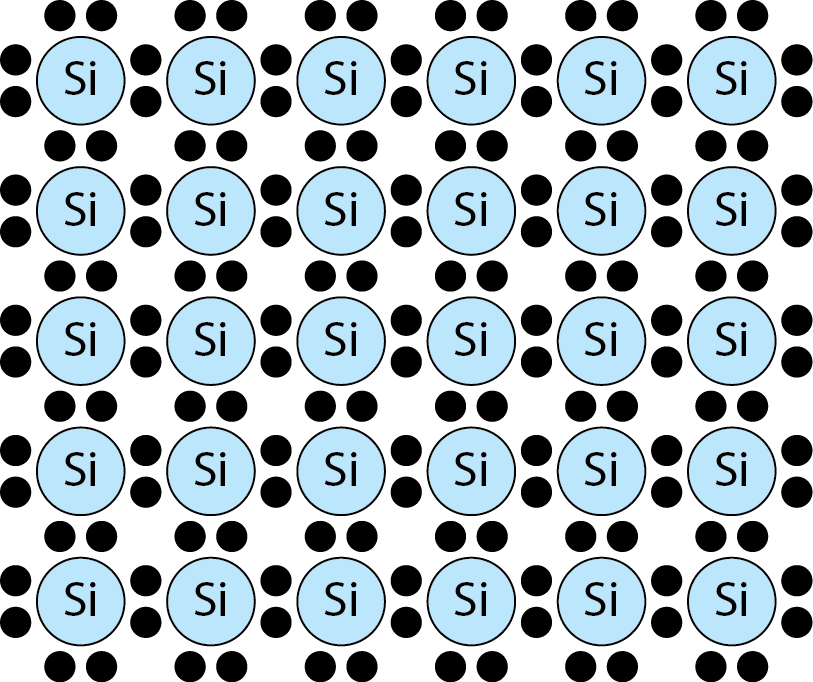
\includegraphics[]{SiLattice}
  \caption{Pure Silicon in crystalline form.}
  \label{fig:SiLattice}
\end{marginfigure}

The bandgap for typical semiconductors is typically on the order of an electron volt. For Silicon it is about 1.17~eV and for Germanim it is roughly 0.74~eV\footnote{... at very low temperatures. At higher temperatures the bandgap decreases slightly.}. What does this mean? It means that if you manage to give an electon a kick of extra energy equivalent to that it would get moving across 1.2~V, it would be freely moving along the solid. In doing so, it will leave a positively charged ``hole'' behind. An interesting consequence of these holes is that they behave identically to positive charge carriers propagating along the lattice. To see this consider figure \ref{fig:olez}. A neighboring electron can jump accross the small barrier into the positive hole. Similarly, another electron can jump into this newly formed hole. Although it is really the electrons moving around from atom to atom, the situation as a whole is as if there was a positively charged particle with charge $+q_e$ that is moving along the lattice. In semiconductor electronics we treat these holes as if they we real particles (sometimes we call them quasi-particles) and often speak of ``electron--hole pairs''.

How might we create electron--hole pairs? One way is to give an electron a boost by hitting it with a high energy photon. If we maintain a voltage across the Silicon, any free electrons will contribute to a current, giving roughly 1 electron per photon. This forms the basis of a type of light detector known as a photodiode.

Another way that an electron hole pair can be created is when the lattice imparts enough energy on its electrons via thermal vibrations. The mean energy is given by 
\begin{equation}
\label{eq:thermal_energy}
U_{th} = k_BT
\end{equation}
\noindent ... where $k_B$ is the Boltzmann constant $k_B \approx 1.38\times10^{-23}~\frac{\text{J}}{\text{K}}\approx 8.6\times10^{-5}~\frac{eV}{K}$. Of course, not every single particle has this exact energy, but are distributed according to the probability distribution:
\begin{equation}
\label{eq:thermal_distn}
Pr(E) \propto \frac{1}{1+e^{E/k_BT}}
\end{equation}

\noindent At room temperature, $k_BT\approx 1/40$~eV and there are enough free electron-hole pairs to make Si a reasonable conductor, while as $T\rightarrow0$~K, the number of free electrons vanishes. THus semiconductors thus have a resistance with very sharp dependance on temperature. 

What happens then when we increase the temperature significantly or bombard the semiconductor with photons? At some point there will be so many electron-hole pairs that it is very likely that many will collide. When this happens we say that the electron-hole pair annihilate one another in a phenomenon known as ``recombination''.

\begin{marginfigure}%
  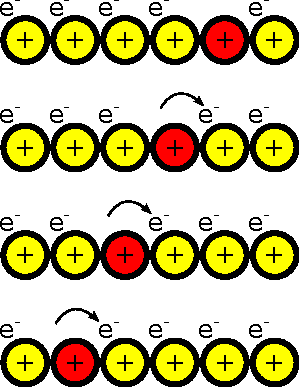
\includegraphics[]{jumpin_hole}
  \caption{At each step, an electron can ``jump'' into a neighboring site. This can be seen either as electrons shuffling to the right or a single \textit{hole} moving to the left.}
  \label{fig:olez}
\end{marginfigure}

\subsection{Extrinsic Semiconductors: N-type an P-type Doping}
Although the sharp temperature dependance of semiconductor conductivity is interesting, it is not terribly usefull in and of itself. First, temperature control within an circuit is a notorious pain and for the most part, you try to design circuits which are \textit{temperature insensitive}. Next, even if we take a blowtorch to our circuit the cinductivity remains too low to be very useful. Fortunately, nature has given us a very convenient trick known as \textbf{doping}.

Recalling that Silicon is tetravalent and forms these beautiful covalent bond-based lattices, we can try to put a similar atom \footnote{i.e. an atom that is nearby on the periodic table, and has roughly the same size.} If the atom is trivalent (three valence electrons) or pentavalent (5 valence electrons) the atom is still able to form the bond with the neighboring Silicon, but will have one fewer or one extra electron. For example, suppose we place a Phosphorous "impurity" atom, having 5 electrons in between a bunch of Silicon atoms. The impurity atom will fit right into the lattice and can use 4 of its 5 valence electrons to form a covalent bond with its neighbors. Of course it still has an extra electron kicking around and interesting, it will be heavily shielded from the shell. For example, whereas a single electron in a Hydrogen atom is held in a potential well of $-13.6$~eV, the extra Phosphorous electron will be held by a shallow $-0.1$~eV well, over 100 times less! This weakly bound electron will very easily leave its original home and wander freely through the lattice, leaving a small potential well behind. 

A similar picture exists for the holes in a trivalent atom such as Boron. The neighboring hole next to an atom corresponds to a very shallow energy gap and the electron has no problem acquiring enough energy to ``hop to the right'', or equivalently, the hole ``hops to the left'' (see figure \ref{fig:olez}).

The very shallow potential wells binding the electrons or holes leads to a constant diffusion of these charge carriers throughout the material. In the absence of and applied field, this diffusion is due to thermal jostling of the lattice and is the same in every direction yielding a net-zero current. Since these charge carriers are primarily responsible for any current, they are called the \textit{majority carriers} whereas the other charges are minority carriers. For example, in an N-type extrinsic semiconductor, the majority carriers are electrons and the minority carriers are holes. In a P-type semiconductor, the holes are the majority carriers and the remaining electrons are minority carriers.

A vast increase in extrinsic conduction can occur with a minute amount of doping. Typically the ratio of impurity to intrinsic atoms is anywhere between $10^{-6}$ to $10^{-9}$.

\subsection{PN Junctions}
The real magic occurs when a P-type and an N-type semiconductor are wedged against one another, creating a situation known as a \textit{PN junction}. This is diagrammed in figure [XXX]. Recalling that there is a constant diffusion of majority carriers in each semiconductures, 

\section{Semiconductor Diodes}
- TODO -
\section{Diode Circuit Analysis}
In circuit analysis using diodes, the details included in the Shockley diode equation are rarely of significance and we can use the simplified, step function approach. The key to analysis is as follows: if the potential placed across the diode is above the diode drop voltage $d_{dd}$, then the diode acts like an ideal EMF having potential difference $V = -V_{dd}$ opposing the current. If not, the diode acts like a voltage source equal and opposite the applied voltage:

\begin{equation}
\label{eq:effective_diode_source}
    V_{diode}=
    \begin{cases}
      -V_\text{in}, & \text{if}\ V\le V_\text{dd} \\
      -V_\text{dd}, & \text{otherwise}
    \end{cases}
  \end{equation}

The first question to ask is: will current flow. If so, then the amount of current that flows can be determined via Kirchhoff's laws.

\begin{marginfigure}
  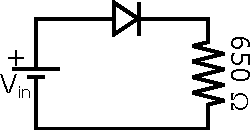
\includegraphics[]{simple_diode_ex}
  \caption{Simple diode example.}
  \label{fig:simple_diode_ex}
\end{marginfigure}


\begin{myexample}[label = ex:simple_diode]{Simple diode example.}
Determine the power dissipated in the resistor in figure \ref{fig:simple_diode_ex} for: $V_\text{in} = $ (a) 500~mV, (b) -3~V, and (c) 2~V. Assume that the diode voltage drop is 0.7~V.
\Solution
(a) Here we must determine if the voltage across the diode is greater that the voltage drop. You might see right away that the battery doesn't have enough kick, but we can formalise this. From Kirchhoff's laws the sum of the voltage dropped across the diode plus the voltage dropped across the resistor ($iR$) must sum to 0.5~V. The maximum voltage across the diode occurs when no current flows through the resistor (the diode then must drop all the voltage by it itself). In this case there si only 0.5~V dropped and by equation \ref{eq:effective_diode_source}, the diode acts like a -0.5~V battery. No current flows in the circuit and thpower dissipated in the resistor is zero.

(b) Here there is current being driven the opposite way. Again, current flowing across the resistor will only lessen the load on the diode and so there is, at zero current -3~V across the diode. Careful though! Although the magnitude is above $V_\text{dd}$ the direction is wrong - -3~V is certainly less than +0.7~V and so again by eq. \ref{eq:effective_diode_source} the diode acts like a battery with voltage +3~V, no current flows and so no power is dissipated.

(c) We begin the same way: If there is no current, the voltage across the diode is 2~V, which \textit{is} greater than $V_\text{dd}$. Finally, something interesting! Here, equation \ref{eq:effective_diode_source} tells us that the diode acts like a battery with $V=-0.7V$. From Kirchhoff's voltage law, the voltage across the resistor is then $V_R = 2~V-0.7~V = 1.3~V$. From Ohm's law, we see that there is $i = V_R/R = 1.3~V/650~\Omega = 2$~mA of current flowing through the circuit. The power dissipated in the resistor is:
$$
P = iV_R = \left(2.0~\text{mA}\right)\times\left(1.3~\text{V}\right) = 2.6~\text{mW}
$$

\textit{Bonus Question: How much power is dissipated in the diode?}
\end{myexample}

The previous example contains the essential way we think about diodes in this course. However we can easily come up with more complicated (but highly realistic) scenarios. For example, what happens when you place several diodes in series? In this case, each diode can drop at most $V_\text{dd}$ voltage before it starts conducting, but since each in series there is only one path for the current to take, there must be enough voltage left after the first voltage drop to overcome the remainder of the barriers. If you have an AC signal as an input, there can be times where the diode conducts and other times when it does not. In this case it helps to break the circuit up into cases. The next example shows how to del with some of these issues.


\begin{marginfigure}
  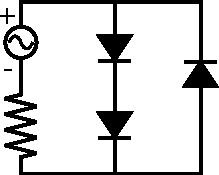
\includegraphics[]{less_simple_diode_ex}
  \caption{Less simple diode example.}
  \label{fig:less_simple_diode_ex}
\end{marginfigure}

\begin{myexample}[label = ex:less_simple_diode]{Less Simple diode example.}
Over what voltage range(s) does current flow in the circuit of figure \ref{fig:less_simple_diode_ex}? Assume that each diode has $v_\text{dd} = 0.7$~V.
\Solution
Here, we have an AC supply which can be either positive or negative (To remove ambiguity, we've labelled clockwise current as positive here.) Whenever the voltage is positive, there is no way that current will flow through the rightmost diode. The middle section \textbf{will} conduct whenever we have enough to overcome the potential barrier from both diodes. Here that is $2v_\text{dd} = 1.4$~V. Thus current flows when 

$$
V>1.4~\text{V}
$$
For negative voltages, the middle section always acts like an open circuit and current flows whenever the right most voltage has more than 0.7~V across it. Since this corresponds to counterclockwise current this is a negative voltage as per our labeling:
$$
V<-0.7~\text{V}
$$

Thus, abusing notation slightly, current flows whenever:
$$
-0.7~\text{V} > V > 1.4~V
$$

\textit{Bonus Challenge: Sketch the voltage dropped across the resistor and the total voltage on the same plot for a 4~V peak-to-peak sine wave.}
\end{myexample}

\subsection{Diode Based Rectification Circuits}
One of the primaray applicatitions of diodes is ``rectification''. Rectification basically means that we take an AC voltage and produce a DC voltage. More loosely, we take a voltage that can be positive and negative and produce an output that is purely positive\footnote{\ldots or purely negative.}. The simplest such circuit is the \textit{half-wave rectifier} shown in figure  XXX.
\section{Specialized Diodes}
- TODO -
\section{Sneek Peek Ahead: Transistors}
- TODO -
\chapter{Amplifiers}
\section{Active vs. Passive Circuits}
We now move into the regime of so-called \textit{active electronics}. Everything studied so far -- resistors and capacitors, to voltage dividers and filters, to diode rectifiers has fallen under the realm of passive electronics. Active electronic devices, in addition to standard inputs and outputs, require additional power supplies in order to function. There are great benefits to this, as we shall see: active components can output more power than at their input, and can eliminate annoying effects such as voltage loading due to input and output impedance. The first active device we'll study is the amplifier.
\section{The Ideal Voltage Amplifier}
The idea of the basic amplifier is simple: take the input $x_\text{in}$ and produce an output which is some number $G$ times the output.
\begin{equation}
\label{eq:simple_amp}
x_\text{out} = Gx_\text{in}
\end{equation}

\noindent ... where $G$ is known as the gain.

There is the question of what input $x_\text{in}$ is being amplified. In our course, normally $x_\text{in}$ will be a voltage and so we will have a voltage amplifier. In this case the gain is often expressed in decibels as:

\begin{equation}
\label{eq:voltage_amp_dB}
G_\text{dB} = 20\log\frac{v_\text{out}}{v_\text{in}} 
\end{equation}

We will occasionally deal with power amplifiers whose input and output is a power. For these amplifiers, the gain is also in dB but with a 10 instead of a 20 multiplier\footnote{Recall that for a fixed load resistance, $P = v^2/R \propto v^2$. Thus $10\log\left[P_\text{out}/P\text{in}\right] = 10\log\left[\left(v_\text{out}/v\text{in}\right)^2\right] = 20\log\left[v_\text{out}/v_\text{in}\right]$, thus yielding consistent definitions of gain}:

\begin{equation}
\label{eq:power_amp_dB}
G_\text{dB} = 10\log\frac{P_\text{out}}{P_\text{in}} 
\end{equation}

\noindent For now though, we will restrict ourselves to voltage amplifiers. Diagrammed in figure \ref{fig:simple_amp}. The output is described by equation \ref{eq:simple_amp}.

\begin{marginfigure}%
  \includegraphics[width=\linewidth]{SimpleAmplifier}
  \caption{The simplest of amplifiers: the output is the input multiplied by a constant gain $G$.}
  \label{fig:simple_amp}
\end{marginfigure}

\section{Reality Check: Amplifiers in Real Life}
There are several limitations to the ideal amplifier that come into effect in practice. For example the amplifier will have to draw at least a small current from the source in order to operate. As we've learned, this is equivalent to a finite \textit{input impedance} $R_\text{in}$. The amplifier will also have a limit to how much current it can output due to its internal resistances. This leads to a finite \textit{output impedance} $R_{out}$. There are also limits to how fast the amplifier can respond to a changing input signal. This leads to a finite \textit{gain bandwidth}, or in general, a frequency dependent gain $G(\omega)$. We will examine each of these effects presently.

\subsection{Effects of Finite Input Impedance}
\label{sec:AMP_effect_input}
We can model the non-ideal amplifier as an ideal amplifier inside a black box, precisely as we did with ideal vs real voltage sources. Inside the black-box, the input impedance is models as an internal resistance $R_\text{in}$ to ground placed before the ideal amplifier. This forms a voltage divider with the input impedance from the rest of the circuit so that there is some voltage drop. The ideal amplifier thus sees a different voltage than $v_\text{in}$, which we denote $v^\prime_\text{in}$. The output of the real amplifier is thus less than we would expect: $v_\text{out} = Gv^\prime_\text{in} < Gv_\text{in}$

\begin{marginfigure}%
  \includegraphics[width=\linewidth]{RealAmplifier_int}
  \caption{We model the finite input impedance of the amplifier as a internal resistor $R_\text{in}$ to ground before an ideal amplifier all in a black box.}
  \label{fig:real_amp_int}
\end{marginfigure}


The true output, given the input impedance can be calculated given the output impedance of whatever follows. For example, with a $100$~$\Omega$ input impedance amplifier with $G = 10$, 

\subsection{Effects of Finite Output Impedance}
The operation of our ideal amplifier can be seen as a two part process: first it senses the voltage at its input (with the effect of finite input impedance causing some loading error), and second, it acts as a new voltage source, producing a voltage $v_\text{out} Gc_\text{in}$. As with any \textit{real} source, it will be equivalent to an ideal source, in series with an output impedance $R_\text{out}$. This finite output impedance leads to a maximum short-circuit current of $v_\text{out}/R_\text{out}$ and will lead to all of the loading issues discussed in chapter XXX. Figure \ref{fig:real_amp_int_out} shows our improved model of how a real amplifier behaves.

\begin{marginfigure}%
  \includegraphics[width=\linewidth]{RealAmplifier_int_out}
  \caption{A better model of a real amplifier has an input resistance to ground in parallel with the input and an output resistance in series with its output.}
  \label{fig:real_amp_int_out}
\end{marginfigure}

\noindent\textbf{Design Example:} Consider a real amplifier with $R_\text{in} = 10$~k$\Omega$, $R_\text{F} = 100~\Omega$, and G = 25. We use it to amplify a 10~mV signal from a photo-detector having $R_\text{out,PD} = 1250~\Omega$ and send it to a (lousy) voltmeter with $R_\text{in,LVM}$ = 500~$\Omega$ (see figure \ref{fig:prob_amp}). What is the voltage measured (a) assuming an ideal $G = 25$ amplifier, and (b) with our real amplifier?

\noindent Answer: For part (a) the answer is simply $v_\text{meas} = 25\times10~$mV = 250~mV. For our real amplifier, we must consider the input and output stage. The input now forms a voltage divider with $R_\text{in}$ (figure \ref{fig:prob_amp}b so that the inner ideal amplifier sees:
$$
v_\text{in}^\prime=\frac{R_\text{in}}{R_\text{out,PD} + R_\text{in}} = \frac{10~\text{k}\Omega}{11.25~\text{k}\Omega}\times10~\text{mV} \approx 8.9~\text{mV}
$$
In our model, this is then amplified by the ideal internal amplifier producing
$$
v_\text{out}^\prime = 8.9~\text{mV}\times 25 \approx 222~\text{mV}
$$
Finally, this is then sent to our lousy voltmeter, through its internal output resistance, forming another voltage divider (figure \ref{fig:prob_amp}c) to yield the final voltage:
$$
v_\text{out} = \frac{R_\text{in,LVM}}{R_\text{out} + R_\text{in,LVM}}v_\text{out}^\prime = \frac{500~\Omega}{600~\Omega}\times 222~\text{mV}\approx 185~\text{mV}
$$

\begin{figure}[ht]
\caption{Example Problem.}
\label{fig:prob_amp}
\begin{center}
\includegraphics[width=\textwidth]{Images/amp_example.pdf}
\end{center}
\end{figure}

We thus see that the effect of finite input and output impedance is to lessen the effective gain of the real amplifier. Even if we used an ideal voltmeter with infinite input impedance, we'd still see 222~mV $<$ 250~mV. Equivalently, we could try to build an amplifier with $R_\text{out} \rightarrow 0~\Omega$ and again we'd see 222~mV, regardless of the impedance of the voltmeter. To get the full 250~mV however, we'd need to also have $R_\text{in} \rightarrow \infty$, so that $v_\text{in}^\prime = v_\text{in} = 25$~mV. 

From this we can infer the ideal characteristics of a real amplifier: we want the input impedance as high as possible while having output impedance as low as possible. This can be accomplished using solid state transistors, discussed later in the course. 

\subsection{Effects of Noise: Noise Factor and SNR}
The ideal amplifier will amplify the voltage present at it's input, regardless of whether we consider that voltage to be useful signal or to be noise. This can lead to fundamental issues in isolating very weak signals since eventually, we will just be scaling up Johnson, Shot, or technical noise. 

For example, if you have a 10~nV signal atop 25~nV of Johnson noise, you can send your signal to a 120~dB amplifier to get 100~mV of signal, but it will still be lost in the Johnson noise, which is now at 250~mV.  We amplified the signal level, but have not improved the signal level as compared to the signal. This ratio of signal vs noise has, in a spark of linguistic creativity, been dubbed the ``signal to noise ratio'' or SNR. since the voltage of the noise is usually stochastic \footnote{ A high-brow term, effectively meaning ``random''}, usually the signal to noise ratio is usually specified in terms of power, rather than voltage\footnote{ ...wait, what $R$ should we use here? Well power is energy per unit time and that energy has to be delivered to something. That something is the load resistance, so that a given voltage noise will deliver more power to a 1$00~\Omega$ than a $100~\text{k}\Omega$ resistor} (i.e. $v_{RMS}^2/R)$

\begin{equation}
\label{eq:def_snr}
\text{SNR} \equiv \frac{P_\text{sig}}{P_\text{noise}} = 10\log_{10}\left[\frac{P_\text{sig}}{P_\text{noise}}\right] \text{dB}
\end{equation}

So an amplifier on its own will not help you discern signals dominated by noise and the SNR must be improved though separate means. If your signal exits within a given range of frequencies but your noise exists at all frequencies, a filter can be applied to the input of the amplifier to greatly improve the SNR. If the  signal and noise coexist at the same range of frequencies, you have to be more clever. For example, a common source of noise is thermal motion of electrons through a load resistance. To improve the SNR, circuits are often cooled to -40 $^\circ$C or even as low as several Kelvin, when extremely faint signals are being detected.

To make matters worse, the amplifier often adds its own noise to the system - that is the SNR of the output is typically even higher than that of the input! This is quantified by the so-called noise figure:

\begin{equation}
\label{eq:def_noise_figure}
\text{NF} \equiv \frac{\text{SNR}_\text{out}}{\text{SNR}_\text{in}} = 10\log_{10}\left[\frac{\text{SNR}_\text{out}}{\text{SNR}_\text{in}}\right]
\end{equation}

\noindent Good amplifiers will have NF $2$~dB or less.

\subsection{Effects of Finite Frequency Response}
Since every circuit element has some finite capacitance and inductance, we can replace the internal input and output resistances with an input impedance $Z_\text{in}$ and output impedance $Z_\text{out}$. The net effect of this is to produce a frequency dependent gain $G(\omega)$. This can be modeled as internal frequency filter that is applied to the input or output. This bug can be re-branded as a feature as an amplifier may actually filter out high frequency noise present in the signal, as discussed in the previous section.

\section{Differential Amplifiers}
\label{sec:diff_amps}
Often in physics, it is a small deviation from a fixed value that is of interest rather than the absolute value itself. For example, a beam of light may pick up a small oscillation in intensity as compared to a reference beam when passed through a sample. In this case, a \textit{differential amplifier} may be used. As diagrammed in figure \ref{fig:differential_amplifier}, a differential amplifier has two inputs and a single output corresponding to the difference between the signals. This is operation can be seen as first inverting one input and then adding it to the other. The input which is inverted $V_-$ is fitting called the ``inverting input'', while the normal input is verbosely titled the ``non-inverting input'', $V_+$. The multiplication factor is known as the ``differential gain'' $G_\text{diff}$ and is defined through the relation
\begin{equation}
\label{eq:def_diff_amp}
v_\text{out} = G_\text{diff}\left(v_+-v_-\right).
\end{equation}


\begin{marginfigure}%
  \includegraphics[width=\linewidth]{differential_amplifier}
  \caption{A Differential Amplifier.}
  \label{fig:differential_amplifier}
\end{marginfigure}


\textit{Example:} A differential amplifier with $G_\text{diff} = 40$~dB has, at its inputs: $v_+ = 3.7$~mV and $v_- = 4.2$~mV. What is the output voltage?

\textit{Solution:} The gain of 40~dB implies that $20\log_{10}\frac{v_\text{out}}{v_+-v_-} = 40$, so that $v_\text{out} = 100\left(v_+-v_-\right)$. Since, $\left(v_+-v_-\right) = \left(3.7-4.2\right)~\text{mV} = -0.5~\text{mV}$, we will find $v_\text{out} = -500~$mV.
\subsection{Common Mode Gain}
From equation \ref{eq:def_diff_amp}, we expect that if $v_+ = v_-$, we will have $v_\text{out} = 0$ regardless of the value of $v_+$ and $v_-$. In practice however, this is not the case. This can be due, for example, to differences in the input impedances of the individual inputs so that internally, $v_-^\prime \neq v_+^\prime$ even though $v_- = v_+$ (see the previous section). To quantify this, we define the \textit{common-mode voltage} as the average of the inverting vs. non-inverting input voltages:
\begin{equation}
\label{eq:common_mode_voltage}
v_\text{com} \equiv \frac{v_+-v_-}{2}
\end{equation}

The amount of signal that gets through defines the \textit{common-mode gain}
\begin{equation}
\label{eq:common_mode_gain}
v_\text{out} = G_\text{com}\frac{v_++v_-}{2}
\end{equation}
An ideal differential amplifier would have $G_\text{com} = 0$ or $-\infty$~dB. The true output of the \textit{real} differential amplifier is thus:
\begin{equation}
\label{eq:real_diff_amp}
v_\text{out} = G_\text{diff}\left(v_+-v_-\right) + G_\text{com}\frac{v_++v_-}{2}.
\end{equation}

\subsection{Common Mode Rejection Ratio}
The ``goodness'' of a differential amplifier is how much it behaves like one! Mathematically we can quantify this by saying that for a good differential amp, $G_\text{com} \ll G_\text{diff}$. THis is represented by the so-called ``common-mode rejection ratio'' or CMRR. The CMRR is usually stated in decibels and is given by:
\begin{equation}
\label{eq:def_CMRR}
\text{CMRR} \equiv 20\log_{10}\left[\frac{G_\text{diff}}{G_\text{com}}\right]
\end{equation}
 
Decent differential amplifiers have CMRR$^\text{s}$ of at least 70~dB but some applications require 120~dB or higher.
%\subsection{Special Purpose Amplifiers}Power amplifiers, Audio Amplifiers, Instrumentation Amplifiers, oh my! Also Lock-In Amplifiers!

\section{Transistor based amplifiers}
- TODO -


\chapter{Feedback and Op Amps}
By far and wide, the amplifier that you will see the most of in the labs is a very high gain, differential amplifier known as an ``operational amplifier'', or \textit{Op Amp}. Op-amps form the basis of a very wide range of applications: adding and subtracting voltages, frequency filters, low-noise single-input amplifiers, circuit protection, oscillators/function generators, and analog to digital converters, (to name a few). The typical differential gain of an op-amp is insanely high - 1,000,000 or higher. The gain is so high in fact that it renders opamps useless when used as standard differential op-amps. The utility of an op-amp comes in by employing the crucial concept of negative feedback, which we will explore presently.

\section{Negative Feedback}
Feedback refers to a configuration in which the output of a system is connected back into its input (i.e. ``fed back''). Feedback systems are everywhere in nature: in the human body the amount of insulin in the bloodstream is sensed and fed back into beta cells in the pancreas which determine the amount of insulin to be secreted. In climatology, a mechanism for ice ages is thought to be that colder weather creates more snow and thus more light is reflected back into space, creating more snow, etc. Of course, feedback systems can be engineered by us humans as well. The formal theory of feedback is a part of the field known as control theory.

A simple feedback system is shown in figure \ref{fig:simple_feedback}a.

\begin{figure}[ht]
\caption{a) The simplest feedback system. b) Opamp in negative feedback configuration. If the output was wired to the non-inverting input, it would be ``positive feedback''.}
\label{fig:simple_feedback}
\begin{center}
\includegraphics[]{Images/simple_feedback.pdf}
\end{center}
\end{figure}

\section{Op Amps in Negative Feedback: The Golden Rules}
Let's observe the operating characteristics of an ideal opamp, operating in a simple negative feedback configuration as diagrammed in figure \ref{fig:simple_feedback}b. We can look at both in terms of an abstract feedback system and also try to get a picture of what's going on ``under the hood''. Let's start with the former: We don't know what the output actually is, but from the definition of a differential amplifier (equation \ref{eq:def_diff_amp}), and from the fact that the output is wired to the the inverting input (hence negative feedback) we see that $v_+ = v_\text{in}$ and $v_-=\text{out}$. Thus:

\begin{equation*}
v_\text{out} \equiv G\left(v_+ - v_-\right)  = Gv_\text{in} - Gv_\text{out}
\end{equation*}

\noindent ... so that 
\begin{equation}
\label{eq:opamp_analysis_feedback}
v_\text{out} = \left(\frac{G}{G-1}\right)v_\text{in}
\end{equation}
In the limit of an ideal opamp, $G\rightarrow\infty$ so that this becomes $v_\text{out} = v_\text{in}$. Congratulations, we've just made the worlds most useless circuit. Or have we? In fact, although I chose this as a simple way to understand opamps, this circuit, known as a ``buffer op-amp'' is indeed very useful and is found everywhere. Why? Because of the other property of the opamp - the insanely high input impedance. This means that the non-inverting opamp ``sniffs-out'' the input voltage while drawing negligible current, reproducing the voltage at the output and providing whatever current is called for. But where does this current come from if not the input? It turns out that we forgot to draw all of the opamp's terminals on our sketch - op-amps are active components and thus need power. Whatever power is needed for the output essentially comes from the power terminals and our buffer opamp thus separates whatever is on the input side of the circuit from the components on the output. We can drive large amounts of current without disturbing the sensor, voltage divider, or whatever is going into the circuit. No loading error, near zero output impedance. The buffer opamp creates a signal and converts it into a near-ideal source.

The above example illustrates the most important features of opamps in negative feedback. They are so useful in understanding how opamps behave, that they have been dubbed ``The Golden Rules of OpAmps'':

\textbf{Golden Rule I}: The opamp draws no current at its inputs: $i_+ = i_- = 0$.

\textbf{Golden Rule II}: In negative feedback, the opamp's output adjusts itself so that it' inputs are equal $v_+ = v_-$.

The first rule is merely a restatement that opamps have very large input impedance. The second rule is a property of negative feedback, but is less obvious than the first. To understand why it must be so, lets reanalyze the previous example in a more empirical manner. Consider again the circuit in figure \ref{fig:simple_feedback}b. Suppose we have just switched the circuit on and the output is some random value (I don't know ... $-1.234$~V say) and the input is at 3~V. The input sees a voltage difference of 4.234~V and immediately starts trying to put out an enormous, positive voltage (although it can't switch instantaneously, since there's always some capacitance inductance and resistance in the circuit.) Thus a split second later, the output difference has been reduced, say to +2V. Now the output difference is 1~V and again the output tries to become more positive (but less than before.) After a short time the output reaches +3~V and the output no longer tries to swing to a more positive value. Suppose that it overshoots 3~V (due to its small parasitic inductance) so that the voltage is now at 3.1~V. The difference voltage is now -0.1~V and the output now starts becoming negative. We see the action of negative feedback on the system -- when the output is lower than the input it quickly becomes larger and when it is higher, it quickly becomes lower. The only stable configuration is where the output equals the input. This is why \textbf{GR II} works. 

\begin{marginfigure}%
  \includegraphics[width=\linewidth]{feedback_time_dep}
  \caption{Feedback quickly settles the output value to whatever the input happens to be.}
  \label{fig:feedback_time_dep}
\end{marginfigure}

Of course, we can do much more with opamps than to create a voltage buffer. There are, quite literally, shelves in libraries filled with entire books on opamps. We'll go through the more common opamp applications in the following sections. We can use the golden rules of opamps throughout to analyze the functionality of these circuits.

\subsection{Inverting Opamps}
The next simplest opamp to analyze is the inverting opamp, seen in figure \ref{fig:inv_noninv_opamps}a. Here the gain is a negative number so that a positive input produced a negative output and vice versa. 

To understand the functionality of this opamp, we apply the golden rules. First, since the non-inverting output is shorted to ground \textbf{GR II} tells us that the noninverting terminal is also clamped to ground. In this situation, the node at the inverting terminal is said to be a \textit{virtual ground}. The current through the first resistor $R_1$ is thus:

\begin{equation}
\label{eq:inverting_opamp_deriv_1}
i_{R_1} = \frac{v_+}{R_1}
\end{equation}

Next, \textbf{GR I} tells us that no current runs into the $v_+$ terminal so that by Kirchhoff's rules, $i_{R_2} = i_{R_1} = v_+/R_1$. This allows us to determine the voltage drop across the second resistor $R_2$ (note now that the voltage goes from 0 to something lower):
\begin{equation}
\label{eq:inverting_opamp_deriv_2}
0-v_\text{out} = i_{R_2}R_2 = \frac{R_2}{R_1}v_+
\end{equation}

This gives us the output of the inverting opamp:

\begin{equation}
\label{eq:inverting_opamp}
v_\text{out} = -\left(\frac{R_2}{R_1}\right)v_+
\end{equation}

The gain is negative and adjustable by adjusting $R_1$ or $R_2$.

\begin{figure}[ht]
\caption{a) Inverting opamp with gain $G=-R_2/R1$. b) Non-inverting opamp with gain $G = 1+R_2/R_1$}
\label{fig:inv_noninv_opamps}
	\begin{center}
		\includegraphics[]{Images/inv_noninv_opamps.pdf}
	\end{center}
\end{figure}


\subsection{Non-Inverting Opamps}
The next opamp that we will analyze is the ``non-inverting'' opamp of figure \ref{fig:inv_noninv_opamps}b. Here we can use the second golden rule to note that the inverting terminal is held at whatever $v_\text{in}$ is. In order to determine the output voltage, we note again that \textbf{GR I} tells us that no current runs into the $v_-$ terminal and so that $R_1$ and $R_2$ form a voltage divider from $v_\text{out}$ to ground with $v_- = v_\text{in}$ as the intermediate voltage:

\begin{equation}
\label{eq:noninverting_opamp_deriv_1}
v_\text{in} = \frac{R_1}{R_1 + R_2}v_\text{out}
\end{equation}

Rearranging to solve for $v_\text{out}$, we find: 

\begin{equation}
\label{eq:noninverting_opamp}
v_\text{out} = \left(1+\frac{R_2}{R_1}\right)v_\text{in}
\end{equation}
Although the noninverting output has the benefit of a positive gain, a limitation is that unlike its inverting counterpart, it can not have $\vert G\vert < 1$.

\subsection{Differential Amplifiers}
Although the ultra-high gain of an opamp makes it fairly useless as a direct differential amplifier, we can make a differential amplifier circuit using an opamp. The use of feedback can ensure low output impedance, tunable differential gain, and high CMRR.

The opamp-based differential amplifier is shown in figure [zzz]. Pairs of matched resistors $\left(R_1,R_2\right)$ are used for the feedback path. As usual, we can derive the output in terms of the golden rules: \textbf{GR I} tells us that the top and bottom paths form voltage dividers between $v_1\rightarrow v_\text{out}$ and $v_2\rightarrow \text{GND}$ respectively, ie.

\begin{align*}
\frac{v_--v_\text{out}}{v_1-v_\text{out}} &= \frac{R_2}{R_1+R_2} \\
\frac{v_+-0}{v_2-0} &= \frac{R_2}{R_1+R_2} 
\end{align*}

\noindent ... rearranging, we find:

\begin{align}
v_- &= \frac{R_1v_\text{out} + R_2v_1}{R_1+R_2} \\
v_+ &= \frac{R_2}{R_1+R_2}v_2
\end{align}



From \textbf{GR II} we know that these inputs are equal. Equating them and multiplying both sides by $R_1 + R_2$, we find $R_2v_2 = R_1v_\text{out} + R_2v_2$, or

\begin{equation}
\label{eq:differential_opamp}
v_\text{out} = \frac{R_2}{R_1}\left(v_2-v_1\right)
\end{equation}

We thus have a differential amplifier with adjustible gain ($R_2/R_1$). There are two issues with this design however. First, it requires perfectly matched resistors or else the output will not be directly proportional to the voltage difference. Next, small differences in the input stages of real opamps lead to imperfect cancellation of common mode signals. For this reason, some opamps provide extra ``offset-null'' pins which can be used to compensate for these differences. In the lab you will build your own differential opamp and do just this.

\subsection{Differentiator and Integrator Opamps}
We now consider the effect of general impedances in the construction of opamp feedback circuits. Fortunately, out generalized Ohm's law analysis that we analyzed earlier allows us to quickly determine the gain of the circuit, which when using reactive components is generally frequency dependant. 

\subsection{Differentiator Circuit}
Consider first, the circuit in figure \ref{fig:differentiator_opamp}a. \textbf{GR I} tells us that the current throught the capacitor is equal to that of the resistor $i_C = i_R \equiv \left(v_--v_\text{out}\right)/R$, while \textbf{GR II} tells us that $v_-$ is a virtual ground ($v_- = 0$). Recalling the definition of a capacitor:

\begin{equation}
\label{eq:defn_capacitor_rep}
i_C = C\frac{dv_C}{dt}
\end{equation}

we have, noting $v_C = v_\text{in}$:

\begin{equation}
\label{eq:opamp_differentiator}
v_\text{out} = -RC\frac{dv_\text{in}}{dt}
\end{equation}
\noindent ... i.e. the output is the derivative of the input voltage, scaled by a factor of $-RC$.

\begin{figure}[ht]
\caption{a) Differentiator opamp: $v_\text{out} = -RCv_\text{in}^\prime(t)$. b) The addition of a ``roll-off'' capacitor fixes the differentiator's susceptibility to high frequency noise.}
\label{fig:differentiator_opamp}
	\begin{center}
		\includegraphics[]{Images/differentiator_opamp.pdf}
	\end{center}
\end{figure}
\subsection{A better Differentiator Circuit}
A problem with derivatives is that very fast signals will produce enormous outputs. Even small amounts of noise can be greatly amplified, for a Fourier component at frequency $\omega$, given by $v_\omega(t) = v_0e^{j\omega t}$ has a derivative with magnitude:

$$
\left\vert\frac{dv_\omega(t)}{dt}\right\vert = \omega \vert v_\omega(t)\vert
$$

Thus a $1~\mu$V signal at 10~MHz will have an amplitude of over 30~V! A standard trick to overcome this is to put a small, roll-off capacitor $C_\text{ro}$ in parallel with the feedback resistor (figure \ref{fig:differentiator_opamp}b). At lower frequencies ($\omega \ll 1/RC_\text{ro}$) the extra capacitor has very high resistance and the feedback current is completely dominated by the resistor ($Z_2 \approx R$). The situation is identical to the previous analysis. For very high frequencies however, the capacitance now has vanishing impedance and the current would rather ignore the resistor and take this path ($Z_2\approx -j/\omega C_\text{ro}$) and the gain rolls off to zero at high frequencies.

\subsection{Integrator Circuit}
A slight modification to the differentiator circuit is shown in figure \ref{fig:integrator_opamp}a. Here the non-inverting input is still held at a virtual ground but the positions of the resistor and capacitor are swapped. Now, we have
$$
i_C = -C\frac{dv_\text{out}}{dt} = \frac{v_\text{in}}{R}
$$

Integrating this equation gives
\begin{equation}
\label{eq:opamp_integrator}
v_\text{out}(t) = -\frac{1}{RC}\int_{t_0}^{t}v_\text{in}(t)dt =  -\frac{1}{RC}\int v_\text{in}dt + k_0
\end{equation}

\noindent so that we have an output that is the integral of the input. The constant of integration is given by the value of the input at $t_0$, i.e. $k_0 = -\frac{v_\text{in}(t_0)}{RC}$.

\begin{figure}[ht]
\caption{a) Integrator opamp: $v_\text{out} = -\frac{1}{RC}\int v_\text{in}(t)dt$. b) The addition of an ``anti-windup'' resistor prevents a DC bias from overwhelming the signal. c) Alternatively, a ``reset switch'' can reset the initial condition to 0~V.}
\label{fig:integrator_opamp}
	\begin{center}
		\includegraphics[width = \textwidth]{Images/integrator_opamp.pdf}
	\end{center}
\end{figure}

\subsection{A Better Integrator Circuit}
Much like the differentiator, the integrator circuit experiences its own drawbacks. The primary is that of ``wind-up''. Wind-up is merely a statement that the integral of a constant is a constantly increasing (or decreasing) signal. Suppose that your signal is 0~V to 1~V sine wave at frequency $\omega = 2\pi\times5$~Hz and is input to an $R =  5~\text{k}\Omega$, $C = 10~\mu F$ integrator. You might expect that the output will be:

$$
v_\text{out} = -\frac{1}{RC}\int\sin(\omega t)dt = \frac{1000~\text{s}^{-1}}{\omega}\cos(\omega t) \approx 0.637~V\cos(2\pi\times5~\text{Hz})
$$

\noindent but instead, will find strange behavior. Figure \ref{fig:windup_error} displays the resultant output when an opamp with $\pm3.3$~V supply rails are used. The output gradually drifts downward until eventually becoming a constant -3.3~V. What went wrong? Well our 0-1~V sine wave is really not a pure sine wave but a 0.5~V amplitude sine wave plus a 0.5~V constant offset. The output is then:

$$
v_\text{out} = -\frac{1}{RC}\int0.5\left(\sin(\omega t) + 1\right)dt \approx 0.637~V\left(\cos(\omega t) - t\right)
$$

\noindent ... i.e. a cosine wave with a constantly decreasing offset which eventually exceeds the supply rails. This is an example of windup. There are two basic ways of resolving the issue. One way is to use a feedback resistor in parallel with the capacitor (figure \ref{fig:integrator_opamp}b), so that at very low frequencies (and at DC) the near-infinite impedance of the capacitance is bypassed by the ``anti-windup'' resistor, capping the gain at $-R_\text{aw}/R$. A second way is to place a manual or automatically activated switch in place of $R_\text{aw}$ (figure \ref{fig:integrator_opamp}c) which shorts the gain to zero. This can be seen as setting the initial condition to zero.

\begin{marginfigure}%
  \includegraphics[width=\linewidth]{windup_error}
  \caption{Windup error.}
  \label{fig:windup_error}
\end{marginfigure}

\chapter{Digital Logic}
- TODO -

\chapter{Data Aquasition: DAC and ADC}
- TODO -

\chapter{Sensors and Transducers}
- TODO -


\backmatter

\bibliography{Phys229LectureNotes}
\bibliographystyle{plainnat}


\printindex

\end{document}
